\documentclass[twoside]{book}

% Packages required by doxygen
\usepackage{fixltx2e}
\usepackage{calc}
\usepackage{doxygen}
\usepackage[export]{adjustbox} % also loads graphicx
\usepackage{graphicx}
\usepackage[utf8]{inputenc}
\usepackage{makeidx}
\usepackage{multicol}
\usepackage{multirow}
\PassOptionsToPackage{warn}{textcomp}
\usepackage{textcomp}
\usepackage[nointegrals]{wasysym}
\usepackage[table]{xcolor}

% Font selection
\usepackage[T1]{fontenc}
\usepackage[scaled=.90]{helvet}
\usepackage{courier}
\usepackage{amssymb}
\usepackage{sectsty}
\renewcommand{\familydefault}{\sfdefault}
\allsectionsfont{%
  \fontseries{bc}\selectfont%
  \color{darkgray}%
}
\renewcommand{\DoxyLabelFont}{%
  \fontseries{bc}\selectfont%
  \color{darkgray}%
}
\newcommand{\+}{\discretionary{\mbox{\scriptsize$\hookleftarrow$}}{}{}}

% Page & text layout
\usepackage{geometry}
\geometry{%
  a4paper,%
  top=2.5cm,%
  bottom=2.5cm,%
  left=2.5cm,%
  right=2.5cm%
}
\tolerance=750
\hfuzz=15pt
\hbadness=750
\setlength{\emergencystretch}{15pt}
\setlength{\parindent}{0cm}
\setlength{\parskip}{0.2cm}
\makeatletter
\renewcommand{\paragraph}{%
  \@startsection{paragraph}{4}{0ex}{-1.0ex}{1.0ex}{%
    \normalfont\normalsize\bfseries\SS@parafont%
  }%
}
\renewcommand{\subparagraph}{%
  \@startsection{subparagraph}{5}{0ex}{-1.0ex}{1.0ex}{%
    \normalfont\normalsize\bfseries\SS@subparafont%
  }%
}
\makeatother

% Headers & footers
\usepackage{fancyhdr}
\pagestyle{fancyplain}
\fancyhead[LE]{\fancyplain{}{\bfseries\thepage}}
\fancyhead[CE]{\fancyplain{}{}}
\fancyhead[RE]{\fancyplain{}{\bfseries\leftmark}}
\fancyhead[LO]{\fancyplain{}{\bfseries\rightmark}}
\fancyhead[CO]{\fancyplain{}{}}
\fancyhead[RO]{\fancyplain{}{\bfseries\thepage}}
\fancyfoot[LE]{\fancyplain{}{}}
\fancyfoot[CE]{\fancyplain{}{}}
\fancyfoot[RE]{\fancyplain{}{\bfseries\scriptsize Generated on Tue Jan 13 2015 22\+:17\+:35 for My Project by Doxygen }}
\fancyfoot[LO]{\fancyplain{}{\bfseries\scriptsize Generated on Tue Jan 13 2015 22\+:17\+:35 for My Project by Doxygen }}
\fancyfoot[CO]{\fancyplain{}{}}
\fancyfoot[RO]{\fancyplain{}{}}
\renewcommand{\footrulewidth}{0.4pt}
\renewcommand{\chaptermark}[1]{%
  \markboth{#1}{}%
}
\renewcommand{\sectionmark}[1]{%
  \markright{\thesection\ #1}%
}

% Indices & bibliography
\usepackage{natbib}
\usepackage[titles]{tocloft}
\setcounter{tocdepth}{3}
\setcounter{secnumdepth}{5}
\makeindex

% Hyperlinks (required, but should be loaded last)
\usepackage{ifpdf}
\ifpdf
  \usepackage[pdftex,pagebackref=true]{hyperref}
\else
  \usepackage[ps2pdf,pagebackref=true]{hyperref}
\fi
\hypersetup{%
  colorlinks=true,%
  linkcolor=blue,%
  citecolor=blue,%
  unicode%
}

% Custom commands
\newcommand{\clearemptydoublepage}{%
  \newpage{\pagestyle{empty}\cleardoublepage}%
}


%===== C O N T E N T S =====

\begin{document}

% Titlepage & ToC
\hypersetup{pageanchor=false,
             bookmarks=true,
             bookmarksnumbered=true,
             pdfencoding=unicode
            }
\pagenumbering{roman}
\begin{titlepage}
\vspace*{7cm}
\begin{center}%
{\Large My Project }\\
\vspace*{1cm}
{\large Generated by Doxygen 1.8.9.1}\\
\vspace*{0.5cm}
{\small Tue Jan 13 2015 22:17:35}\\
\end{center}
\end{titlepage}
\clearemptydoublepage
\tableofcontents
\clearemptydoublepage
\pagenumbering{arabic}
\hypersetup{pageanchor=true}

%--- Begin generated contents ---
\chapter{Immersive-\/3\+D visualization for astronomical data}
\label{md_README}
\hypertarget{md_README}{}
Open\+G\+L 3.\+3 visualization of stars with \hyperlink{classOculus}{Oculus} Rift mode.

Research and Development Project for the Observatoire Astronomique de Strasbourg. Tested on Linux but should work on other plateforms too with little to no changes.

This project is in no means a model to follow if you\textquotesingle{}re developping an Open\+G\+L application, but is rather a proof-\/of-\/concept and demonstration of what you can do with the \hyperlink{classOculus}{Oculus} Rift.

\subsection*{Install}


\begin{DoxyItemize}
\item Clone the repo
\item {\ttfamily git submodule init} and {\ttfamily git submodule update}
\item Update your graphic card drivers
\item Install the \hyperlink{classOculus}{Oculus} S\+D\+K 0.\+3.\+2 for your plateform (the files included are for the Linux \hyperlink{classOculus}{Oculus} S\+D\+K).
\item Install the S\+D\+L2 library
\item Install the S\+D\+L2 Image library
\item Install the Boost Program options library (tested with 1.\+55)
\item Make sure you have a c++11 compliant compiler (clang works fine).
\item Compile (either qmake or make -\/ the Makefile here was generated by qmake for Linux)
\item Plug-\/in your \hyperlink{classOculus}{Oculus} Rift if you have one (tested with D\+K1, should work with D\+K2)
\item Launch (./\+Simulation)
\end{DoxyItemize}

\subsection*{Command line options}

``` -\/h \mbox{[} --help \mbox{]} Produce help message -\/o \mbox{[} --oculus \mbox{]} \hyperlink{classOculus}{Oculus} mode -\/f \mbox{[} --fullscreen \mbox{]} Fullscreen mode -\/t \mbox{[} --texture \mbox{]} arg (=Textures/photorealistic/photorealistic\+\_\+marble/granit01.\+jpg) Set the texture used on the cubes -\/n \mbox{[} --number \mbox{]} arg (=1024) Set the number of objects seen -\/s \mbox{[} --size \mbox{]} arg (=128) Set the size of the data cube. Must be a power of 2 --octant\+Size arg (=8) Set the size of an octant. Must be a power of 2 -\/d \mbox{[} --octant\+Drawn\+Count \mbox{]} arg (=2) Set the number of octant drawn count. 1 to only draw the octant the camera is currently in, 2 to draw the immediate neighbors, ...

```

Examples\+:

``` ./\+Simulation -\/t Textures/photorealistic/photorealistic\+\_\+marble/granit08.\+jpg ./\+Simulation -\/t Textures/photorealistic/photorealistic\+\_\+marble/granit06.\+jpg -\/n 1000 ./\+Simulation ./\+Simulation -\/h ./\+Simulation -\/d 1 ./\+Simulation -\/d 2 ./\+Simulation -\/s 64 ./\+Simulation --octant\+Size 4

```

\subsection*{How it works}

The scene is an Octree which stores the objects. Only the octant we are actually in is displayed. By tweaking the value of a parameter you can also display the neighbour octants.

\subsection*{Performance}

On my computer (16 Gb R\+A\+M, 1 Gb V\+R\+A\+M, R\+A\+D\+E\+O\+N H\+D 8570) it runs at around 30 F\+P\+S constant. The initial generation takes around 4s for 1024 objects and is linear in the number of objects.

\subsection*{Documentation}

Type {\ttfamily doxygen} in console and it should generate the documentation following the {\ttfamily Doxyfile} file.

\subsection*{Logs}

Logs can be filtered. Have a look at {\ttfamily log.\+log} and {\ttfamily log.\+err}. 
\chapter{Namespace Index}
\section{Namespace List}
Here is a list of all documented namespaces with brief descriptions\+:\begin{DoxyCompactList}
\item\contentsline{section}{\hyperlink{namespaceUtils}{Utils} }{\pageref{namespaceUtils}}{}
\end{DoxyCompactList}

\chapter{Hierarchical Index}
\section{Class Hierarchy}
This inheritance list is sorted roughly, but not completely, alphabetically\+:\begin{DoxyCompactList}
\item \contentsline{section}{Camera}{\pageref{classCamera}}{}
\item \contentsline{section}{File}{\pageref{classFile}}{}
\item \contentsline{section}{Generic\+Oculus}{\pageref{classGenericOculus}}{}
\begin{DoxyCompactList}
\item \contentsline{section}{Null\+Oculus}{\pageref{classNullOculus}}{}
\item \contentsline{section}{Oculus$<$ T $>$}{\pageref{classOculus}}{}
\end{DoxyCompactList}
\item \contentsline{section}{Graphic\+Object}{\pageref{classGraphicObject}}{}
\begin{DoxyCompactList}
\item \contentsline{section}{Cube}{\pageref{classCube}}{}
\begin{DoxyCompactList}
\item \contentsline{section}{Crate}{\pageref{classCrate}}{}
\end{DoxyCompactList}
\item \contentsline{section}{Null\+Graphic\+Object}{\pageref{classNullGraphicObject}}{}
\item \contentsline{section}{Plane}{\pageref{classPlane}}{}
\end{DoxyCompactList}
\item \contentsline{section}{Input}{\pageref{classInput}}{}
\item \contentsline{section}{Scene}{\pageref{classScene}}{}
\item \contentsline{section}{Shader}{\pageref{classShader}}{}
\item \contentsline{section}{Texture}{\pageref{classTexture}}{}
\item \contentsline{section}{Texture\+Factory}{\pageref{classTextureFactory}}{}
\end{DoxyCompactList}

\chapter{Class Index}
\section{Class List}
Here are the classes, structs, unions and interfaces with brief descriptions\+:\begin{DoxyCompactList}
\item\contentsline{section}{\hyperlink{classCamera}{Camera} \\*The \hyperlink{classCamera}{Camera} class }{\pageref{classCamera}}{}
\item\contentsline{section}{\hyperlink{classCrate}{Crate} \\*The \hyperlink{classCrate}{Crate} class }{\pageref{classCrate}}{}
\item\contentsline{section}{\hyperlink{classCube}{Cube} \\*The \hyperlink{classCube}{Cube} class }{\pageref{classCube}}{}
\item\contentsline{section}{\hyperlink{classFile}{File} }{\pageref{classFile}}{}
\item\contentsline{section}{\hyperlink{classGenericOculus}{Generic\+Oculus} \\*The \hyperlink{classGenericOculus}{Generic\+Oculus} class }{\pageref{classGenericOculus}}{}
\item\contentsline{section}{\hyperlink{classGraphicObject}{Graphic\+Object} \\*The \hyperlink{classGraphicObject}{Graphic\+Object} class }{\pageref{classGraphicObject}}{}
\item\contentsline{section}{\hyperlink{classInput}{Input} \\*The \hyperlink{classInput}{Input} class }{\pageref{classInput}}{}
\item\contentsline{section}{\hyperlink{classNullGraphicObject}{Null\+Graphic\+Object} \\*The \hyperlink{classNullGraphicObject}{Null\+Graphic\+Object} class }{\pageref{classNullGraphicObject}}{}
\item\contentsline{section}{\hyperlink{classNullOculus}{Null\+Oculus} \\*The \hyperlink{classNullOculus}{Null\+Oculus} class }{\pageref{classNullOculus}}{}
\item\contentsline{section}{\hyperlink{classOculus}{Oculus$<$ T $>$} \\*The \hyperlink{classOculus}{Oculus} templated class }{\pageref{classOculus}}{}
\item\contentsline{section}{\hyperlink{classPlane}{Plane} \\*The \hyperlink{classPlane}{Plane} class }{\pageref{classPlane}}{}
\item\contentsline{section}{\hyperlink{classScene}{Scene} \\*The \hyperlink{classScene}{Scene} class }{\pageref{classScene}}{}
\item\contentsline{section}{\hyperlink{classShader}{Shader} \\*The \hyperlink{classShader}{Shader} class }{\pageref{classShader}}{}
\item\contentsline{section}{\hyperlink{classTexture}{Texture} \\*The \hyperlink{classTexture}{Texture} class }{\pageref{classTexture}}{}
\item\contentsline{section}{\hyperlink{classTextureFactory}{Texture\+Factory} \\*The \hyperlink{classTextureFactory}{Texture\+Factory} class }{\pageref{classTextureFactory}}{}
\end{DoxyCompactList}

\chapter{File Index}
\section{File List}
Here is a list of all documented files with brief descriptions\+:\begin{DoxyCompactList}
\item\contentsline{section}{\hyperlink{Camera_8h}{Camera.\+h} \\*\hyperlink{classCamera}{Camera} management }{\pageref{Camera_8h}}{}
\item\contentsline{section}{\hyperlink{Crate_8h}{Crate.\+h} \\*\hyperlink{classCrate}{Crate} (i.\+e textured \hyperlink{classCube}{Cube}) management }{\pageref{Crate_8h}}{}
\item\contentsline{section}{\hyperlink{Cube_8h}{Cube.\+h} \\*\hyperlink{classCube}{Cube} management }{\pageref{Cube_8h}}{}
\item\contentsline{section}{{\bfseries File.\+h} }{\pageref{File_8h}}{}
\item\contentsline{section}{\hyperlink{GraphicObject_8h}{Graphic\+Object.\+h} \\*Graphic object management }{\pageref{GraphicObject_8h}}{}
\item\contentsline{section}{\hyperlink{Input_8h}{Input.\+h} \\*\hyperlink{classInput}{Input} management }{\pageref{Input_8h}}{}
\item\contentsline{section}{\hyperlink{Oculus_8h}{Oculus.\+h} \\*All \hyperlink{classOculus}{Oculus} related features live in here }{\pageref{Oculus_8h}}{}
\item\contentsline{section}{\hyperlink{Plane_8h}{Plane.\+h} \\*\hyperlink{classPlane}{Plane} management }{\pageref{Plane_8h}}{}
\item\contentsline{section}{\hyperlink{Scene_8h}{Scene.\+h} \\*Open\+G\+L scene }{\pageref{Scene_8h}}{}
\item\contentsline{section}{\hyperlink{Shader_8h}{Shader.\+h} \\*\hyperlink{classShader}{Shader} management }{\pageref{Shader_8h}}{}
\item\contentsline{section}{\hyperlink{Texture_8h}{Texture.\+h} \\*\hyperlink{classTexture}{Texture} management }{\pageref{Texture_8h}}{}
\item\contentsline{section}{\hyperlink{Utils_8h}{Utils.\+h} \\*Gathers utility functions }{\pageref{Utils_8h}}{}
\end{DoxyCompactList}

\chapter{Namespace Documentation}
\hypertarget{namespaceUtils}{}\section{Utils Namespace Reference}
\label{namespaceUtils}\index{Utils@{Utils}}
\subsection*{Functions}
\begin{DoxyCompactItemize}
\item 
void \hyperlink{namespaceUtils_acc1e31ef959e7b254cb43b47be238af6}{resize\+Window} (int w, int h)
\begin{DoxyCompactList}\small\item\em Resizes the Open\+G\+L viewport when the window is resized. \end{DoxyCompactList}\item 
\hypertarget{namespaceUtils_a8f7c7c4fbf51f5d7aa6ee6fc6dd249b9}{}void \hyperlink{namespaceUtils_a8f7c7c4fbf51f5d7aa6ee6fc6dd249b9}{G\+L\+Get\+Error} ()\label{namespaceUtils_a8f7c7c4fbf51f5d7aa6ee6fc6dd249b9}

\begin{DoxyCompactList}\small\item\em Retrieves all the errors from Open\+G\+L. \end{DoxyCompactList}\item 
float \hyperlink{namespaceUtils_aa1bf98827f90b3843660995e4efb4c84}{degree\+To\+Rad} (float value)
\begin{DoxyCompactList}\small\item\em Converts an angle from degrees to radians. \end{DoxyCompactList}\item 
float \hyperlink{namespaceUtils_aa9b1255584f0bb41fa3795c7d79eff9f}{rad\+To\+Degree} (float value)
\begin{DoxyCompactList}\small\item\em Converts an angle from radians to degrees. \end{DoxyCompactList}\item 
float \hyperlink{namespaceUtils_ac77440fa22cefff120355abc5e6f6de8}{clamp} (float phi, float limit=89.\+0f)
\begin{DoxyCompactList}\small\item\em Clamps an angle to a value Clamps (i.\+e limits) an angle to a given value which is both a minimum and a maximum in absolute value. \end{DoxyCompactList}\item 
float \hyperlink{namespaceUtils_ae1843c4bace4f7ae8cae0fe9e3e560c2}{is\+Equal} (float a, float b)
\begin{DoxyCompactList}\small\item\em Compares two floats and tells if they are equal The two floats are equal only if their difference is lower than the machine epsilon, which is the lowest value existing between two float values. \end{DoxyCompactList}\item 
glm\+::mat4 \hyperlink{namespaceUtils_a21c9fd68d394fd4148a5a4e7064b7b5a}{ovr2glm\+Mat} (O\+V\+R\+::\+Matrix4f const \&mat)
\begin{DoxyCompactList}\small\item\em Converts a 4 dimensional matrix in \hyperlink{classOculus}{Oculus} S\+D\+K format to a 4 dimensional matrix in G\+L\+M format. \end{DoxyCompactList}\item 
std\+::string \hyperlink{namespaceUtils_aae7fe80e12cf4342629d49803946568d}{to\+String} (glm\+::vec3 const \&vec)
\begin{DoxyCompactList}\small\item\em Converts a 3 dimensional vector to a pretty string ready to be printed. \end{DoxyCompactList}\item 
std\+::string \hyperlink{namespaceUtils_acdcb94896addb3653a7a02721bf93efe}{to\+String} (glm\+::mat4 const \&mat)
\begin{DoxyCompactList}\small\item\em Converts a 4 dimensional matrix to a pretty string ready to be printed. \end{DoxyCompactList}\item 
void \hyperlink{namespaceUtils_ae94cdc204dc2970d2c0cd1680e9d8801}{clamp} (glm\+::vec3 \&vec\+To\+Clamp, glm\+::vec3 const \&clamp\+Min, glm\+::vec3 const \&clamp\+Max)
\begin{DoxyCompactList}\small\item\em Clamps a 3\+D vector to a value Clamps (i.\+e limits) a 3 dimensional vector to a given maximum vector and a minimum vector. \end{DoxyCompactList}\end{DoxyCompactItemize}
\subsection*{Variables}
\begin{DoxyCompactItemize}
\item 
\hypertarget{namespaceUtils_a26e2f1052394cf345e8b36c413717207}{}int {\bfseries logs\+Count} = 0\label{namespaceUtils_a26e2f1052394cf345e8b36c413717207}

\end{DoxyCompactItemize}


\subsection{Detailed Description}
Namespace gathering utility functions used throughout the program 

\subsection{Function Documentation}
\hypertarget{namespaceUtils_ac77440fa22cefff120355abc5e6f6de8}{}\index{Utils@{Utils}!clamp@{clamp}}
\index{clamp@{clamp}!Utils@{Utils}}
\subsubsection[{clamp}]{\setlength{\rightskip}{0pt plus 5cm}float Utils\+::clamp (
\begin{DoxyParamCaption}
\item[{float}]{phi, }
\item[{float}]{limit = {\ttfamily 89.0f}}
\end{DoxyParamCaption}
)}\label{namespaceUtils_ac77440fa22cefff120355abc5e6f6de8}


Clamps an angle to a value Clamps (i.\+e limits) an angle to a given value which is both a minimum and a maximum in absolute value. 


\begin{DoxyParams}{Parameters}
{\em phi} & The angle to clamp \\
\hline
{\em limit} & The limit we clamp the angle to \\
\hline
\end{DoxyParams}
\begin{DoxyReturn}{Returns}
The clamped value 
\end{DoxyReturn}
\hypertarget{namespaceUtils_ae94cdc204dc2970d2c0cd1680e9d8801}{}\index{Utils@{Utils}!clamp@{clamp}}
\index{clamp@{clamp}!Utils@{Utils}}
\subsubsection[{clamp}]{\setlength{\rightskip}{0pt plus 5cm}void Utils\+::clamp (
\begin{DoxyParamCaption}
\item[{glm\+::vec3 \&}]{vec\+To\+Clamp, }
\item[{glm\+::vec3 const \&}]{clamp\+Min, }
\item[{glm\+::vec3 const \&}]{clamp\+Max}
\end{DoxyParamCaption}
)}\label{namespaceUtils_ae94cdc204dc2970d2c0cd1680e9d8801}


Clamps a 3\+D vector to a value Clamps (i.\+e limits) a 3 dimensional vector to a given maximum vector and a minimum vector. 


\begin{DoxyParams}{Parameters}
{\em vec\+To\+Clamp} & The 3 dimensional vector to clamp \\
\hline
{\em clamp\+Min} & The 3 dimensional vector which is the minimum limit we clamp the vector to \\
\hline
{\em clamp\+Max} & The 3 dimensional vector which is the maximum limit we clamp the vector to \\
\hline
\end{DoxyParams}
\hypertarget{namespaceUtils_aa1bf98827f90b3843660995e4efb4c84}{}\index{Utils@{Utils}!degree\+To\+Rad@{degree\+To\+Rad}}
\index{degree\+To\+Rad@{degree\+To\+Rad}!Utils@{Utils}}
\subsubsection[{degree\+To\+Rad}]{\setlength{\rightskip}{0pt plus 5cm}float Utils\+::degree\+To\+Rad (
\begin{DoxyParamCaption}
\item[{float}]{value}
\end{DoxyParamCaption}
)}\label{namespaceUtils_aa1bf98827f90b3843660995e4efb4c84}


Converts an angle from degrees to radians. 


\begin{DoxyParams}{Parameters}
{\em value} & The angle in degrees \\
\hline
\end{DoxyParams}
\begin{DoxyReturn}{Returns}
The angle in radians 
\end{DoxyReturn}
\hypertarget{namespaceUtils_ae1843c4bace4f7ae8cae0fe9e3e560c2}{}\index{Utils@{Utils}!is\+Equal@{is\+Equal}}
\index{is\+Equal@{is\+Equal}!Utils@{Utils}}
\subsubsection[{is\+Equal}]{\setlength{\rightskip}{0pt plus 5cm}float Utils\+::is\+Equal (
\begin{DoxyParamCaption}
\item[{float}]{a, }
\item[{float}]{b}
\end{DoxyParamCaption}
)}\label{namespaceUtils_ae1843c4bace4f7ae8cae0fe9e3e560c2}


Compares two floats and tells if they are equal The two floats are equal only if their difference is lower than the machine epsilon, which is the lowest value existing between two float values. 


\begin{DoxyParams}{Parameters}
{\em a} & The first float to compare \\
\hline
{\em b} & The second float to compare \\
\hline
\end{DoxyParams}
\begin{DoxyReturn}{Returns}
true if the two values are equal, else false 
\end{DoxyReturn}
\hypertarget{namespaceUtils_a21c9fd68d394fd4148a5a4e7064b7b5a}{}\index{Utils@{Utils}!ovr2glm\+Mat@{ovr2glm\+Mat}}
\index{ovr2glm\+Mat@{ovr2glm\+Mat}!Utils@{Utils}}
\subsubsection[{ovr2glm\+Mat}]{\setlength{\rightskip}{0pt plus 5cm}glm\+::mat4 Utils\+::ovr2glm\+Mat (
\begin{DoxyParamCaption}
\item[{O\+V\+R\+::\+Matrix4f const \&}]{mat}
\end{DoxyParamCaption}
)}\label{namespaceUtils_a21c9fd68d394fd4148a5a4e7064b7b5a}


Converts a 4 dimensional matrix in \hyperlink{classOculus}{Oculus} S\+D\+K format to a 4 dimensional matrix in G\+L\+M format. 


\begin{DoxyParams}{Parameters}
{\em mat} & The 4 dimensional matrix in \hyperlink{classOculus}{Oculus} S\+D\+K format \\
\hline
\end{DoxyParams}
\begin{DoxyReturn}{Returns}
A 4 dimensional matrix in G\+L\+M format containing the values of the matrix we converted 
\end{DoxyReturn}
\hypertarget{namespaceUtils_aa9b1255584f0bb41fa3795c7d79eff9f}{}\index{Utils@{Utils}!rad\+To\+Degree@{rad\+To\+Degree}}
\index{rad\+To\+Degree@{rad\+To\+Degree}!Utils@{Utils}}
\subsubsection[{rad\+To\+Degree}]{\setlength{\rightskip}{0pt plus 5cm}float Utils\+::rad\+To\+Degree (
\begin{DoxyParamCaption}
\item[{float}]{value}
\end{DoxyParamCaption}
)}\label{namespaceUtils_aa9b1255584f0bb41fa3795c7d79eff9f}


Converts an angle from radians to degrees. 


\begin{DoxyParams}{Parameters}
{\em value} & The angle in radians \\
\hline
\end{DoxyParams}
\begin{DoxyReturn}{Returns}
The angles in degrees 
\end{DoxyReturn}
\hypertarget{namespaceUtils_acc1e31ef959e7b254cb43b47be238af6}{}\index{Utils@{Utils}!resize\+Window@{resize\+Window}}
\index{resize\+Window@{resize\+Window}!Utils@{Utils}}
\subsubsection[{resize\+Window}]{\setlength{\rightskip}{0pt plus 5cm}void Utils\+::resize\+Window (
\begin{DoxyParamCaption}
\item[{int}]{w, }
\item[{int}]{h}
\end{DoxyParamCaption}
)}\label{namespaceUtils_acc1e31ef959e7b254cb43b47be238af6}


Resizes the Open\+G\+L viewport when the window is resized. 


\begin{DoxyParams}{Parameters}
{\em w} & The new window width \\
\hline
{\em h} & The new window height \\
\hline
\end{DoxyParams}
\hypertarget{namespaceUtils_aae7fe80e12cf4342629d49803946568d}{}\index{Utils@{Utils}!to\+String@{to\+String}}
\index{to\+String@{to\+String}!Utils@{Utils}}
\subsubsection[{to\+String}]{\setlength{\rightskip}{0pt plus 5cm}std\+::string Utils\+::to\+String (
\begin{DoxyParamCaption}
\item[{glm\+::vec3 const \&}]{vec}
\end{DoxyParamCaption}
)}\label{namespaceUtils_aae7fe80e12cf4342629d49803946568d}


Converts a 3 dimensional vector to a pretty string ready to be printed. 


\begin{DoxyParams}{Parameters}
{\em vec} & The 3 dimensional vector to convert to a string \\
\hline
\end{DoxyParams}
\begin{DoxyReturn}{Returns}
A string containing the values of the vector we converted 
\end{DoxyReturn}
\hypertarget{namespaceUtils_acdcb94896addb3653a7a02721bf93efe}{}\index{Utils@{Utils}!to\+String@{to\+String}}
\index{to\+String@{to\+String}!Utils@{Utils}}
\subsubsection[{to\+String}]{\setlength{\rightskip}{0pt plus 5cm}std\+::string Utils\+::to\+String (
\begin{DoxyParamCaption}
\item[{glm\+::mat4 const \&}]{mat}
\end{DoxyParamCaption}
)}\label{namespaceUtils_acdcb94896addb3653a7a02721bf93efe}


Converts a 4 dimensional matrix to a pretty string ready to be printed. 


\begin{DoxyParams}{Parameters}
{\em mat} & The 4 dimensional matrix to convert to a string \\
\hline
\end{DoxyParams}
\begin{DoxyReturn}{Returns}
A string containing the values of the matrix we converted 
\end{DoxyReturn}

\chapter{Class Documentation}
\hypertarget{classCamera}{}\section{Camera Class Reference}
\label{classCamera}\index{Camera@{Camera}}


The \hyperlink{classCamera}{Camera} class.  




{\ttfamily \#include $<$Camera.\+h$>$}

\subsection*{Public Member Functions}
\begin{DoxyCompactItemize}
\item 
\hyperlink{classCamera_a4e0bc7a830bd127815fdb45fc4230768}{Camera} (glm\+::vec3 const \&position, glm\+::vec3 const \&eye\+Target, glm\+::vec3 const \&vertical\+Axis, float sensibility, float speed, \hyperlink{classInput}{Input} const \&input, Octree$<$ std\+::shared\+\_\+ptr$<$ \hyperlink{classGraphicObject}{Graphic\+Object} $>$$>$ g)
\begin{DoxyCompactList}\small\item\em Constructor. \end{DoxyCompactList}\item 
\hypertarget{classCamera_ad1897942d0ccf91052386388a497349f}{}\hyperlink{classCamera_ad1897942d0ccf91052386388a497349f}{$\sim$\+Camera} ()\label{classCamera_ad1897942d0ccf91052386388a497349f}

\begin{DoxyCompactList}\small\item\em Destructor. \end{DoxyCompactList}\item 
void \hyperlink{classCamera_af9647ba1a19c27928b56630a3164d54e}{orientate} (float x\+Rel, float y\+Rel)
\begin{DoxyCompactList}\small\item\em Orientates the camera depending on the mouse movements. \end{DoxyCompactList}\item 
int \hyperlink{classCamera_a631854f3063e6ddf8f7c2697c34c2bc0}{move} (glm\+::vec3 const \&clamp\+Min, glm\+::vec3 const \&clamp\+Max, \hyperlink{classFile}{File} f)
\begin{DoxyCompactList}\small\item\em Moves the camera depending on the user inputs and clamps the position. \end{DoxyCompactList}\item 
void \hyperlink{classCamera_ac086b3a16c50dfd4accfc3a76b1db719}{look\+At} (glm\+::mat4 \&modelview)
\begin{DoxyCompactList}\small\item\em Makes the camera look at a given point described by the modelview matrix. \end{DoxyCompactList}\item 
\hypertarget{classCamera_aee126011d76a1f867c35ad2fa54e73d7}{}int \hyperlink{classCamera_aee126011d76a1f867c35ad2fa54e73d7}{move\+Position} (\hyperlink{classFile}{File} f)\label{classCamera_aee126011d76a1f867c35ad2fa54e73d7}

\begin{DoxyCompactList}\small\item\em Moves the camera position depending on the user inputs. \end{DoxyCompactList}\item 
void \hyperlink{classCamera_a0dc77df7121855934ca107be392c9bd7}{teleport} (double x, double y, double z)
\begin{DoxyCompactList}\small\item\em teleport to a point. \end{DoxyCompactList}\item 
\hypertarget{classCamera_a856ab6b929b48aca124e05f4c4cf32fd}{}void \hyperlink{classCamera_a856ab6b929b48aca124e05f4c4cf32fd}{move\+Orientation} ()\label{classCamera_a856ab6b929b48aca124e05f4c4cf32fd}

\begin{DoxyCompactList}\small\item\em Changes the camera orientation depending on the user inputs. \end{DoxyCompactList}\item 
\hypertarget{classCamera_afff594534eab1614a3045e6dbf030323}{}void \hyperlink{classCamera_afff594534eab1614a3045e6dbf030323}{update\+Eye\+Target} ()\label{classCamera_afff594534eab1614a3045e6dbf030323}

\begin{DoxyCompactList}\small\item\em Updates the point the camera is looking at from its position and rotation. \end{DoxyCompactList}\item 
\hypertarget{classCamera_afe1507a03bc72df5325bc6bf2ae2b22d}{}void {\bfseries set\+Eye\+Target} ()\label{classCamera_afe1507a03bc72df5325bc6bf2ae2b22d}

\item 
\hypertarget{classCamera_a1aeeadf5c83ad322746dbab2aea31625}{}glm\+::vec3 {\bfseries eye\+Target} ()\label{classCamera_a1aeeadf5c83ad322746dbab2aea31625}

\item 
\hypertarget{classCamera_abe8633adb8475cb7c62e1a12743a1025}{}void {\bfseries set\+Position} (glm\+::vec3 position)\label{classCamera_abe8633adb8475cb7c62e1a12743a1025}

\item 
\hypertarget{classCamera_a34977bb92f9318343d8b706faa64b399}{}glm\+::vec3 {\bfseries position} ()\label{classCamera_a34977bb92f9318343d8b706faa64b399}

\item 
\hypertarget{classCamera_a46344382b241bebe8b091bb810938133}{}float {\bfseries sensibility} () const \label{classCamera_a46344382b241bebe8b091bb810938133}

\item 
\hypertarget{classCamera_ac25cb204a2aeff72f143836d27eeae4a}{}void {\bfseries set\+Sensibility} (float const sensibility)\label{classCamera_ac25cb204a2aeff72f143836d27eeae4a}

\item 
\hypertarget{classCamera_a9d5f5bfa927044db06ce687b0c00173e}{}float {\bfseries speed} () const \label{classCamera_a9d5f5bfa927044db06ce687b0c00173e}

\item 
\hypertarget{classCamera_afad82ebb393903702a11076b905bbbe5}{}void {\bfseries set\+Speed} (float const speed)\label{classCamera_afad82ebb393903702a11076b905bbbe5}

\item 
\hypertarget{classCamera_af6b0d4052d268bc0674ed5dd53068fc9}{}glm\+::vec3 {\bfseries orientation} () const \label{classCamera_af6b0d4052d268bc0674ed5dd53068fc9}

\item 
\hypertarget{classCamera_a015160787796d34df98db2e23cb3387e}{}void {\bfseries set\+Orientation} (const glm\+::vec3 \&orientation)\label{classCamera_a015160787796d34df98db2e23cb3387e}

\item 
\hypertarget{classCamera_ae7bb2862b1a76e2651f756f0caf615d0}{}float {\bfseries phi} () const \label{classCamera_ae7bb2862b1a76e2651f756f0caf615d0}

\item 
\hypertarget{classCamera_a75de7f8740d9ecb21dbc1a42cbee5117}{}void {\bfseries set\+Phi} (float phi)\label{classCamera_a75de7f8740d9ecb21dbc1a42cbee5117}

\item 
\hypertarget{classCamera_a4443693aa3a0390e24429a0be0e2b9d2}{}float {\bfseries theta} () const \label{classCamera_a4443693aa3a0390e24429a0be0e2b9d2}

\item 
\hypertarget{classCamera_a79cc39c9b41f69453fe34f1810be8814}{}void {\bfseries set\+Theta} (float theta)\label{classCamera_a79cc39c9b41f69453fe34f1810be8814}

\item 
\hypertarget{classCamera_a2e3137139562efd184a7dd3606de9ded}{}void {\bfseries set\+Orientation} (float phi\+Rad, float theta\+Rad)\label{classCamera_a2e3137139562efd184a7dd3606de9ded}

\item 
\hypertarget{classCamera_a2c95537205c12327a6fe61462680c1da}{}const \hyperlink{classInput}{Input} \& {\bfseries input} () const \label{classCamera_a2c95537205c12327a6fe61462680c1da}

\end{DoxyCompactItemize}
\subsection*{Protected Attributes}
\begin{DoxyCompactItemize}
\item 
\hypertarget{classCamera_abb6eecba65dc1877d649f77f28dcd6ca}{}const \hyperlink{classInput}{Input} \& \hyperlink{classCamera_abb6eecba65dc1877d649f77f28dcd6ca}{input\+\_\+}\label{classCamera_abb6eecba65dc1877d649f77f28dcd6ca}

\begin{DoxyCompactList}\small\item\em The input management. \end{DoxyCompactList}\item 
\hypertarget{classCamera_a8c50ee4d80451716b8253b30c857569f}{}float \hyperlink{classCamera_a8c50ee4d80451716b8253b30c857569f}{phi\+\_\+}\label{classCamera_a8c50ee4d80451716b8253b30c857569f}

\begin{DoxyCompactList}\small\item\em The phi angle, also sometimes reffered as yaw. \end{DoxyCompactList}\item 
\hypertarget{classCamera_a2338b5b1bcb16ecd098156c434ba4cca}{}float \hyperlink{classCamera_a2338b5b1bcb16ecd098156c434ba4cca}{theta\+\_\+}\label{classCamera_a2338b5b1bcb16ecd098156c434ba4cca}

\begin{DoxyCompactList}\small\item\em The theta angle, also sometimes reffered as pitch. \end{DoxyCompactList}\item 
\hypertarget{classCamera_a1b10fb1e06e27545a419cc17b5c96388}{}glm\+::vec3 \hyperlink{classCamera_a1b10fb1e06e27545a419cc17b5c96388}{orientation\+\_\+}\label{classCamera_a1b10fb1e06e27545a419cc17b5c96388}

\begin{DoxyCompactList}\small\item\em The orientation of the camera. \end{DoxyCompactList}\item 
\hypertarget{classCamera_af83f5328265cf1633d6d6788e7ed5090}{}glm\+::vec3 \hyperlink{classCamera_af83f5328265cf1633d6d6788e7ed5090}{vertical\+Axis\+\_\+}\label{classCamera_af83f5328265cf1633d6d6788e7ed5090}

\begin{DoxyCompactList}\small\item\em The vertical axis convention. \end{DoxyCompactList}\item 
\hypertarget{classCamera_a634f2ef128ac82ce60a20cb126b50988}{}glm\+::vec3 \hyperlink{classCamera_a634f2ef128ac82ce60a20cb126b50988}{lateral\+Move\+\_\+}\label{classCamera_a634f2ef128ac82ce60a20cb126b50988}

\begin{DoxyCompactList}\small\item\em The lateral (i.\+e perpendicural) move of the camera. \end{DoxyCompactList}\item 
\hypertarget{classCamera_a37ad3807cdae28452b1826659ee81b3e}{}glm\+::vec3 \hyperlink{classCamera_a37ad3807cdae28452b1826659ee81b3e}{position\+\_\+}\label{classCamera_a37ad3807cdae28452b1826659ee81b3e}

\begin{DoxyCompactList}\small\item\em The position of the camera. \end{DoxyCompactList}\item 
\hypertarget{classCamera_a18a5a0f6e51878a69a052317532bf8f2}{}glm\+::vec3 \hyperlink{classCamera_a18a5a0f6e51878a69a052317532bf8f2}{eye\+Target\+\_\+}\label{classCamera_a18a5a0f6e51878a69a052317532bf8f2}

\begin{DoxyCompactList}\small\item\em The point the camera is looking at. \end{DoxyCompactList}\item 
\hypertarget{classCamera_a2b5914942cc2b10cd5f192f179b9f7ac}{}float \hyperlink{classCamera_a2b5914942cc2b10cd5f192f179b9f7ac}{sensibility\+\_\+}\label{classCamera_a2b5914942cc2b10cd5f192f179b9f7ac}

\begin{DoxyCompactList}\small\item\em The sensibility of the camera rotation. \end{DoxyCompactList}\item 
\hypertarget{classCamera_ac6e79c6e2ba82ffd315458eb6940ece4}{}float \hyperlink{classCamera_ac6e79c6e2ba82ffd315458eb6940ece4}{speed\+\_\+}\label{classCamera_ac6e79c6e2ba82ffd315458eb6940ece4}

\begin{DoxyCompactList}\small\item\em The speed of the camera movement. \end{DoxyCompactList}\item 
\hypertarget{classCamera_a6eb4aecc1fbea0713079b1f1880322bc}{}Octree$<$ std\+::shared\+\_\+ptr$<$ \hyperlink{classGraphicObject}{Graphic\+Object} $>$ $>$ \hyperlink{classCamera_a6eb4aecc1fbea0713079b1f1880322bc}{g\+Objects\+\_\+}\label{classCamera_a6eb4aecc1fbea0713079b1f1880322bc}

\begin{DoxyCompactList}\small\item\em A reference to the Octree. \end{DoxyCompactList}\end{DoxyCompactItemize}


\subsection{Detailed Description}
The \hyperlink{classCamera}{Camera} class. 

Typical F\+P\+S camera. Orientation controlled by the mouse, position controlled by the arrow keys or the Z\+Q\+S\+D keys 

\subsection{Constructor \& Destructor Documentation}
\hypertarget{classCamera_a4e0bc7a830bd127815fdb45fc4230768}{}\index{Camera@{Camera}!Camera@{Camera}}
\index{Camera@{Camera}!Camera@{Camera}}
\subsubsection[{Camera}]{\setlength{\rightskip}{0pt plus 5cm}Camera\+::\+Camera (
\begin{DoxyParamCaption}
\item[{glm\+::vec3 const \&}]{position, }
\item[{glm\+::vec3 const \&}]{eye\+Target, }
\item[{glm\+::vec3 const \&}]{vertical\+Axis, }
\item[{float}]{sensibility, }
\item[{float}]{speed, }
\item[{{\bf Input} const \&}]{input, }
\item[{Octree$<$ std\+::shared\+\_\+ptr$<$ {\bf Graphic\+Object} $>$$>$}]{g}
\end{DoxyParamCaption}
)}\label{classCamera_a4e0bc7a830bd127815fdb45fc4230768}


Constructor. 


\begin{DoxyParams}{Parameters}
{\em position} & The position of the camera \\
\hline
{\em eye\+Target} & The position of the point the camera points to, i.\+e is looking at \\
\hline
{\em vertical\+Axis} & The vertical axis we choose to use. Typically it is y, so the value of this argument would be (0, 1, 0) \\
\hline
{\em sensibility} & The sensibility of the camera, i.\+e by how much the camera rotates when we move the mouse \\
\hline
{\em speed} & The speed of the camera, i.\+e by how much the camera moves when we hit the corresponding keyboard keys \\
\hline
\end{DoxyParams}


\subsection{Member Function Documentation}
\hypertarget{classCamera_ac086b3a16c50dfd4accfc3a76b1db719}{}\index{Camera@{Camera}!look\+At@{look\+At}}
\index{look\+At@{look\+At}!Camera@{Camera}}
\subsubsection[{look\+At}]{\setlength{\rightskip}{0pt plus 5cm}void Camera\+::look\+At (
\begin{DoxyParamCaption}
\item[{glm\+::mat4 \&}]{modelview}
\end{DoxyParamCaption}
)}\label{classCamera_ac086b3a16c50dfd4accfc3a76b1db719}


Makes the camera look at a given point described by the modelview matrix. 


\begin{DoxyParams}{Parameters}
{\em modelview} & The modelview matrix from Open\+G\+L \\
\hline
\end{DoxyParams}
\hypertarget{classCamera_a631854f3063e6ddf8f7c2697c34c2bc0}{}\index{Camera@{Camera}!move@{move}}
\index{move@{move}!Camera@{Camera}}
\subsubsection[{move}]{\setlength{\rightskip}{0pt plus 5cm}int Camera\+::move (
\begin{DoxyParamCaption}
\item[{glm\+::vec3 const \&}]{clamp\+Min, }
\item[{glm\+::vec3 const \&}]{clamp\+Max, }
\item[{{\bf File}}]{f}
\end{DoxyParamCaption}
)}\label{classCamera_a631854f3063e6ddf8f7c2697c34c2bc0}


Moves the camera depending on the user inputs and clamps the position. 


\begin{DoxyParams}{Parameters}
{\em clamp\+Min} & The minimum clamp value \\
\hline
{\em clamp\+Max} & The maximum clamp value \\
\hline
\end{DoxyParams}
\hypertarget{classCamera_af9647ba1a19c27928b56630a3164d54e}{}\index{Camera@{Camera}!orientate@{orientate}}
\index{orientate@{orientate}!Camera@{Camera}}
\subsubsection[{orientate}]{\setlength{\rightskip}{0pt plus 5cm}void Camera\+::orientate (
\begin{DoxyParamCaption}
\item[{float}]{x\+Rel, }
\item[{float}]{y\+Rel}
\end{DoxyParamCaption}
)}\label{classCamera_af9647ba1a19c27928b56630a3164d54e}


Orientates the camera depending on the mouse movements. 


\begin{DoxyParams}{Parameters}
{\em x\+Rel} & The differential x mouse position \\
\hline
{\em y\+Rel} & The differential y mouse position \\
\hline
\end{DoxyParams}
\hypertarget{classCamera_a0dc77df7121855934ca107be392c9bd7}{}\index{Camera@{Camera}!teleport@{teleport}}
\index{teleport@{teleport}!Camera@{Camera}}
\subsubsection[{teleport}]{\setlength{\rightskip}{0pt plus 5cm}void Camera\+::teleport (
\begin{DoxyParamCaption}
\item[{double}]{x, }
\item[{double}]{y, }
\item[{double}]{z}
\end{DoxyParamCaption}
)}\label{classCamera_a0dc77df7121855934ca107be392c9bd7}


teleport to a point. 


\begin{DoxyParams}{Parameters}
{\em x} & \\
\hline
{\em y} & \\
\hline
{\em z} & \\
\hline
\end{DoxyParams}
\begin{DoxyReturn}{Returns}

\end{DoxyReturn}


The documentation for this class was generated from the following files\+:\begin{DoxyCompactItemize}
\item 
\hyperlink{Camera_8h}{Camera.\+h}\item 
Camera.\+cpp\end{DoxyCompactItemize}

\hypertarget{classCrate}{}\section{Crate Class Reference}
\label{classCrate}\index{Crate@{Crate}}


The \hyperlink{classCrate}{Crate} class.  




{\ttfamily \#include $<$Crate.\+h$>$}

Inheritance diagram for Crate\+:\begin{figure}[H]
\begin{center}
\leavevmode
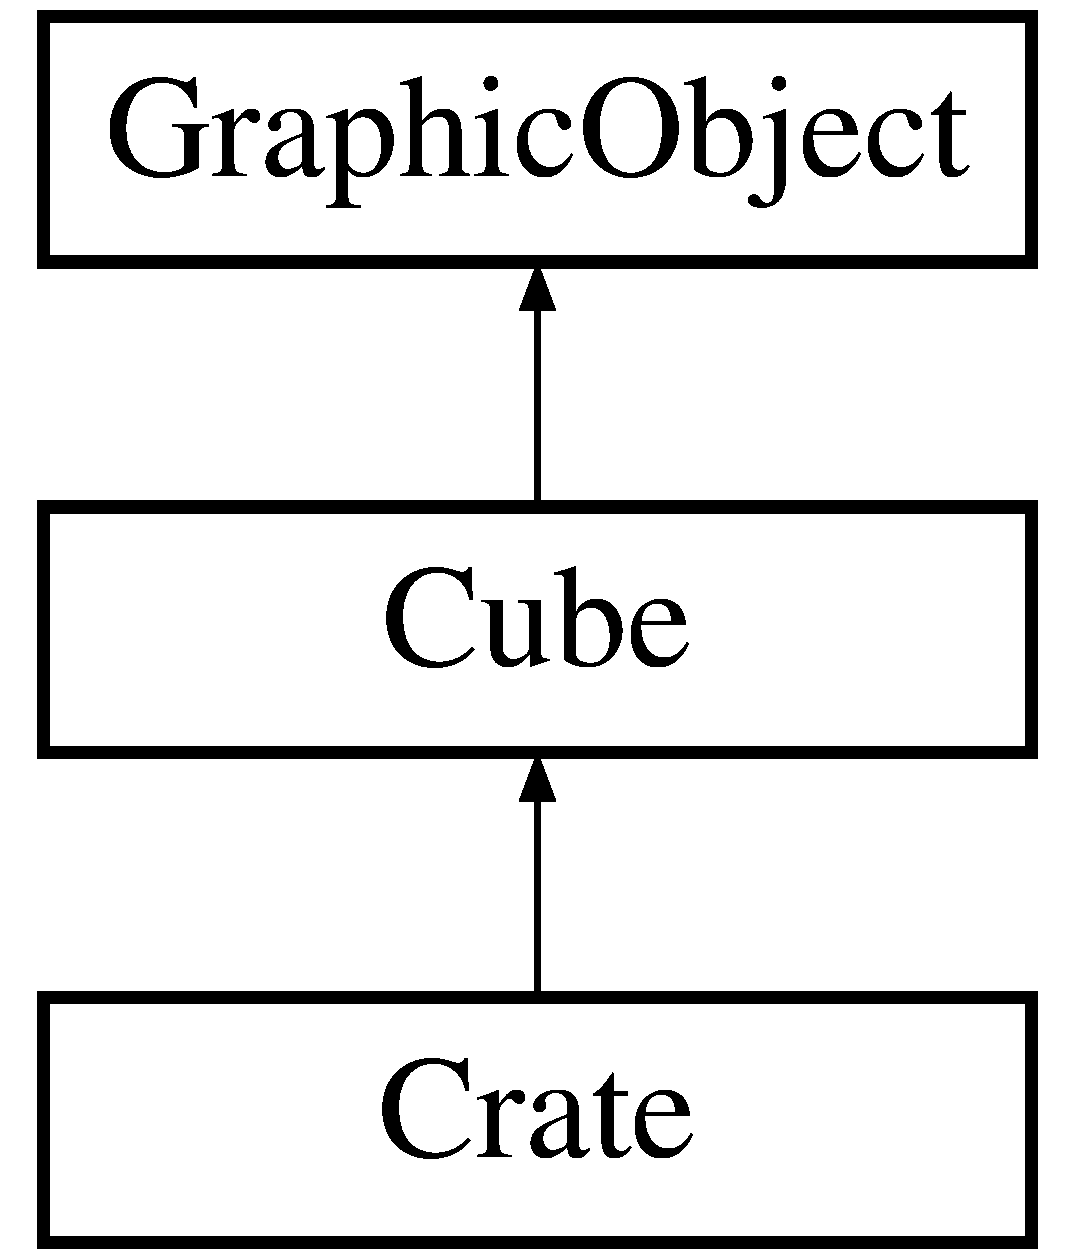
\includegraphics[height=3.000000cm]{classCrate}
\end{center}
\end{figure}
\subsection*{Public Member Functions}
\begin{DoxyCompactItemize}
\item 
\hypertarget{classCrate_ae8b4fbf45d678c405bfadb1d632ac98d}{}{\bfseries Crate} (float x, float y, float z, glm\+::vec4 dimensions, float size, std\+::string const \&vertex\+Shader, std\+::string const \&fragment\+Shader, std\+::string const \&texture)\label{classCrate_ae8b4fbf45d678c405bfadb1d632ac98d}

\item 
\hypertarget{classCrate_a0ea206abfee83e8114ae8bf3ab5acd59}{}{\bfseries Crate} (int x, int y, int z, glm\+::vec4 dimensions, float size, std\+::string const \&texture)\label{classCrate_a0ea206abfee83e8114ae8bf3ab5acd59}

\item 
void \hyperlink{classCrate_a0ef280ead61384d18817071ef85041d3}{draw} (glm\+::mat4 \&projection, glm\+::mat4 \&modelview)
\begin{DoxyCompactList}\small\item\em Displays the graphic object. \end{DoxyCompactList}\item 
\hypertarget{classCrate_a5a1c16623dae0656d9cc13260d1d227b}{}void \hyperlink{classCrate_a5a1c16623dae0656d9cc13260d1d227b}{load} ()\label{classCrate_a5a1c16623dae0656d9cc13260d1d227b}

\begin{DoxyCompactList}\small\item\em Creates the Open\+G\+L resources (V\+B\+O \& V\+A\+O) and sends the data to the graphic card. \end{DoxyCompactList}\item 
int \hyperlink{classCrate_a29df7675912f47eddd3a32010a8611fd}{nb\+Texture\+Bytes} ()
\begin{DoxyCompactList}\small\item\em Gives the memory size of the texture coordinates in bytes. \end{DoxyCompactList}\item 
\hypertarget{classCrate_aa52ebd20025131701e8b41986f318057}{}void {\bfseries print} ()\label{classCrate_aa52ebd20025131701e8b41986f318057}

\end{DoxyCompactItemize}
\subsection*{Protected Attributes}
\begin{DoxyCompactItemize}
\item 
std\+::shared\+\_\+ptr$<$ \hyperlink{classTexture}{Texture} $>$ \hyperlink{classCrate_aabfd1507281c170c5f21e40fa59db5d5}{texture\+\_\+}
\begin{DoxyCompactList}\small\item\em The texture manager. \end{DoxyCompactList}\item 
\hypertarget{classCrate_a05ac7fcd76d14fe4c21413ef041b4011}{}std\+::vector$<$ float $>$ \hyperlink{classCrate_a05ac7fcd76d14fe4c21413ef041b4011}{texture\+Coord\+\_\+}\label{classCrate_a05ac7fcd76d14fe4c21413ef041b4011}

\begin{DoxyCompactList}\small\item\em The texture coordinates stored in a 1\+D array for Open\+G\+L conviniency. \end{DoxyCompactList}\item 
\hypertarget{classCrate_a3235c603f229deb8091b53b19b70d0c0}{}glm\+::vec4 \hyperlink{classCrate_a3235c603f229deb8091b53b19b70d0c0}{dimensions\+\_\+}\label{classCrate_a3235c603f229deb8091b53b19b70d0c0}

\begin{DoxyCompactList}\small\item\em Other dimensions which will be managed in shaders. \end{DoxyCompactList}\end{DoxyCompactItemize}


\subsection{Detailed Description}
The \hyperlink{classCrate}{Crate} class. 

Textured cube. Uses the Flyweight pattern with a shared texture pool 

\subsection{Member Function Documentation}
\hypertarget{classCrate_a0ef280ead61384d18817071ef85041d3}{}\index{Crate@{Crate}!draw@{draw}}
\index{draw@{draw}!Crate@{Crate}}
\subsubsection[{draw}]{\setlength{\rightskip}{0pt plus 5cm}void Crate\+::draw (
\begin{DoxyParamCaption}
\item[{glm\+::mat4 \&}]{projection, }
\item[{glm\+::mat4 \&}]{modelview}
\end{DoxyParamCaption}
)\hspace{0.3cm}{\ttfamily [virtual]}}\label{classCrate_a0ef280ead61384d18817071ef85041d3}


Displays the graphic object. 


\begin{DoxyParams}{Parameters}
{\em projection} & The Open\+G\+L projection matrix \\
\hline
{\em modelview} & The Open\+G\+L modelview matrix, which is the product of the model matrix and the view matrix, in this order \\
\hline
\end{DoxyParams}


Implements \hyperlink{classGraphicObject_aacdc39f9e0b36ebb5c815e8bba717d7e}{Graphic\+Object}.

\hypertarget{classCrate_a29df7675912f47eddd3a32010a8611fd}{}\index{Crate@{Crate}!nb\+Texture\+Bytes@{nb\+Texture\+Bytes}}
\index{nb\+Texture\+Bytes@{nb\+Texture\+Bytes}!Crate@{Crate}}
\subsubsection[{nb\+Texture\+Bytes}]{\setlength{\rightskip}{0pt plus 5cm}int Crate\+::nb\+Texture\+Bytes (
\begin{DoxyParamCaption}
{}
\end{DoxyParamCaption}
)}\label{classCrate_a29df7675912f47eddd3a32010a8611fd}


Gives the memory size of the texture coordinates in bytes. 

\begin{DoxyReturn}{Returns}
The memory size of the texture coordinates in bytes 
\end{DoxyReturn}


\subsection{Member Data Documentation}
\hypertarget{classCrate_aabfd1507281c170c5f21e40fa59db5d5}{}\index{Crate@{Crate}!texture\+\_\+@{texture\+\_\+}}
\index{texture\+\_\+@{texture\+\_\+}!Crate@{Crate}}
\subsubsection[{texture\+\_\+}]{\setlength{\rightskip}{0pt plus 5cm}std\+::shared\+\_\+ptr$<${\bf Texture}$>$ Crate\+::texture\+\_\+\hspace{0.3cm}{\ttfamily [protected]}}\label{classCrate_aabfd1507281c170c5f21e40fa59db5d5}


The texture manager. 

A crate only has 1 texture which is repeated on all 6 faces 

The documentation for this class was generated from the following files\+:\begin{DoxyCompactItemize}
\item 
\hyperlink{Crate_8h}{Crate.\+h}\item 
Crate.\+cpp\end{DoxyCompactItemize}

\hypertarget{classCube}{}\section{Cube Class Reference}
\label{classCube}\index{Cube@{Cube}}


The \hyperlink{classCube}{Cube} class.  




{\ttfamily \#include $<$Cube.\+h$>$}

Inheritance diagram for Cube\+:\begin{figure}[H]
\begin{center}
\leavevmode
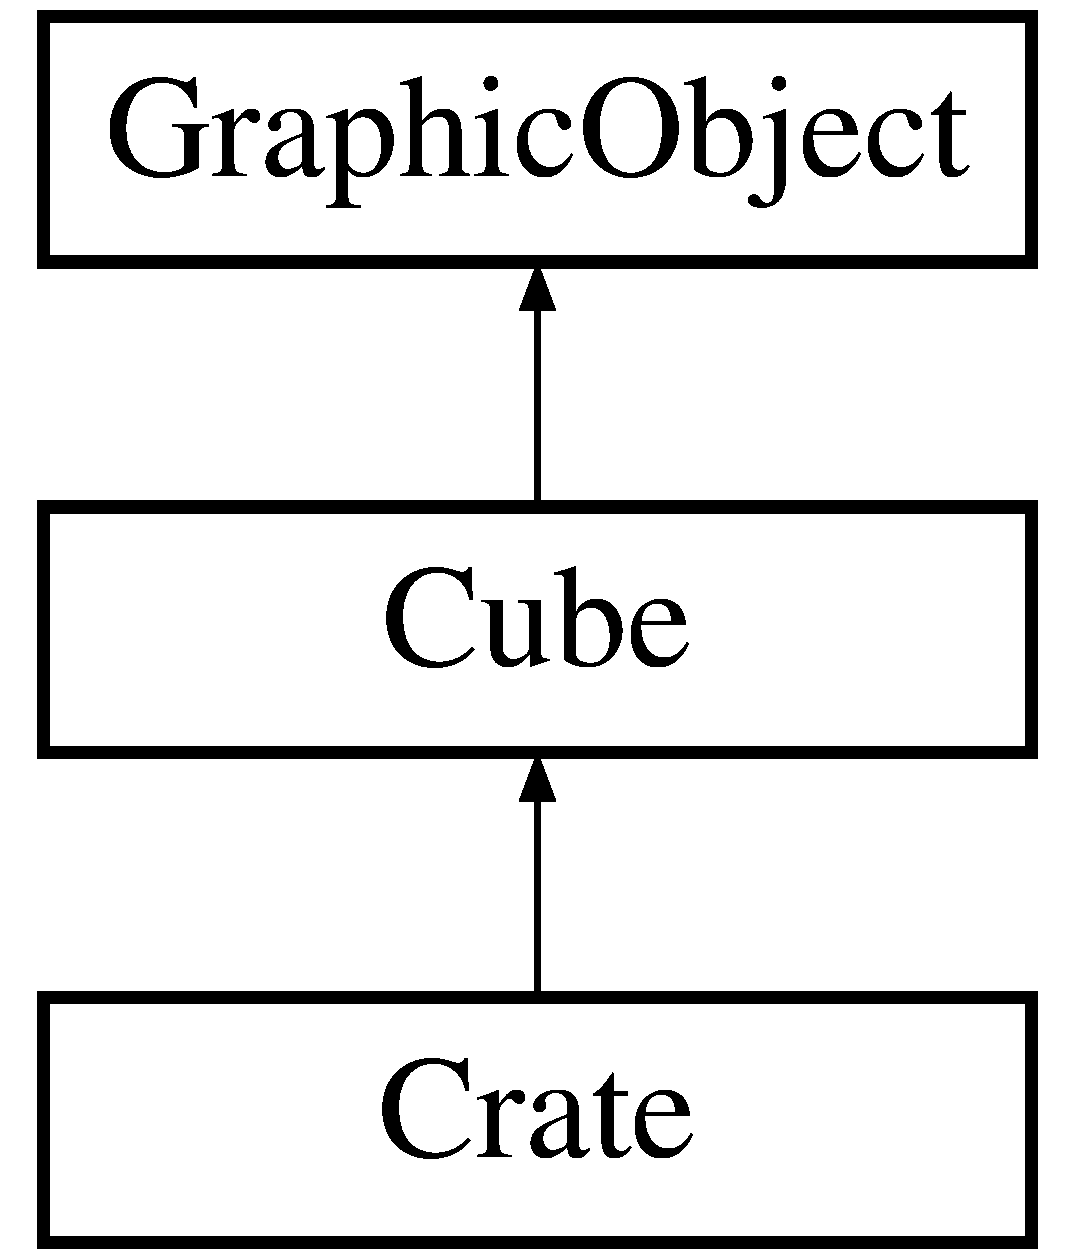
\includegraphics[height=3.000000cm]{classCube}
\end{center}
\end{figure}
\subsection*{Public Member Functions}
\begin{DoxyCompactItemize}
\item 
\hypertarget{classCube_ab8c70b8c650e3beaf14e4cbc21fec119}{}{\bfseries Cube} (float x, float y, float z, float size, std\+::string const \&vertex\+Shader, std\+::string const \&fragment\+Shader)\label{classCube_ab8c70b8c650e3beaf14e4cbc21fec119}

\item 
\hypertarget{classCube_a52ff32bc507c650318f23454388bfd61}{}{\bfseries Cube} (int x, int y, int z, float size)\label{classCube_a52ff32bc507c650318f23454388bfd61}

\item 
void \hyperlink{classCube_a4646f297e874e0dad42288ad153fc761}{draw} (glm\+::mat4 \&projection, glm\+::mat4 \&modelview)
\begin{DoxyCompactList}\small\item\em Displays the graphic object. \end{DoxyCompactList}\item 
\hypertarget{classCube_aa1326a13ad32a031f8c8f9bcf8f63b2a}{}virtual void \hyperlink{classCube_aa1326a13ad32a031f8c8f9bcf8f63b2a}{load} ()\label{classCube_aa1326a13ad32a031f8c8f9bcf8f63b2a}

\begin{DoxyCompactList}\small\item\em Creates the Open\+G\+L resources (V\+B\+O \& V\+A\+O) and sends the data to the graphic card. \end{DoxyCompactList}\end{DoxyCompactItemize}
\subsection*{Additional Inherited Members}


\subsection{Detailed Description}
The \hyperlink{classCube}{Cube} class. 

A non textured, colored \hyperlink{classCube}{Cube} 

\subsection{Member Function Documentation}
\hypertarget{classCube_a4646f297e874e0dad42288ad153fc761}{}\index{Cube@{Cube}!draw@{draw}}
\index{draw@{draw}!Cube@{Cube}}
\subsubsection[{draw}]{\setlength{\rightskip}{0pt plus 5cm}void Cube\+::draw (
\begin{DoxyParamCaption}
\item[{glm\+::mat4 \&}]{projection, }
\item[{glm\+::mat4 \&}]{modelview}
\end{DoxyParamCaption}
)\hspace{0.3cm}{\ttfamily [virtual]}}\label{classCube_a4646f297e874e0dad42288ad153fc761}


Displays the graphic object. 


\begin{DoxyParams}{Parameters}
{\em projection} & The Open\+G\+L projection matrix \\
\hline
{\em modelview} & The Open\+G\+L modelview matrix, which is the product of the model matrix and the view matrix, in this order \\
\hline
\end{DoxyParams}


Implements \hyperlink{classGraphicObject_aacdc39f9e0b36ebb5c815e8bba717d7e}{Graphic\+Object}.



The documentation for this class was generated from the following files\+:\begin{DoxyCompactItemize}
\item 
\hyperlink{Cube_8h}{Cube.\+h}\item 
Cube.\+cpp\end{DoxyCompactItemize}

\hypertarget{classFile}{}\section{File Class Reference}
\label{classFile}\index{File@{File}}
\subsection*{Public Member Functions}
\begin{DoxyCompactItemize}
\item 
\hyperlink{classFile_ae039af5807fc385f41b60644725d15d0}{File} ()
\begin{DoxyCompactList}\small\item\em \hyperlink{classFile_ae039af5807fc385f41b60644725d15d0}{File\+::\+File}. \end{DoxyCompactList}\item 
\hypertarget{classFile_abd2dacf27133c9d5595ecc414299f1a3}{}{\bfseries File} (std\+::string filename)\label{classFile_abd2dacf27133c9d5595ecc414299f1a3}

\item 
int \hyperlink{classFile_ad1024f9c4c3c48083f024aefaf45b9b8}{get\+Total\+Lines} ()
\begin{DoxyCompactList}\small\item\em \hyperlink{classFile_ad1024f9c4c3c48083f024aefaf45b9b8}{File\+::get\+Total\+Lines}. \end{DoxyCompactList}\item 
int \hyperlink{classFile_ab18dbfe80270e02ebb5e11754c30baa2}{get\+Total\+Lines\+Cah} ()
\begin{DoxyCompactList}\small\item\em \hyperlink{classFile_ab18dbfe80270e02ebb5e11754c30baa2}{File\+::get\+Total\+Lines\+Cah}. \end{DoxyCompactList}\item 
double \hyperlink{classFile_a3869cf9e61963974d68005449e47b0a5}{get\+Age} ()
\begin{DoxyCompactList}\small\item\em File\+::age\+\_\+. \end{DoxyCompactList}\item 
double \hyperlink{classFile_a9e40fb995d13f0ed06ef1d56508eb8ed}{get\+X\+Center\+Tp} ()
\begin{DoxyCompactList}\small\item\em File\+::x\+Center\+Tp\+\_\+. \end{DoxyCompactList}\item 
double \hyperlink{classFile_a1f9f5945b6d122bd4fbed4ea02596e8c}{get\+Y\+Center\+Tp} ()
\begin{DoxyCompactList}\small\item\em File\+::y\+Center\+Tp\+\_\+. \end{DoxyCompactList}\item 
double \hyperlink{classFile_a66dad0937bbef79d22bfca7428e9c5b8}{get\+Z\+Center\+Tp} ()
\begin{DoxyCompactList}\small\item\em File\+::y\+Center\+Tp\+\_\+. \end{DoxyCompactList}\item 
double \hyperlink{classFile_ab59ff015aacc745232543dfde488a98e}{get\+Size\+Scene} ()
\begin{DoxyCompactList}\small\item\em \hyperlink{classFile_ab59ff015aacc745232543dfde488a98e}{File\+::get\+Size\+Scene}. \end{DoxyCompactList}\item 
void \hyperlink{classFile_a4843f3a7a5bfaa86d11dbbf0adac7f0d}{set\+Size\+Scene} (int size\+Scene)
\begin{DoxyCompactList}\small\item\em \hyperlink{classFile_a4843f3a7a5bfaa86d11dbbf0adac7f0d}{File\+::set\+Size\+Scene}. \end{DoxyCompactList}\item 
\hypertarget{classFile_a6ff77386e6bb7c109ae83f2b00d1b75d}{}double {\bfseries get\+Max\+Tp} ()\label{classFile_a6ff77386e6bb7c109ae83f2b00d1b75d}

\item 
double $\ast$$\ast$ \hyperlink{classFile_a982f88fed4bf555b9f3ba69c37b5f0a7}{get\+Data} ()
\begin{DoxyCompactList}\small\item\em \hyperlink{classFile_a982f88fed4bf555b9f3ba69c37b5f0a7}{File\+::get\+Data}. \end{DoxyCompactList}\item 
double $\ast$$\ast$ \hyperlink{classFile_a8f59da39256bf141404043e3a93f9654}{get\+Data\+Cah} ()
\begin{DoxyCompactList}\small\item\em \hyperlink{classFile_a8f59da39256bf141404043e3a93f9654}{File\+::get\+Data\+Cah}. \end{DoxyCompactList}\item 
double \hyperlink{classFile_abf8e0e8e4e7d8a4ff99e327a8d30c394}{get\+Max\+Mass} ()
\begin{DoxyCompactList}\small\item\em \hyperlink{classFile_abf8e0e8e4e7d8a4ff99e327a8d30c394}{File\+::get\+Max\+Mass}. \end{DoxyCompactList}\item 
double \hyperlink{classFile_ab9f463bb8afd01c69d323872e2f3d275}{get\+Max\+Age} ()
\begin{DoxyCompactList}\small\item\em \hyperlink{classFile_ab9f463bb8afd01c69d323872e2f3d275}{File\+::get\+Max\+Age}. \end{DoxyCompactList}\item 
void \hyperlink{classFile_a986cac1668c92bf580eb20244fefab02}{parse\+Text} (bool compute\+Center\+Tp)
\begin{DoxyCompactList}\small\item\em \hyperlink{classFile_a986cac1668c92bf580eb20244fefab02}{File\+::parse\+Text}. \end{DoxyCompactList}\item 
void \hyperlink{classFile_a152b94a16617a9df570352696bfea31a}{exists\+\_\+test} ()
\begin{DoxyCompactList}\small\item\em \hyperlink{classFile_a152b94a16617a9df570352696bfea31a}{File\+::exists\+\_\+test}. \end{DoxyCompactList}\item 
int \hyperlink{classFile_acdb459909f2c43d3a4d84426276b41c3}{get\+Count} (std\+::string text, std\+::regex regex)
\begin{DoxyCompactList}\small\item\em \hyperlink{classFile_acdb459909f2c43d3a4d84426276b41c3}{File\+::get\+Count}. \end{DoxyCompactList}\item 
std\+::sregex\+\_\+iterator \hyperlink{classFile_ae8c20cf8ad1fdfcb7ac3532e1e8ed15f}{split} (std\+::string text, std\+::regex regex)
\begin{DoxyCompactList}\small\item\em \hyperlink{classFile_ae8c20cf8ad1fdfcb7ac3532e1e8ed15f}{File\+::split}. \end{DoxyCompactList}\item 
std\+::sregex\+\_\+iterator \hyperlink{classFile_a6a8d457f6b0ef7e8cf7d672381ad054a}{check\+If\+Exception\+In\+File} (std\+::string text, std\+::regex regex, int $\ast$i, bool compute\+Center\+Tp)
\begin{DoxyCompactList}\small\item\em \hyperlink{classFile_a6a8d457f6b0ef7e8cf7d672381ad054a}{File\+::check\+If\+Exception\+In\+File}. \end{DoxyCompactList}\item 
void \hyperlink{classFile_ac1dfd9873063fc9d40847e2df6a5f457}{register\+Data} (std\+::sregex\+\_\+iterator words\+\_\+begin, std\+::sregex\+\_\+iterator words\+\_\+end, int i, bool skip, bool compute\+Center\+Tp)
\begin{DoxyCompactList}\small\item\em \hyperlink{classFile_ac1dfd9873063fc9d40847e2df6a5f457}{File\+::register\+Data}. \end{DoxyCompactList}\item 
void \hyperlink{classFile_aa75c53588959985b64fa8e2f83ce1723}{update\+Max} (double new\+Age, int i)
\begin{DoxyCompactList}\small\item\em update\+Max \end{DoxyCompactList}\item 
void \hyperlink{classFile_a45db1a62b806343e520adb535ef6417a}{print\+Data} ()
\begin{DoxyCompactList}\small\item\em \hyperlink{classFile_a45db1a62b806343e520adb535ef6417a}{File\+::print\+Data}. \end{DoxyCompactList}\item 
int \hyperlink{classFile_a9af2773d1dd86d3e95e830563a51e3b5}{convert} (double d)
\begin{DoxyCompactList}\small\item\em \hyperlink{classFile_a9af2773d1dd86d3e95e830563a51e3b5}{File\+::convert}. \end{DoxyCompactList}\item 
\hypertarget{classFile_a9ba7a94c8022986138d194a02b9f3396}{}double {\bfseries convert\+To\+File} (double d)\label{classFile_a9ba7a94c8022986138d194a02b9f3396}

\item 
void \hyperlink{classFile_a4714786d79812c9aa720403af5a43210}{cah} (int cluster)
\begin{DoxyCompactList}\small\item\em \hyperlink{classFile_a4714786d79812c9aa720403af5a43210}{File\+::cah}. \end{DoxyCompactList}\item 
double \hyperlink{classFile_aba34124d22699d7cb26bcbeb85bef0f8}{dissim\+Max} (std\+::vector$<$ int $>$ c1, std\+::vector$<$ int $>$ c2)
\begin{DoxyCompactList}\small\item\em \hyperlink{classFile_aba34124d22699d7cb26bcbeb85bef0f8}{File\+::dissim\+Max}. \end{DoxyCompactList}\item 
double \hyperlink{classFile_a0db1da2014c0f1ac9253efe86c0a57d8}{dissim\+G} (std\+::vector$<$ int $>$ c1, std\+::vector$<$ int $>$ c2)
\begin{DoxyCompactList}\small\item\em \hyperlink{classFile_a0db1da2014c0f1ac9253efe86c0a57d8}{File\+::dissim\+G}. \end{DoxyCompactList}\item 
double \hyperlink{classFile_a42bd0e57ed74e6243e47a0f8ce187bb8}{dissim\+Alea} (std\+::vector$<$ int $>$ c1, std\+::vector$<$ int $>$ c2)
\begin{DoxyCompactList}\small\item\em \hyperlink{classFile_a42bd0e57ed74e6243e47a0f8ce187bb8}{File\+::dissim\+Alea}. \end{DoxyCompactList}\item 
std\+::vector$<$ int $>$ \hyperlink{classFile_a2fb2437e094b917b7d5d9836a75e5d4f}{min\+Mat\+Dissim} (double $\ast$$\ast$m, int size)
\begin{DoxyCompactList}\small\item\em \hyperlink{classFile_a2fb2437e094b917b7d5d9836a75e5d4f}{File\+::min\+Mat\+Dissim}. \end{DoxyCompactList}\item 
void \hyperlink{classFile_a311c46b95241183e414757bb52f79f7a}{register\+Clusters} ()
\begin{DoxyCompactList}\small\item\em File\+::register\+Cluster. \end{DoxyCompactList}\item 
void \hyperlink{classFile_afc54ef20547ada0b2bc0c1f7a0a939f1}{print\+Data\+Cah} ()
\begin{DoxyCompactList}\small\item\em \hyperlink{classFile_afc54ef20547ada0b2bc0c1f7a0a939f1}{File\+::print\+Data\+Cah}. \end{DoxyCompactList}\end{DoxyCompactItemize}
\subsection*{Public Attributes}
\begin{DoxyCompactItemize}
\item 
\hypertarget{classFile_adab8322f89fe09fe84a4943fe0fc1336}{}int {\bfseries mass} = 1\label{classFile_adab8322f89fe09fe84a4943fe0fc1336}

\item 
\hypertarget{classFile_a1bfba5df70c9b10c34f0716e94061e23}{}int {\bfseries xpos} = 2\label{classFile_a1bfba5df70c9b10c34f0716e94061e23}

\item 
\hypertarget{classFile_a84ecd2148a0141a2b1165ee8bca04df1}{}int {\bfseries ypos} = 3\label{classFile_a84ecd2148a0141a2b1165ee8bca04df1}

\item 
\hypertarget{classFile_a922087f19fc52541c93c7868fcf45a6f}{}int {\bfseries zpos} = 4\label{classFile_a922087f19fc52541c93c7868fcf45a6f}

\item 
\hypertarget{classFile_a6f0c6875caa36946f4c9c7453a47da1e}{}int {\bfseries age} = 5\label{classFile_a6f0c6875caa36946f4c9c7453a47da1e}

\item 
\hypertarget{classFile_a4de643e921715b3513cdd3f578eed54f}{}double {\bfseries Min\+Cube\+Size} = 0.\+3\label{classFile_a4de643e921715b3513cdd3f578eed54f}

\end{DoxyCompactItemize}


\subsection{Constructor \& Destructor Documentation}
\hypertarget{classFile_ae039af5807fc385f41b60644725d15d0}{}\index{File@{File}!File@{File}}
\index{File@{File}!File@{File}}
\subsubsection[{File}]{\setlength{\rightskip}{0pt plus 5cm}File\+::\+File (
\begin{DoxyParamCaption}
{}
\end{DoxyParamCaption}
)}\label{classFile_ae039af5807fc385f41b60644725d15d0}


\hyperlink{classFile_ae039af5807fc385f41b60644725d15d0}{File\+::\+File}. 

\hyperlink{classFile}{File} class Version 2.\+0. Put data in double$\ast$$\ast$ File\+::data\+\_\+. Use \hyperlink{classFile_a45db1a62b806343e520adb535ef6417a}{File\+::print\+Data()} to print them. Recognize n dimension. Uses the Regular Expression \char`\"{}(\mbox{[}$^\wedge$\textbackslash{}\textbackslash{}s\mbox{]}+)\char`\"{}. =$>$ Should be possible to read something like \+: \textquotesingle{}a b c d e\textquotesingle{}. Automatically detects the dimension (n) by reading the 3rd line. If a line is empty, it is ignored. If a line has not the same number of columns, it is ignored. 

\subsection{Member Function Documentation}
\hypertarget{classFile_a4714786d79812c9aa720403af5a43210}{}\index{File@{File}!cah@{cah}}
\index{cah@{cah}!File@{File}}
\subsubsection[{cah}]{\setlength{\rightskip}{0pt plus 5cm}void File\+::cah (
\begin{DoxyParamCaption}
\item[{int}]{cluster}
\end{DoxyParamCaption}
)}\label{classFile_a4714786d79812c9aa720403af5a43210}


\hyperlink{classFile_a4714786d79812c9aa720403af5a43210}{File\+::cah}. 

Compute a Hierarchical Clustering (C\+A\+H in french), clustering is saved into clusters\+\_\+ 
\begin{DoxyParams}{Parameters}
{\em cluster,the} & number of clusters \\
\hline
\end{DoxyParams}
\hypertarget{classFile_a6a8d457f6b0ef7e8cf7d672381ad054a}{}\index{File@{File}!check\+If\+Exception\+In\+File@{check\+If\+Exception\+In\+File}}
\index{check\+If\+Exception\+In\+File@{check\+If\+Exception\+In\+File}!File@{File}}
\subsubsection[{check\+If\+Exception\+In\+File}]{\setlength{\rightskip}{0pt plus 5cm}std\+::sregex\+\_\+iterator File\+::check\+If\+Exception\+In\+File (
\begin{DoxyParamCaption}
\item[{std\+::string}]{text, }
\item[{std\+::regex}]{regex, }
\item[{int $\ast$}]{i, }
\item[{bool}]{compute\+Center\+Tp}
\end{DoxyParamCaption}
)}\label{classFile_a6a8d457f6b0ef7e8cf7d672381ad054a}


\hyperlink{classFile_a6a8d457f6b0ef7e8cf7d672381ad054a}{File\+::check\+If\+Exception\+In\+File}. 

Check if there is an exception in the file. (1 line has more column). 
\begin{DoxyParams}{Parameters}
{\em text} & \\
\hline
{\em regex} & \\
\hline
{\em i} & \\
\hline
\end{DoxyParams}
\begin{DoxyReturn}{Returns}

\end{DoxyReturn}
\hypertarget{classFile_a9af2773d1dd86d3e95e830563a51e3b5}{}\index{File@{File}!convert@{convert}}
\index{convert@{convert}!File@{File}}
\subsubsection[{convert}]{\setlength{\rightskip}{0pt plus 5cm}int File\+::convert (
\begin{DoxyParamCaption}
\item[{double}]{d}
\end{DoxyParamCaption}
)}\label{classFile_a9af2773d1dd86d3e95e830563a51e3b5}


\hyperlink{classFile_a9af2773d1dd86d3e95e830563a51e3b5}{File\+::convert}. 

Convert coordonate from file to coordonate used in S\+D\+L. return data\mbox{[}i\mbox{]}\mbox{[}file\+\_\+.\+xpos\mbox{]}$\ast$(size\+Scene\+\_\+ -\/ 1) 
\begin{DoxyParams}{Parameters}
{\em d} & \\
\hline
\end{DoxyParams}
\hypertarget{classFile_a42bd0e57ed74e6243e47a0f8ce187bb8}{}\index{File@{File}!dissim\+Alea@{dissim\+Alea}}
\index{dissim\+Alea@{dissim\+Alea}!File@{File}}
\subsubsection[{dissim\+Alea}]{\setlength{\rightskip}{0pt plus 5cm}double File\+::dissim\+Alea (
\begin{DoxyParamCaption}
\item[{std\+::vector$<$ int $>$}]{c1, }
\item[{std\+::vector$<$ int $>$}]{c2}
\end{DoxyParamCaption}
)}\label{classFile_a42bd0e57ed74e6243e47a0f8ce187bb8}


\hyperlink{classFile_a42bd0e57ed74e6243e47a0f8ce187bb8}{File\+::dissim\+Alea}. 

Dissimetry between two clusters using distance between random points Doesn\textquotesingle{}t work 
\begin{DoxyParams}{Parameters}
{\em c1} & first cluster \\
\hline
{\em c2} & second cluster \\
\hline
\end{DoxyParams}
\hypertarget{classFile_a0db1da2014c0f1ac9253efe86c0a57d8}{}\index{File@{File}!dissim\+G@{dissim\+G}}
\index{dissim\+G@{dissim\+G}!File@{File}}
\subsubsection[{dissim\+G}]{\setlength{\rightskip}{0pt plus 5cm}double File\+::dissim\+G (
\begin{DoxyParamCaption}
\item[{std\+::vector$<$ int $>$}]{c1, }
\item[{std\+::vector$<$ int $>$}]{c2}
\end{DoxyParamCaption}
)}\label{classFile_a0db1da2014c0f1ac9253efe86c0a57d8}


\hyperlink{classFile_a0db1da2014c0f1ac9253efe86c0a57d8}{File\+::dissim\+G}. 

Dissimetry between two clusters using gravity center 
\begin{DoxyParams}{Parameters}
{\em c1} & first cluster \\
\hline
{\em c2} & second cluster \\
\hline
\end{DoxyParams}
\hypertarget{classFile_aba34124d22699d7cb26bcbeb85bef0f8}{}\index{File@{File}!dissim\+Max@{dissim\+Max}}
\index{dissim\+Max@{dissim\+Max}!File@{File}}
\subsubsection[{dissim\+Max}]{\setlength{\rightskip}{0pt plus 5cm}double File\+::dissim\+Max (
\begin{DoxyParamCaption}
\item[{std\+::vector$<$ int $>$}]{c1, }
\item[{std\+::vector$<$ int $>$}]{c2}
\end{DoxyParamCaption}
)}\label{classFile_aba34124d22699d7cb26bcbeb85bef0f8}


\hyperlink{classFile_aba34124d22699d7cb26bcbeb85bef0f8}{File\+::dissim\+Max}. 

Dissimetry between two clusters using maximum distance 
\begin{DoxyParams}{Parameters}
{\em c1} & first cluster \\
\hline
{\em c2} & second cluster \\
\hline
\end{DoxyParams}
\hypertarget{classFile_a152b94a16617a9df570352696bfea31a}{}\index{File@{File}!exists\+\_\+test@{exists\+\_\+test}}
\index{exists\+\_\+test@{exists\+\_\+test}!File@{File}}
\subsubsection[{exists\+\_\+test}]{\setlength{\rightskip}{0pt plus 5cm}void File\+::exists\+\_\+test (
\begin{DoxyParamCaption}
{}
\end{DoxyParamCaption}
)}\label{classFile_a152b94a16617a9df570352696bfea31a}


\hyperlink{classFile_a152b94a16617a9df570352696bfea31a}{File\+::exists\+\_\+test}. 

Test if the file filename\+\_\+ exists. \hypertarget{classFile_a3869cf9e61963974d68005449e47b0a5}{}\index{File@{File}!get\+Age@{get\+Age}}
\index{get\+Age@{get\+Age}!File@{File}}
\subsubsection[{get\+Age}]{\setlength{\rightskip}{0pt plus 5cm}double File\+::get\+Age (
\begin{DoxyParamCaption}
{}
\end{DoxyParamCaption}
)}\label{classFile_a3869cf9e61963974d68005449e47b0a5}


File\+::age\+\_\+. 

Getter of age\+\_\+ \hypertarget{classFile_acdb459909f2c43d3a4d84426276b41c3}{}\index{File@{File}!get\+Count@{get\+Count}}
\index{get\+Count@{get\+Count}!File@{File}}
\subsubsection[{get\+Count}]{\setlength{\rightskip}{0pt plus 5cm}int File\+::get\+Count (
\begin{DoxyParamCaption}
\item[{std\+::string}]{text, }
\item[{std\+::regex}]{regex}
\end{DoxyParamCaption}
)}\label{classFile_acdb459909f2c43d3a4d84426276b41c3}


\hyperlink{classFile_acdb459909f2c43d3a4d84426276b41c3}{File\+::get\+Count}. 

Count number of regex in a line. 
\begin{DoxyParams}{Parameters}
{\em text} & \\
\hline
{\em regex} & \\
\hline
\end{DoxyParams}
\begin{DoxyReturn}{Returns}

\end{DoxyReturn}
\hypertarget{classFile_a982f88fed4bf555b9f3ba69c37b5f0a7}{}\index{File@{File}!get\+Data@{get\+Data}}
\index{get\+Data@{get\+Data}!File@{File}}
\subsubsection[{get\+Data}]{\setlength{\rightskip}{0pt plus 5cm}double $\ast$$\ast$ File\+::get\+Data (
\begin{DoxyParamCaption}
{}
\end{DoxyParamCaption}
)}\label{classFile_a982f88fed4bf555b9f3ba69c37b5f0a7}


\hyperlink{classFile_a982f88fed4bf555b9f3ba69c37b5f0a7}{File\+::get\+Data}. 

Getter of data\+\_\+ \begin{DoxyReturn}{Returns}

\end{DoxyReturn}
\hypertarget{classFile_a8f59da39256bf141404043e3a93f9654}{}\index{File@{File}!get\+Data\+Cah@{get\+Data\+Cah}}
\index{get\+Data\+Cah@{get\+Data\+Cah}!File@{File}}
\subsubsection[{get\+Data\+Cah}]{\setlength{\rightskip}{0pt plus 5cm}double $\ast$$\ast$ File\+::get\+Data\+Cah (
\begin{DoxyParamCaption}
{}
\end{DoxyParamCaption}
)}\label{classFile_a8f59da39256bf141404043e3a93f9654}


\hyperlink{classFile_a8f59da39256bf141404043e3a93f9654}{File\+::get\+Data\+Cah}. 

Getter of data\+Cah\+\_\+ \begin{DoxyReturn}{Returns}

\end{DoxyReturn}
\hypertarget{classFile_ab9f463bb8afd01c69d323872e2f3d275}{}\index{File@{File}!get\+Max\+Age@{get\+Max\+Age}}
\index{get\+Max\+Age@{get\+Max\+Age}!File@{File}}
\subsubsection[{get\+Max\+Age}]{\setlength{\rightskip}{0pt plus 5cm}double File\+::get\+Max\+Age (
\begin{DoxyParamCaption}
{}
\end{DoxyParamCaption}
)}\label{classFile_ab9f463bb8afd01c69d323872e2f3d275}


\hyperlink{classFile_ab9f463bb8afd01c69d323872e2f3d275}{File\+::get\+Max\+Age}. 

Get the maximum of age data \hypertarget{classFile_abf8e0e8e4e7d8a4ff99e327a8d30c394}{}\index{File@{File}!get\+Max\+Mass@{get\+Max\+Mass}}
\index{get\+Max\+Mass@{get\+Max\+Mass}!File@{File}}
\subsubsection[{get\+Max\+Mass}]{\setlength{\rightskip}{0pt plus 5cm}double File\+::get\+Max\+Mass (
\begin{DoxyParamCaption}
{}
\end{DoxyParamCaption}
)}\label{classFile_abf8e0e8e4e7d8a4ff99e327a8d30c394}


\hyperlink{classFile_abf8e0e8e4e7d8a4ff99e327a8d30c394}{File\+::get\+Max\+Mass}. 

Get the maximum of mass data \hypertarget{classFile_ab59ff015aacc745232543dfde488a98e}{}\index{File@{File}!get\+Size\+Scene@{get\+Size\+Scene}}
\index{get\+Size\+Scene@{get\+Size\+Scene}!File@{File}}
\subsubsection[{get\+Size\+Scene}]{\setlength{\rightskip}{0pt plus 5cm}double File\+::get\+Size\+Scene (
\begin{DoxyParamCaption}
{}
\end{DoxyParamCaption}
)}\label{classFile_ab59ff015aacc745232543dfde488a98e}


\hyperlink{classFile_ab59ff015aacc745232543dfde488a98e}{File\+::get\+Size\+Scene}. 

Getter of size\+Scene\+\_\+ \begin{DoxyReturn}{Returns}

\end{DoxyReturn}
\hypertarget{classFile_ad1024f9c4c3c48083f024aefaf45b9b8}{}\index{File@{File}!get\+Total\+Lines@{get\+Total\+Lines}}
\index{get\+Total\+Lines@{get\+Total\+Lines}!File@{File}}
\subsubsection[{get\+Total\+Lines}]{\setlength{\rightskip}{0pt plus 5cm}int File\+::get\+Total\+Lines (
\begin{DoxyParamCaption}
{}
\end{DoxyParamCaption}
)}\label{classFile_ad1024f9c4c3c48083f024aefaf45b9b8}


\hyperlink{classFile_ad1024f9c4c3c48083f024aefaf45b9b8}{File\+::get\+Total\+Lines}. 

Getter of total\+Lines\+\_\+ \hypertarget{classFile_ab18dbfe80270e02ebb5e11754c30baa2}{}\index{File@{File}!get\+Total\+Lines\+Cah@{get\+Total\+Lines\+Cah}}
\index{get\+Total\+Lines\+Cah@{get\+Total\+Lines\+Cah}!File@{File}}
\subsubsection[{get\+Total\+Lines\+Cah}]{\setlength{\rightskip}{0pt plus 5cm}int File\+::get\+Total\+Lines\+Cah (
\begin{DoxyParamCaption}
{}
\end{DoxyParamCaption}
)}\label{classFile_ab18dbfe80270e02ebb5e11754c30baa2}


\hyperlink{classFile_ab18dbfe80270e02ebb5e11754c30baa2}{File\+::get\+Total\+Lines\+Cah}. 

Getter of total\+Lines\+Cah\+\_\+ \hypertarget{classFile_a9e40fb995d13f0ed06ef1d56508eb8ed}{}\index{File@{File}!get\+X\+Center\+Tp@{get\+X\+Center\+Tp}}
\index{get\+X\+Center\+Tp@{get\+X\+Center\+Tp}!File@{File}}
\subsubsection[{get\+X\+Center\+Tp}]{\setlength{\rightskip}{0pt plus 5cm}double File\+::get\+X\+Center\+Tp (
\begin{DoxyParamCaption}
{}
\end{DoxyParamCaption}
)}\label{classFile_a9e40fb995d13f0ed06ef1d56508eb8ed}


File\+::x\+Center\+Tp\+\_\+. 

Getter of x\+Center\+Tp\+\_\+ \hypertarget{classFile_a1f9f5945b6d122bd4fbed4ea02596e8c}{}\index{File@{File}!get\+Y\+Center\+Tp@{get\+Y\+Center\+Tp}}
\index{get\+Y\+Center\+Tp@{get\+Y\+Center\+Tp}!File@{File}}
\subsubsection[{get\+Y\+Center\+Tp}]{\setlength{\rightskip}{0pt plus 5cm}double File\+::get\+Y\+Center\+Tp (
\begin{DoxyParamCaption}
{}
\end{DoxyParamCaption}
)}\label{classFile_a1f9f5945b6d122bd4fbed4ea02596e8c}


File\+::y\+Center\+Tp\+\_\+. 

Getter of y\+Center\+Tp\+\_\+ \hypertarget{classFile_a66dad0937bbef79d22bfca7428e9c5b8}{}\index{File@{File}!get\+Z\+Center\+Tp@{get\+Z\+Center\+Tp}}
\index{get\+Z\+Center\+Tp@{get\+Z\+Center\+Tp}!File@{File}}
\subsubsection[{get\+Z\+Center\+Tp}]{\setlength{\rightskip}{0pt plus 5cm}double File\+::get\+Z\+Center\+Tp (
\begin{DoxyParamCaption}
{}
\end{DoxyParamCaption}
)}\label{classFile_a66dad0937bbef79d22bfca7428e9c5b8}


File\+::y\+Center\+Tp\+\_\+. 

Getter of y\+Center\+Tp\+\_\+ \hypertarget{classFile_a2fb2437e094b917b7d5d9836a75e5d4f}{}\index{File@{File}!min\+Mat\+Dissim@{min\+Mat\+Dissim}}
\index{min\+Mat\+Dissim@{min\+Mat\+Dissim}!File@{File}}
\subsubsection[{min\+Mat\+Dissim}]{\setlength{\rightskip}{0pt plus 5cm}std\+::vector$<$ int $>$ File\+::min\+Mat\+Dissim (
\begin{DoxyParamCaption}
\item[{double $\ast$$\ast$}]{m, }
\item[{int}]{size}
\end{DoxyParamCaption}
)}\label{classFile_a2fb2437e094b917b7d5d9836a75e5d4f}


\hyperlink{classFile_a2fb2437e094b917b7d5d9836a75e5d4f}{File\+::min\+Mat\+Dissim}. 

Minimum of a symetric square matrix 
\begin{DoxyParams}{Parameters}
{\em matrix} & m \\
\hline
{\em size} & of square matrix \\
\hline
\end{DoxyParams}
\hypertarget{classFile_a986cac1668c92bf580eb20244fefab02}{}\index{File@{File}!parse\+Text@{parse\+Text}}
\index{parse\+Text@{parse\+Text}!File@{File}}
\subsubsection[{parse\+Text}]{\setlength{\rightskip}{0pt plus 5cm}void File\+::parse\+Text (
\begin{DoxyParamCaption}
\item[{bool}]{compute\+Center\+Tp}
\end{DoxyParamCaption}
)}\label{classFile_a986cac1668c92bf580eb20244fefab02}


\hyperlink{classFile_a986cac1668c92bf580eb20244fefab02}{File\+::parse\+Text}. 

Parse text files using regex. Skip if line dimension is 0 (only blank). Stores data in\+\_\+data. 
\begin{DoxyParams}{Parameters}
{\em compute\+Center\+Tp} & yes to compute center of data. Use T to teleport to this center. \\
\hline
\end{DoxyParams}
\hypertarget{classFile_a45db1a62b806343e520adb535ef6417a}{}\index{File@{File}!print\+Data@{print\+Data}}
\index{print\+Data@{print\+Data}!File@{File}}
\subsubsection[{print\+Data}]{\setlength{\rightskip}{0pt plus 5cm}void File\+::print\+Data (
\begin{DoxyParamCaption}
{}
\end{DoxyParamCaption}
)}\label{classFile_a45db1a62b806343e520adb535ef6417a}


\hyperlink{classFile_a45db1a62b806343e520adb535ef6417a}{File\+::print\+Data}. 

Print all data stored in data\+\_\+. \hypertarget{classFile_afc54ef20547ada0b2bc0c1f7a0a939f1}{}\index{File@{File}!print\+Data\+Cah@{print\+Data\+Cah}}
\index{print\+Data\+Cah@{print\+Data\+Cah}!File@{File}}
\subsubsection[{print\+Data\+Cah}]{\setlength{\rightskip}{0pt plus 5cm}void File\+::print\+Data\+Cah (
\begin{DoxyParamCaption}
{}
\end{DoxyParamCaption}
)}\label{classFile_afc54ef20547ada0b2bc0c1f7a0a939f1}


\hyperlink{classFile_afc54ef20547ada0b2bc0c1f7a0a939f1}{File\+::print\+Data\+Cah}. 

Print all data stored in data\+Cah\+\_\+. \hypertarget{classFile_a311c46b95241183e414757bb52f79f7a}{}\index{File@{File}!register\+Clusters@{register\+Clusters}}
\index{register\+Clusters@{register\+Clusters}!File@{File}}
\subsubsection[{register\+Clusters}]{\setlength{\rightskip}{0pt plus 5cm}void File\+::register\+Clusters (
\begin{DoxyParamCaption}
{}
\end{DoxyParamCaption}
)}\label{classFile_a311c46b95241183e414757bb52f79f7a}


File\+::register\+Cluster. 

Register clusters to the array data\+Cah\+\_\+ 
\begin{DoxyParams}{Parameters}
{\em clusters} & \\
\hline
\end{DoxyParams}
\hypertarget{classFile_ac1dfd9873063fc9d40847e2df6a5f457}{}\index{File@{File}!register\+Data@{register\+Data}}
\index{register\+Data@{register\+Data}!File@{File}}
\subsubsection[{register\+Data}]{\setlength{\rightskip}{0pt plus 5cm}void File\+::register\+Data (
\begin{DoxyParamCaption}
\item[{std\+::sregex\+\_\+iterator}]{words\+\_\+begin, }
\item[{std\+::sregex\+\_\+iterator}]{words\+\_\+end, }
\item[{int}]{i, }
\item[{bool}]{skip, }
\item[{bool}]{compute\+Center\+Tp}
\end{DoxyParamCaption}
)}\label{classFile_ac1dfd9873063fc9d40847e2df6a5f457}


\hyperlink{classFile_ac1dfd9873063fc9d40847e2df6a5f457}{File\+::register\+Data}. 

Register data to the array, only launched if the line is valid. 
\begin{DoxyParams}{Parameters}
{\em words\+\_\+begin} & \\
\hline
{\em words\+\_\+end} & \\
\hline
{\em i} & \\
\hline
\end{DoxyParams}
\hypertarget{classFile_a4843f3a7a5bfaa86d11dbbf0adac7f0d}{}\index{File@{File}!set\+Size\+Scene@{set\+Size\+Scene}}
\index{set\+Size\+Scene@{set\+Size\+Scene}!File@{File}}
\subsubsection[{set\+Size\+Scene}]{\setlength{\rightskip}{0pt plus 5cm}void File\+::set\+Size\+Scene (
\begin{DoxyParamCaption}
\item[{int}]{size\+Scene}
\end{DoxyParamCaption}
)}\label{classFile_a4843f3a7a5bfaa86d11dbbf0adac7f0d}


\hyperlink{classFile_a4843f3a7a5bfaa86d11dbbf0adac7f0d}{File\+::set\+Size\+Scene}. 

Setter of size\+Scene\+\_\+ 
\begin{DoxyParams}{Parameters}
{\em size\+Scene} & \\
\hline
\end{DoxyParams}
\hypertarget{classFile_ae8c20cf8ad1fdfcb7ac3532e1e8ed15f}{}\index{File@{File}!split@{split}}
\index{split@{split}!File@{File}}
\subsubsection[{split}]{\setlength{\rightskip}{0pt plus 5cm}std\+::sregex\+\_\+iterator File\+::split (
\begin{DoxyParamCaption}
\item[{std\+::string}]{text, }
\item[{std\+::regex}]{regex}
\end{DoxyParamCaption}
)}\label{classFile_ae8c20cf8ad1fdfcb7ac3532e1e8ed15f}


\hyperlink{classFile_ae8c20cf8ad1fdfcb7ac3532e1e8ed15f}{File\+::split}. 

Split a text to an iterator with a regex. Use \hyperlink{classFile_ac1dfd9873063fc9d40847e2df6a5f457}{register\+Data()} to go throw the iterator. 
\begin{DoxyParams}{Parameters}
{\em text} & \\
\hline
{\em regex} & \\
\hline
\end{DoxyParams}
\begin{DoxyReturn}{Returns}

\end{DoxyReturn}
\hypertarget{classFile_aa75c53588959985b64fa8e2f83ce1723}{}\index{File@{File}!update\+Max@{update\+Max}}
\index{update\+Max@{update\+Max}!File@{File}}
\subsubsection[{update\+Max}]{\setlength{\rightskip}{0pt plus 5cm}void File\+::update\+Max (
\begin{DoxyParamCaption}
\item[{double}]{new\+Age, }
\item[{int}]{i}
\end{DoxyParamCaption}
)}\label{classFile_aa75c53588959985b64fa8e2f83ce1723}


update\+Max 

update max\+Tp\+\_\+ if age is smaller. 
\begin{DoxyParams}{Parameters}
{\em a} & \\
\hline
{\em b} & \\
\hline
\end{DoxyParams}
\begin{DoxyReturn}{Returns}

\end{DoxyReturn}


The documentation for this class was generated from the following files\+:\begin{DoxyCompactItemize}
\item 
File.\+h\item 
File.\+cpp\end{DoxyCompactItemize}

\hypertarget{classGenericOculus}{}\section{Generic\+Oculus Class Reference}
\label{classGenericOculus}\index{Generic\+Oculus@{Generic\+Oculus}}


The \hyperlink{classGenericOculus}{Generic\+Oculus} class.  




{\ttfamily \#include $<$Oculus.\+h$>$}

Inheritance diagram for Generic\+Oculus\+:\begin{figure}[H]
\begin{center}
\leavevmode
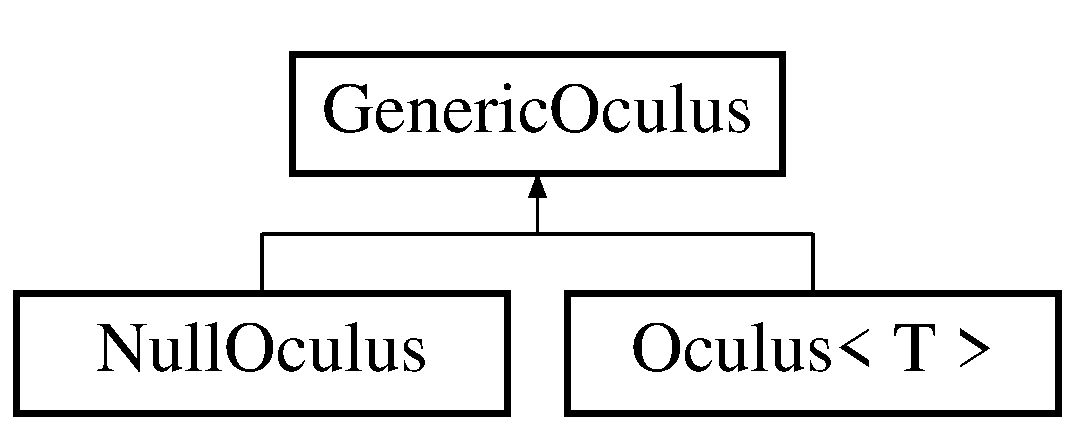
\includegraphics[height=2.000000cm]{classGenericOculus}
\end{center}
\end{figure}
\subsection*{Public Member Functions}
\begin{DoxyCompactItemize}
\item 
\hypertarget{classGenericOculus_a86a6f7f822d15f45ac6df6842b1dc4ce}{}virtual void {\bfseries render} ()=0\label{classGenericOculus_a86a6f7f822d15f45ac6df6842b1dc4ce}

\item 
\hypertarget{classGenericOculus_a80b6766dd4a710d6b75a2dc2e746b753}{}virtual void {\bfseries get\+Input} ()\label{classGenericOculus_a80b6766dd4a710d6b75a2dc2e746b753}

\item 
\hypertarget{classGenericOculus_a074b05f3be2cb859b00c49e779685276}{}virtual bool {\bfseries is\+Moving} () const \label{classGenericOculus_a074b05f3be2cb859b00c49e779685276}

\item 
\hypertarget{classGenericOculus_a5d62cc682f918c2cfad7d139b1ff3299}{}virtual bool {\bfseries is\+Using\+Debug\+Hmd} ()\label{classGenericOculus_a5d62cc682f918c2cfad7d139b1ff3299}

\item 
\hypertarget{classGenericOculus_ad679f6563497fa5b79f32d2295a32e6e}{}virtual glm\+::vec3 {\bfseries d\+Angles} () const \label{classGenericOculus_ad679f6563497fa5b79f32d2295a32e6e}

\end{DoxyCompactItemize}


\subsection{Detailed Description}
The \hyperlink{classGenericOculus}{Generic\+Oculus} class. 

The documentation for this class was generated from the following files\+:\begin{DoxyCompactItemize}
\item 
\hyperlink{Oculus_8h}{Oculus.\+h}\item 
Oculus.\+cpp\end{DoxyCompactItemize}

\hypertarget{classGraphicObject}{}\section{Graphic\+Object Class Reference}
\label{classGraphicObject}\index{Graphic\+Object@{Graphic\+Object}}


The \hyperlink{classGraphicObject}{Graphic\+Object} class.  




{\ttfamily \#include $<$Graphic\+Object.\+h$>$}

Inheritance diagram for Graphic\+Object\+:\begin{figure}[H]
\begin{center}
\leavevmode
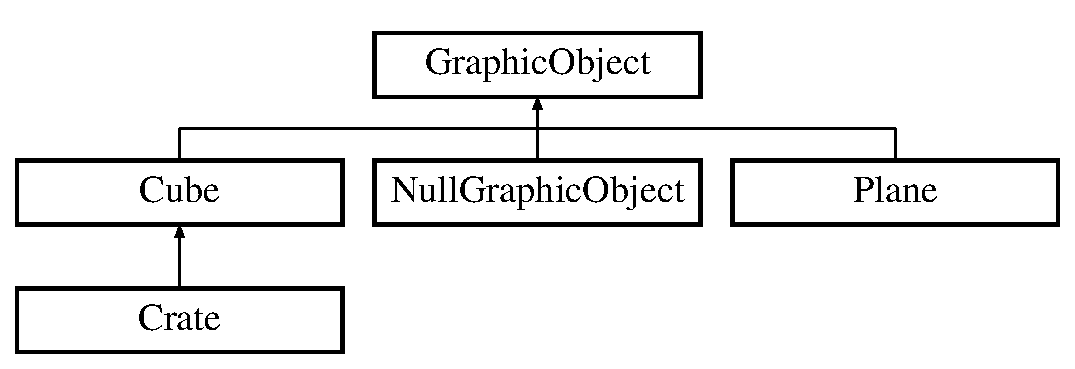
\includegraphics[height=3.000000cm]{classGraphicObject}
\end{center}
\end{figure}
\subsection*{Public Member Functions}
\begin{DoxyCompactItemize}
\item 
\hypertarget{classGraphicObject_a71f73b9dbb85a3a27d98aae1922120f4}{}{\bfseries Graphic\+Object} (float x=0, float y=0, float z=0, float size=0, std\+::string const \&vertex\+Shader=\char`\"{}\char`\"{}, std\+::string const \&fragment\+Shader=\char`\"{}\char`\"{})\label{classGraphicObject_a71f73b9dbb85a3a27d98aae1922120f4}

\item 
virtual void \hyperlink{classGraphicObject_aacdc39f9e0b36ebb5c815e8bba717d7e}{draw} (glm\+::mat4 \&projection, glm\+::mat4 \&modelview)=0
\begin{DoxyCompactList}\small\item\em Displays the graphic object. \end{DoxyCompactList}\item 
int \hyperlink{classGraphicObject_a8e43dbd70ae6a48bc53cf1b509791af0}{nb\+Vertices\+Bytes} ()
\begin{DoxyCompactList}\small\item\em Gives the memory size of the vertices coordinates in bytes. \end{DoxyCompactList}\item 
int \hyperlink{classGraphicObject_a9f4d774f94d51ebf0c44829898dbe012}{nb\+Colors\+Bytes} ()
\begin{DoxyCompactList}\small\item\em Gives the memory size of the colors coordinates in bytes. \end{DoxyCompactList}\item 
void \hyperlink{classGraphicObject_a797f54b07ba4ee40b496a011245d9d8c}{move} (glm\+::vec3 const \&value)
\begin{DoxyCompactList}\small\item\em Moves the object a given vector. \end{DoxyCompactList}\item 
\hypertarget{classGraphicObject_ab4fe774c59ee6d67547094f2410b7266}{}void {\bfseries update\+V\+B\+O} (void $\ast$data, int bytes\+Size, int offset)\label{classGraphicObject_ab4fe774c59ee6d67547094f2410b7266}

\end{DoxyCompactItemize}
\subsection*{Protected Attributes}
\begin{DoxyCompactItemize}
\item 
\hypertarget{classGraphicObject_a5bed301cfd29cea7e56e6e4b47c85c39}{}glm\+::vec3 \hyperlink{classGraphicObject_a5bed301cfd29cea7e56e6e4b47c85c39}{position\+\_\+}\label{classGraphicObject_a5bed301cfd29cea7e56e6e4b47c85c39}

\begin{DoxyCompactList}\small\item\em The position of the object. \end{DoxyCompactList}\item 
glm\+::vec3 \hyperlink{classGraphicObject_ad147f3d14ee99610b7ff2f6d50f601c9}{orientation\+\_\+}
\begin{DoxyCompactList}\small\item\em The orientation of the object. \end{DoxyCompactList}\item 
float \hyperlink{classGraphicObject_aaf5a021607b05779bd670fa912950bd1}{size\+\_\+}
\begin{DoxyCompactList}\small\item\em The size of the object. \end{DoxyCompactList}\item 
std\+::vector$<$ float $>$ \hyperlink{classGraphicObject_a911bfc9f48b22d0dbb3de68ff8a52ecf}{vertices\+\_\+}
\begin{DoxyCompactList}\small\item\em The vertices coordinates of the object. \end{DoxyCompactList}\item 
std\+::vector$<$ float $>$ \hyperlink{classGraphicObject_a58d16316152c9b216b0c258395f4ccb1}{colors\+\_\+}
\begin{DoxyCompactList}\small\item\em The colors coordinates of the object. \end{DoxyCompactList}\item 
std\+::unique\+\_\+ptr$<$ \hyperlink{classShader}{Shader} $>$ \hyperlink{classGraphicObject_a8ad07f4e11a71b5ed0d4fc66f14ab83e}{shader\+\_\+}
\begin{DoxyCompactList}\small\item\em The shader manager. \end{DoxyCompactList}\item 
\hypertarget{classGraphicObject_a8a25934d9b5af9b66ae731458a916db3}{}G\+Luint \hyperlink{classGraphicObject_a8a25934d9b5af9b66ae731458a916db3}{V\+B\+O\+Id\+\_\+}\label{classGraphicObject_a8a25934d9b5af9b66ae731458a916db3}

\begin{DoxyCompactList}\small\item\em The Open\+G\+L id of the Vertex Buffer Object which stores the vertices coordinates in the graphic card. \end{DoxyCompactList}\item 
\hypertarget{classGraphicObject_ad3c92aa937932b6effd095a2ce6ba6e9}{}G\+Luint \hyperlink{classGraphicObject_ad3c92aa937932b6effd095a2ce6ba6e9}{V\+A\+O\+Id\+\_\+}\label{classGraphicObject_ad3c92aa937932b6effd095a2ce6ba6e9}

\begin{DoxyCompactList}\small\item\em The Open\+G\+L id of the Vertex Array Object which stores multiple V\+B\+Os in the graphic card. \end{DoxyCompactList}\end{DoxyCompactItemize}


\subsection{Detailed Description}
The \hyperlink{classGraphicObject}{Graphic\+Object} class. 

Abstract base class for all graphic objects in the scene. 

\subsection{Member Function Documentation}
\hypertarget{classGraphicObject_aacdc39f9e0b36ebb5c815e8bba717d7e}{}\index{Graphic\+Object@{Graphic\+Object}!draw@{draw}}
\index{draw@{draw}!Graphic\+Object@{Graphic\+Object}}
\subsubsection[{draw}]{\setlength{\rightskip}{0pt plus 5cm}virtual void Graphic\+Object\+::draw (
\begin{DoxyParamCaption}
\item[{glm\+::mat4 \&}]{projection, }
\item[{glm\+::mat4 \&}]{modelview}
\end{DoxyParamCaption}
)\hspace{0.3cm}{\ttfamily [pure virtual]}}\label{classGraphicObject_aacdc39f9e0b36ebb5c815e8bba717d7e}


Displays the graphic object. 


\begin{DoxyParams}{Parameters}
{\em projection} & The Open\+G\+L projection matrix \\
\hline
{\em modelview} & The Open\+G\+L modelview matrix, which is the product of the model matrix and the view matrix, in this order \\
\hline
\end{DoxyParams}


Implemented in \hyperlink{classNullGraphicObject_a33c23cd19bac667ad7b1ccbcd9a373d2}{Null\+Graphic\+Object}, \hyperlink{classCrate_a0ef280ead61384d18817071ef85041d3}{Crate}, \hyperlink{classPlane_ac046dce6b4226e86fbcaf850fa7e30fd}{Plane}, and \hyperlink{classCube_a4646f297e874e0dad42288ad153fc761}{Cube}.

\hypertarget{classGraphicObject_a797f54b07ba4ee40b496a011245d9d8c}{}\index{Graphic\+Object@{Graphic\+Object}!move@{move}}
\index{move@{move}!Graphic\+Object@{Graphic\+Object}}
\subsubsection[{move}]{\setlength{\rightskip}{0pt plus 5cm}void Graphic\+Object\+::move (
\begin{DoxyParamCaption}
\item[{glm\+::vec3 const \&}]{value}
\end{DoxyParamCaption}
)}\label{classGraphicObject_a797f54b07ba4ee40b496a011245d9d8c}


Moves the object a given vector. 


\begin{DoxyParams}{Parameters}
{\em value} & The vector to add to the object position \\
\hline
\end{DoxyParams}
\hypertarget{classGraphicObject_a9f4d774f94d51ebf0c44829898dbe012}{}\index{Graphic\+Object@{Graphic\+Object}!nb\+Colors\+Bytes@{nb\+Colors\+Bytes}}
\index{nb\+Colors\+Bytes@{nb\+Colors\+Bytes}!Graphic\+Object@{Graphic\+Object}}
\subsubsection[{nb\+Colors\+Bytes}]{\setlength{\rightskip}{0pt plus 5cm}int Graphic\+Object\+::nb\+Colors\+Bytes (
\begin{DoxyParamCaption}
{}
\end{DoxyParamCaption}
)}\label{classGraphicObject_a9f4d774f94d51ebf0c44829898dbe012}


Gives the memory size of the colors coordinates in bytes. 

It is used to send the colors coordinates to the graphic card with a Vertex Buffer Object, indicating to Open\+G\+L how much memory this buffer takes \begin{DoxyReturn}{Returns}
The memory size of the colors coordinates in bytes 
\end{DoxyReturn}
\hypertarget{classGraphicObject_a8e43dbd70ae6a48bc53cf1b509791af0}{}\index{Graphic\+Object@{Graphic\+Object}!nb\+Vertices\+Bytes@{nb\+Vertices\+Bytes}}
\index{nb\+Vertices\+Bytes@{nb\+Vertices\+Bytes}!Graphic\+Object@{Graphic\+Object}}
\subsubsection[{nb\+Vertices\+Bytes}]{\setlength{\rightskip}{0pt plus 5cm}int Graphic\+Object\+::nb\+Vertices\+Bytes (
\begin{DoxyParamCaption}
{}
\end{DoxyParamCaption}
)}\label{classGraphicObject_a8e43dbd70ae6a48bc53cf1b509791af0}


Gives the memory size of the vertices coordinates in bytes. 

It is used to send the vertices coordinates to the graphic card with a Vertex Buffer Object, indicating to Open\+G\+L how much memory this buffer takes \begin{DoxyReturn}{Returns}
The memory size of the vertices coordinates in bytes 
\end{DoxyReturn}


\subsection{Member Data Documentation}
\hypertarget{classGraphicObject_a58d16316152c9b216b0c258395f4ccb1}{}\index{Graphic\+Object@{Graphic\+Object}!colors\+\_\+@{colors\+\_\+}}
\index{colors\+\_\+@{colors\+\_\+}!Graphic\+Object@{Graphic\+Object}}
\subsubsection[{colors\+\_\+}]{\setlength{\rightskip}{0pt plus 5cm}std\+::vector$<$float$>$ Graphic\+Object\+::colors\+\_\+\hspace{0.3cm}{\ttfamily [protected]}}\label{classGraphicObject_a58d16316152c9b216b0c258395f4ccb1}


The colors coordinates of the object. 

Open\+G\+L requires that these are given in a 1\+D array, so they are stored this way. These are ignored if the object is textured. \hypertarget{classGraphicObject_ad147f3d14ee99610b7ff2f6d50f601c9}{}\index{Graphic\+Object@{Graphic\+Object}!orientation\+\_\+@{orientation\+\_\+}}
\index{orientation\+\_\+@{orientation\+\_\+}!Graphic\+Object@{Graphic\+Object}}
\subsubsection[{orientation\+\_\+}]{\setlength{\rightskip}{0pt plus 5cm}glm\+::vec3 Graphic\+Object\+::orientation\+\_\+\hspace{0.3cm}{\ttfamily [protected]}}\label{classGraphicObject_ad147f3d14ee99610b7ff2f6d50f601c9}


The orientation of the object. 

Not used as of yet \hypertarget{classGraphicObject_a8ad07f4e11a71b5ed0d4fc66f14ab83e}{}\index{Graphic\+Object@{Graphic\+Object}!shader\+\_\+@{shader\+\_\+}}
\index{shader\+\_\+@{shader\+\_\+}!Graphic\+Object@{Graphic\+Object}}
\subsubsection[{shader\+\_\+}]{\setlength{\rightskip}{0pt plus 5cm}std\+::unique\+\_\+ptr$<${\bf Shader}$>$ Graphic\+Object\+::shader\+\_\+\hspace{0.3cm}{\ttfamily [protected]}}\label{classGraphicObject_a8ad07f4e11a71b5ed0d4fc66f14ab83e}


The shader manager. 

In Open\+G\+L $>$ 3.\+0 every object is displayed and tranformed through a shader. \hypertarget{classGraphicObject_aaf5a021607b05779bd670fa912950bd1}{}\index{Graphic\+Object@{Graphic\+Object}!size\+\_\+@{size\+\_\+}}
\index{size\+\_\+@{size\+\_\+}!Graphic\+Object@{Graphic\+Object}}
\subsubsection[{size\+\_\+}]{\setlength{\rightskip}{0pt plus 5cm}float Graphic\+Object\+::size\+\_\+\hspace{0.3cm}{\ttfamily [protected]}}\label{classGraphicObject_aaf5a021607b05779bd670fa912950bd1}


The size of the object. 

It is used to scale the object. By default its value is 1. \hypertarget{classGraphicObject_a911bfc9f48b22d0dbb3de68ff8a52ecf}{}\index{Graphic\+Object@{Graphic\+Object}!vertices\+\_\+@{vertices\+\_\+}}
\index{vertices\+\_\+@{vertices\+\_\+}!Graphic\+Object@{Graphic\+Object}}
\subsubsection[{vertices\+\_\+}]{\setlength{\rightskip}{0pt plus 5cm}std\+::vector$<$float$>$ Graphic\+Object\+::vertices\+\_\+\hspace{0.3cm}{\ttfamily [protected]}}\label{classGraphicObject_a911bfc9f48b22d0dbb3de68ff8a52ecf}


The vertices coordinates of the object. 

Open\+G\+L requires that these are given in a 1\+D array, so they are stored this way. 

The documentation for this class was generated from the following files\+:\begin{DoxyCompactItemize}
\item 
\hyperlink{GraphicObject_8h}{Graphic\+Object.\+h}\item 
Graphic\+Object.\+cpp\end{DoxyCompactItemize}

\hypertarget{classInput}{}\section{Input Class Reference}
\label{classInput}\index{Input@{Input}}


The \hyperlink{classInput}{Input} class.  




{\ttfamily \#include $<$Input.\+h$>$}

\subsection*{Public Member Functions}
\begin{DoxyCompactItemize}
\item 
\hyperlink{classInput_a41b7906e2eafdf62069e994218838f61}{Input} (\hyperlink{classScene}{Scene} $\ast$scene)
\begin{DoxyCompactList}\small\item\em Constructor. \end{DoxyCompactList}\item 
\hypertarget{classInput_af2db35ba67c8a8ccd23bef6a482fc291}{}\hyperlink{classInput_af2db35ba67c8a8ccd23bef6a482fc291}{$\sim$\+Input} ()\label{classInput_af2db35ba67c8a8ccd23bef6a482fc291}

\begin{DoxyCompactList}\small\item\em Destructor. \end{DoxyCompactList}\item 
void \hyperlink{classInput_a1ad46645cf09f920db19ac848ce0e896}{update\+Event} ()
\begin{DoxyCompactList}\small\item\em Updates the state of all the possible events. \end{DoxyCompactList}\item 
\hypertarget{classInput_a13f33a25d0499886637e16f86e724dc2}{}bool {\bfseries is\+Over} () const \label{classInput_a13f33a25d0499886637e16f86e724dc2}

\item 
\hypertarget{classInput_a4246f4ddfbf7f8128087fdcc502dd134}{}bool {\bfseries is\+Keyboard\+Key\+Down} (S\+D\+L\+\_\+\+Scancode const \&key) const \label{classInput_a4246f4ddfbf7f8128087fdcc502dd134}

\item 
\hypertarget{classInput_a4cec69c66a5f2a62b84bd4011056b748}{}bool {\bfseries is\+Mouse\+Key\+Down} (Uint8 key)\label{classInput_a4cec69c66a5f2a62b84bd4011056b748}

\item 
bool \hyperlink{classInput_a3b6c9efa09e69765fd65d1a33bccc8d2}{is\+Mouse\+Moving} () const 
\begin{DoxyCompactList}\small\item\em Tells if the mouse is moving by watching its differential position. \end{DoxyCompactList}\item 
bool \hyperlink{classInput_a58c6efa3f40b91303082f110de53d3f6}{is\+Oculus\+Moving} () const 
\begin{DoxyCompactList}\small\item\em Tells if the \hyperlink{classOculus}{Oculus} Rift is moving by watching its differential angular position. \end{DoxyCompactList}\item 
\hypertarget{classInput_a8ac03b246ba70872b33f8d07e9d112ea}{}int {\bfseries mouse\+X} () const \label{classInput_a8ac03b246ba70872b33f8d07e9d112ea}

\item 
\hypertarget{classInput_a3fc2746389b41d399382a70ef9274293}{}int {\bfseries mouse\+Y} () const \label{classInput_a3fc2746389b41d399382a70ef9274293}

\item 
\hypertarget{classInput_a4ea40bc98f495e60ca31b2c30e4db881}{}int {\bfseries mouse\+X\+Rel} () const \label{classInput_a4ea40bc98f495e60ca31b2c30e4db881}

\item 
\hypertarget{classInput_af2bd0c0f5e6b02225e6e433274cf733b}{}int {\bfseries mouse\+Y\+Rel} () const \label{classInput_af2bd0c0f5e6b02225e6e433274cf733b}

\item 
\hypertarget{classInput_a02286400f531ce70242e74835494877f}{}\hyperlink{classGenericOculus}{Generic\+Oculus} $\ast$ {\bfseries oculus} () const \label{classInput_a02286400f531ce70242e74835494877f}

\item 
\hypertarget{classInput_af62b5d0302086edc1d63f0e8354e84d1}{}void {\bfseries set\+Oculus} (std\+::unique\+\_\+ptr$<$ \hyperlink{classGenericOculus}{Generic\+Oculus} $>$ oculus)\label{classInput_af62b5d0302086edc1d63f0e8354e84d1}

\item 
void \hyperlink{classInput_a94bb57a699f733be6356eb4c5c392548}{show\+Cursor} (bool show) const 
\begin{DoxyCompactList}\small\item\em Activates or deactivates the showing of the mouse cursor. \end{DoxyCompactList}\item 
void \hyperlink{classInput_a5669c45f85df3e647d93d111b0b5db38}{capture\+Pointer} (bool capture) const 
\begin{DoxyCompactList}\small\item\em Activates or deactivates the containing of the mouse cursor inside the window. \end{DoxyCompactList}\end{DoxyCompactItemize}


\subsection{Detailed Description}
The \hyperlink{classInput}{Input} class. 

Handles input for the mouse, the keyboard and the \hyperlink{classOculus}{Oculus} Rift sensors 

\subsection{Constructor \& Destructor Documentation}
\hypertarget{classInput_a41b7906e2eafdf62069e994218838f61}{}\index{Input@{Input}!Input@{Input}}
\index{Input@{Input}!Input@{Input}}
\subsubsection[{Input}]{\setlength{\rightskip}{0pt plus 5cm}Input\+::\+Input (
\begin{DoxyParamCaption}
\item[{{\bf Scene} $\ast$}]{scene}
\end{DoxyParamCaption}
)}\label{classInput_a41b7906e2eafdf62069e994218838f61}


Constructor. 


\begin{DoxyParams}{Parameters}
{\em scene} & The Open\+G\+L scene that the inputs have an effect on \\
\hline
\end{DoxyParams}


\subsection{Member Function Documentation}
\hypertarget{classInput_a5669c45f85df3e647d93d111b0b5db38}{}\index{Input@{Input}!capture\+Pointer@{capture\+Pointer}}
\index{capture\+Pointer@{capture\+Pointer}!Input@{Input}}
\subsubsection[{capture\+Pointer}]{\setlength{\rightskip}{0pt plus 5cm}void Input\+::capture\+Pointer (
\begin{DoxyParamCaption}
\item[{bool}]{capture}
\end{DoxyParamCaption}
) const}\label{classInput_a5669c45f85df3e647d93d111b0b5db38}


Activates or deactivates the containing of the mouse cursor inside the window. 


\begin{DoxyParams}{Parameters}
{\em capture} & Boolean to whether contain or let free the mouse cursor \\
\hline
\end{DoxyParams}
\hypertarget{classInput_a3b6c9efa09e69765fd65d1a33bccc8d2}{}\index{Input@{Input}!is\+Mouse\+Moving@{is\+Mouse\+Moving}}
\index{is\+Mouse\+Moving@{is\+Mouse\+Moving}!Input@{Input}}
\subsubsection[{is\+Mouse\+Moving}]{\setlength{\rightskip}{0pt plus 5cm}bool Input\+::is\+Mouse\+Moving (
\begin{DoxyParamCaption}
{}
\end{DoxyParamCaption}
) const}\label{classInput_a3b6c9efa09e69765fd65d1a33bccc8d2}


Tells if the mouse is moving by watching its differential position. 

\begin{DoxyReturn}{Returns}
true if the mouse if moving, else false 
\end{DoxyReturn}
\hypertarget{classInput_a58c6efa3f40b91303082f110de53d3f6}{}\index{Input@{Input}!is\+Oculus\+Moving@{is\+Oculus\+Moving}}
\index{is\+Oculus\+Moving@{is\+Oculus\+Moving}!Input@{Input}}
\subsubsection[{is\+Oculus\+Moving}]{\setlength{\rightskip}{0pt plus 5cm}bool Input\+::is\+Oculus\+Moving (
\begin{DoxyParamCaption}
{}
\end{DoxyParamCaption}
) const}\label{classInput_a58c6efa3f40b91303082f110de53d3f6}


Tells if the \hyperlink{classOculus}{Oculus} Rift is moving by watching its differential angular position. 

\begin{DoxyReturn}{Returns}
true if the \hyperlink{classOculus}{Oculus} Rift if moving, else false 
\end{DoxyReturn}
\hypertarget{classInput_a94bb57a699f733be6356eb4c5c392548}{}\index{Input@{Input}!show\+Cursor@{show\+Cursor}}
\index{show\+Cursor@{show\+Cursor}!Input@{Input}}
\subsubsection[{show\+Cursor}]{\setlength{\rightskip}{0pt plus 5cm}void Input\+::show\+Cursor (
\begin{DoxyParamCaption}
\item[{bool}]{show}
\end{DoxyParamCaption}
) const}\label{classInput_a94bb57a699f733be6356eb4c5c392548}


Activates or deactivates the showing of the mouse cursor. 


\begin{DoxyParams}{Parameters}
{\em show} & Boolean to whether show or hide the mouse cursor \\
\hline
\end{DoxyParams}
\hypertarget{classInput_a1ad46645cf09f920db19ac848ce0e896}{}\index{Input@{Input}!update\+Event@{update\+Event}}
\index{update\+Event@{update\+Event}!Input@{Input}}
\subsubsection[{update\+Event}]{\setlength{\rightskip}{0pt plus 5cm}void Input\+::update\+Event (
\begin{DoxyParamCaption}
{}
\end{DoxyParamCaption}
)}\label{classInput_a1ad46645cf09f920db19ac848ce0e896}


Updates the state of all the possible events. 

It is called every frame 

The documentation for this class was generated from the following files\+:\begin{DoxyCompactItemize}
\item 
\hyperlink{Input_8h}{Input.\+h}\item 
Input.\+cpp\end{DoxyCompactItemize}

\hypertarget{classNullGraphicObject}{}\section{Null\+Graphic\+Object Class Reference}
\label{classNullGraphicObject}\index{Null\+Graphic\+Object@{Null\+Graphic\+Object}}


The \hyperlink{classNullGraphicObject}{Null\+Graphic\+Object} class.  




{\ttfamily \#include $<$Graphic\+Object.\+h$>$}

Inheritance diagram for Null\+Graphic\+Object\+:\begin{figure}[H]
\begin{center}
\leavevmode
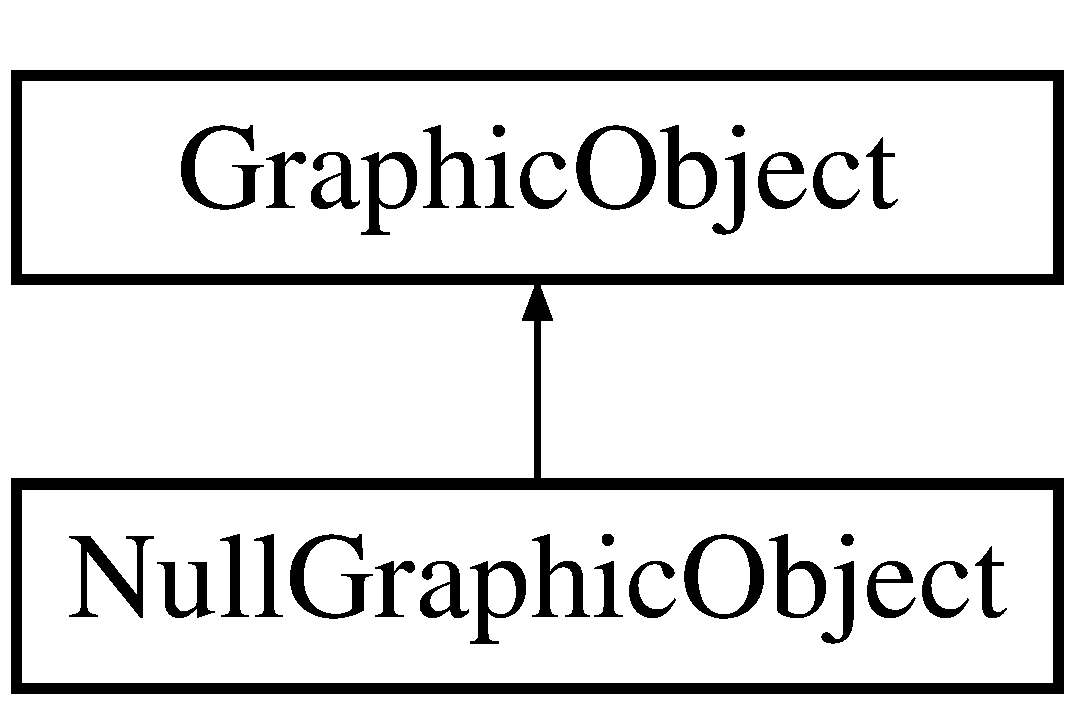
\includegraphics[height=2.000000cm]{classNullGraphicObject}
\end{center}
\end{figure}
\subsection*{Public Member Functions}
\begin{DoxyCompactItemize}
\item 
\hypertarget{classNullGraphicObject_a30a7f189d257cff45556b20a431a4a9c}{}void {\bfseries release} ()\label{classNullGraphicObject_a30a7f189d257cff45556b20a431a4a9c}

\item 
void \hyperlink{classNullGraphicObject_a33c23cd19bac667ad7b1ccbcd9a373d2}{draw} (glm\+::mat4 \&, glm\+::mat4 \&)
\begin{DoxyCompactList}\small\item\em Displays the graphic object. \end{DoxyCompactList}\end{DoxyCompactItemize}
\subsection*{Additional Inherited Members}


\subsection{Detailed Description}
The \hyperlink{classNullGraphicObject}{Null\+Graphic\+Object} class. 

Enables the Null Object pattern for Graphic Object. It means that its methods do nothing and are harmless. 

\subsection{Member Function Documentation}
\hypertarget{classNullGraphicObject_a33c23cd19bac667ad7b1ccbcd9a373d2}{}\index{Null\+Graphic\+Object@{Null\+Graphic\+Object}!draw@{draw}}
\index{draw@{draw}!Null\+Graphic\+Object@{Null\+Graphic\+Object}}
\subsubsection[{draw}]{\setlength{\rightskip}{0pt plus 5cm}void Null\+Graphic\+Object\+::draw (
\begin{DoxyParamCaption}
\item[{glm\+::mat4 \&}]{projection, }
\item[{glm\+::mat4 \&}]{modelview}
\end{DoxyParamCaption}
)\hspace{0.3cm}{\ttfamily [inline]}, {\ttfamily [virtual]}}\label{classNullGraphicObject_a33c23cd19bac667ad7b1ccbcd9a373d2}


Displays the graphic object. 


\begin{DoxyParams}{Parameters}
{\em projection} & The Open\+G\+L projection matrix \\
\hline
{\em modelview} & The Open\+G\+L modelview matrix, which is the product of the model matrix and the view matrix, in this order \\
\hline
\end{DoxyParams}


Implements \hyperlink{classGraphicObject_aacdc39f9e0b36ebb5c815e8bba717d7e}{Graphic\+Object}.



The documentation for this class was generated from the following files\+:\begin{DoxyCompactItemize}
\item 
\hyperlink{GraphicObject_8h}{Graphic\+Object.\+h}\item 
Graphic\+Object.\+cpp\end{DoxyCompactItemize}

\hypertarget{classNullOculus}{}\section{Null\+Oculus Class Reference}
\label{classNullOculus}\index{Null\+Oculus@{Null\+Oculus}}


The \hyperlink{classNullOculus}{Null\+Oculus} class.  




{\ttfamily \#include $<$Oculus.\+h$>$}

Inheritance diagram for Null\+Oculus\+:\begin{figure}[H]
\begin{center}
\leavevmode
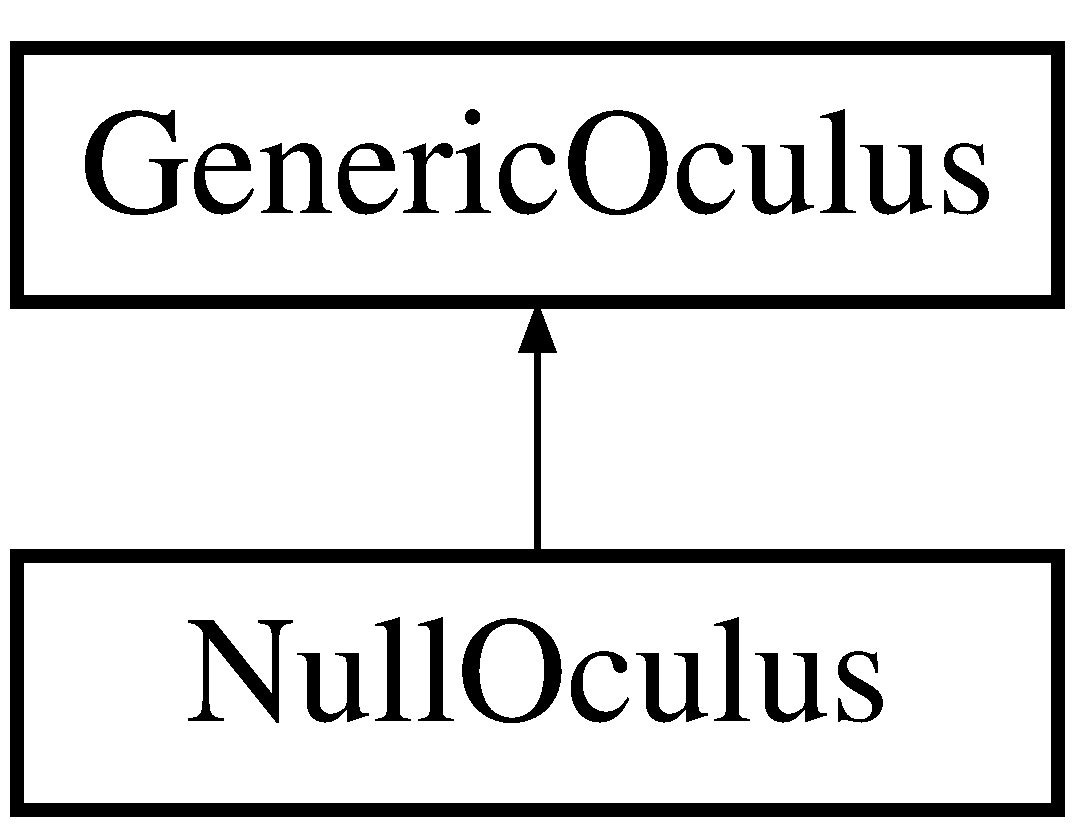
\includegraphics[height=2.000000cm]{classNullOculus}
\end{center}
\end{figure}
\subsection*{Public Member Functions}
\begin{DoxyCompactItemize}
\item 
\hypertarget{classNullOculus_af98f657d9d119a7ed26a43da5ffd0096}{}void {\bfseries render} ()\label{classNullOculus_af98f657d9d119a7ed26a43da5ffd0096}

\end{DoxyCompactItemize}


\subsection{Detailed Description}
The \hyperlink{classNullOculus}{Null\+Oculus} class. 

Part of the Null object pattern 

The documentation for this class was generated from the following files\+:\begin{DoxyCompactItemize}
\item 
\hyperlink{Oculus_8h}{Oculus.\+h}\item 
Oculus.\+cpp\end{DoxyCompactItemize}

\hypertarget{classOculus}{}\section{Oculus$<$ T $>$ Class Template Reference}
\label{classOculus}\index{Oculus$<$ T $>$@{Oculus$<$ T $>$}}


The \hyperlink{classOculus}{Oculus} templated class.  




{\ttfamily \#include $<$Oculus.\+h$>$}

Inheritance diagram for Oculus$<$ T $>$\+:\begin{figure}[H]
\begin{center}
\leavevmode
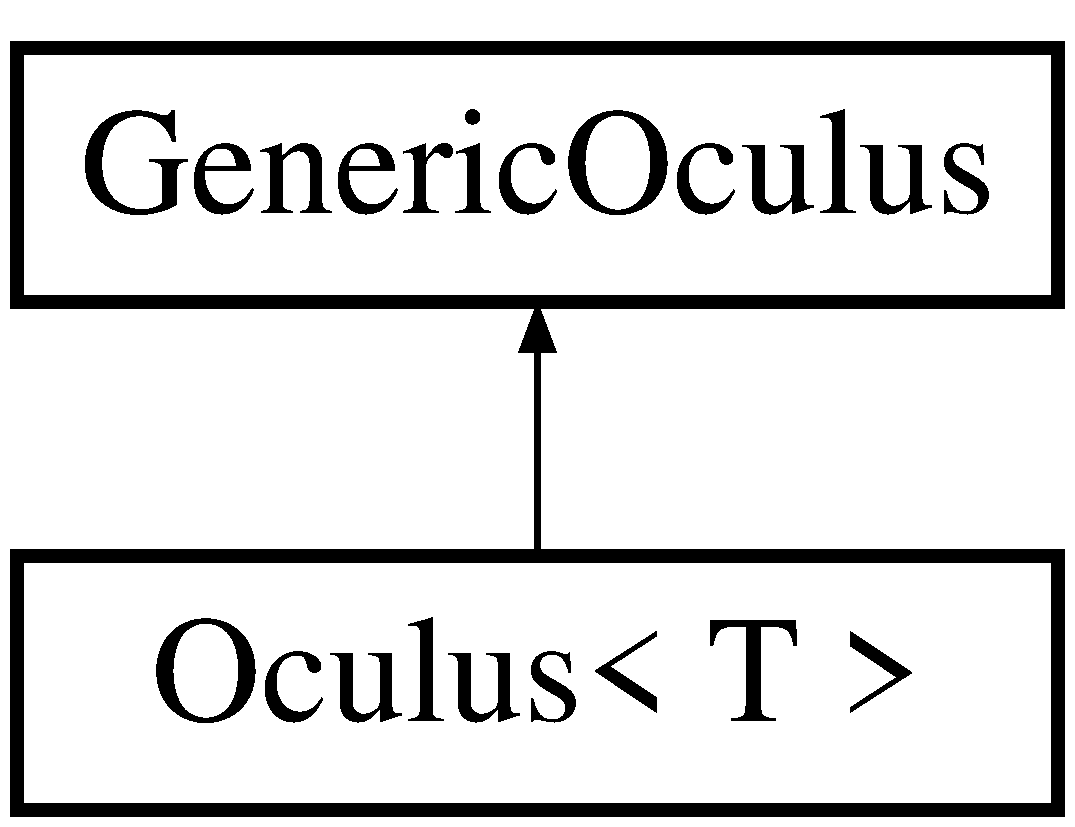
\includegraphics[height=2.000000cm]{classOculus}
\end{center}
\end{figure}
\subsection*{Public Member Functions}
\begin{DoxyCompactItemize}
\item 
\hyperlink{classOculus_a4991461c1a276365ffc8ac9ea8a14451}{Oculus} (T \&scene)
\begin{DoxyCompactList}\small\item\em Constructor. \end{DoxyCompactList}\item 
\hyperlink{classOculus_a042717ce733876a9c2979576d6002107}{$\sim$\+Oculus} ()
\begin{DoxyCompactList}\small\item\em Destructor. \end{DoxyCompactList}\item 
\hypertarget{classOculus_a6c6c91e785d71aff217462ec3e7480e6}{}void \hyperlink{classOculus_a6c6c91e785d71aff217462ec3e7480e6}{render} ()\label{classOculus_a6c6c91e785d71aff217462ec3e7480e6}

\begin{DoxyCompactList}\small\item\em Renders the Open\+G\+L scene with the \hyperlink{classOculus}{Oculus} effects. \end{DoxyCompactList}\item 
bool \hyperlink{classOculus_a35064b5bb6690b448069cb5f632cb29a}{is\+Using\+Debug\+Hmd} ()
\begin{DoxyCompactList}\small\item\em Tells if we are using a debug \hyperlink{classOculus}{Oculus} Rift. \end{DoxyCompactList}\item 
bool \hyperlink{classOculus_a78996f68a93fce8d5b01f6915e1072f2}{is\+Moving} () const 
\begin{DoxyCompactList}\small\item\em Tells if the \hyperlink{classOculus}{Oculus} Rift the moving. \end{DoxyCompactList}\item 
\hypertarget{classOculus_adf5026a36325cfa4e4d2994238586574}{}glm\+::vec3 {\bfseries angles} () const \label{classOculus_adf5026a36325cfa4e4d2994238586574}

\item 
\hypertarget{classOculus_a829fa3c712d6367a5f662942f73adc21}{}void {\bfseries set\+Angles} (const glm\+::vec3 \&angles)\label{classOculus_a829fa3c712d6367a5f662942f73adc21}

\item 
void \hyperlink{classOculus_a60f6bd046dfba11f0d9f3e7277b4a0bb}{get\+Input} ()
\begin{DoxyCompactList}\small\item\em Retrieves the values from the \hyperlink{classOculus}{Oculus} Rift sensors. \end{DoxyCompactList}\end{DoxyCompactItemize}
\subsection*{Protected Member Functions}
\begin{DoxyCompactItemize}
\item 
void \hyperlink{classOculus_a8c20ccdb5b05a138bf7ec4e5efd0c890}{init\+Texture} ()
\begin{DoxyCompactList}\small\item\em Creates the Open\+G\+L texture required for the \hyperlink{classOculus}{Oculus} rendering. \end{DoxyCompactList}\item 
void \hyperlink{classOculus_ae48819d5aca05cf175bbc78327d512cf}{init\+F\+B\+O} ()
\begin{DoxyCompactList}\small\item\em Creates the Frame Buffer Object needed for the \hyperlink{classOculus}{Oculus} rendering. \end{DoxyCompactList}\item 
\hypertarget{classOculus_a774504de4fd7d8b6304d4a1ca7471d28}{}void \hyperlink{classOculus_a774504de4fd7d8b6304d4a1ca7471d28}{init\+Depth\+Buffer} ()\label{classOculus_a774504de4fd7d8b6304d4a1ca7471d28}

\begin{DoxyCompactList}\small\item\em Creates the depth buffer needed for the \hyperlink{classOculus}{Oculus} rendering. \end{DoxyCompactList}\item 
void \hyperlink{classOculus_ae5337c60b8b89c50cfc0ce90d6db2d8f}{set\+Open\+G\+L\+State} ()
\begin{DoxyCompactList}\small\item\em Sets some Open\+G\+L states to adequate values for the \hyperlink{classOculus}{Oculus} rendering. \end{DoxyCompactList}\item 
void \hyperlink{classOculus_add30e49061a9ec8a5676f9be24e8eec7}{set\+Cfg} ()
\begin{DoxyCompactList}\small\item\em Sets the \hyperlink{classOculus}{Oculus} S\+D\+K configuration to adequate values for the \hyperlink{classOculus}{Oculus} rendering. \end{DoxyCompactList}\item 
\hypertarget{classOculus_a5e1def14eace52ef4f62c263888c5fd2}{}void \hyperlink{classOculus_a5e1def14eace52ef4f62c263888c5fd2}{set\+Eye\+Texture} ()\label{classOculus_a5e1def14eace52ef4f62c263888c5fd2}

\begin{DoxyCompactList}\small\item\em Sets the \hyperlink{classOculus}{Oculus} S\+D\+K texture configuration to adequate values for the \hyperlink{classOculus}{Oculus} rendering. \end{DoxyCompactList}\item 
void \hyperlink{classOculus_a21273c2c3dd1e2d4b9d113cac0d72ec3}{compute\+Sizes} ()
\begin{DoxyCompactList}\small\item\em Computes the texture size. \end{DoxyCompactList}\item 
\hypertarget{classOculus_a4a26271c5d8d4f7350bb7b85c829dd97}{}glm\+::vec3 {\bfseries d\+Angles} () const \label{classOculus_a4a26271c5d8d4f7350bb7b85c829dd97}

\end{DoxyCompactItemize}
\subsection*{Protected Attributes}
\begin{DoxyCompactItemize}
\item 
T \& \hyperlink{classOculus_a8a88e3b8bb25831c6fb001fbdac6b45b}{scene\+\_\+}
\begin{DoxyCompactList}\small\item\em The generic Open\+G\+L scene. \end{DoxyCompactList}\item 
\hypertarget{classOculus_a5e97a6716ef4b94b87eb2a0452e32eb4}{}G\+Luint \hyperlink{classOculus_a5e97a6716ef4b94b87eb2a0452e32eb4}{texture\+Id\+\_\+}\label{classOculus_a5e97a6716ef4b94b87eb2a0452e32eb4}

\begin{DoxyCompactList}\small\item\em The id of the Open\+G\+L texture used in the \hyperlink{classOculus}{Oculus} rendering. \end{DoxyCompactList}\item 
\hypertarget{classOculus_a3918541266c72f1bb3f84225edc37e95}{}G\+Luint \hyperlink{classOculus_a3918541266c72f1bb3f84225edc37e95}{F\+B\+O\+Id\+\_\+}\label{classOculus_a3918541266c72f1bb3f84225edc37e95}

\begin{DoxyCompactList}\small\item\em The id of the Open\+G\+L Frame Buffer Object used in the \hyperlink{classOculus}{Oculus} rendering. \end{DoxyCompactList}\item 
\hypertarget{classOculus_a420de1ed9815712680893b1a61d90dfc}{}G\+Luint \hyperlink{classOculus_a420de1ed9815712680893b1a61d90dfc}{depth\+Buffer\+Id\+\_\+}\label{classOculus_a420de1ed9815712680893b1a61d90dfc}

\begin{DoxyCompactList}\small\item\em The id of the Open\+G\+L depth buffer used in the \hyperlink{classOculus}{Oculus} rendering. \end{DoxyCompactList}\item 
ovr\+Hmd \hyperlink{classOculus_a27b4553058255871d50e941d67de5374}{hmd\+\_\+}
\begin{DoxyCompactList}\small\item\em The \hyperlink{classOculus}{Oculus} Rift. \end{DoxyCompactList}\item 
ovr\+Hmd\+Desc \hyperlink{classOculus_aaca119fa80d400cb78ce54b69bc39081}{hmd\+Desc\+\_\+}
\begin{DoxyCompactList}\small\item\em The description of the \hyperlink{classOculus}{Oculus} Rift. \end{DoxyCompactList}\item 
ovr\+Eye\+Render\+Desc \hyperlink{classOculus_a6697ef38f95623320ff9e78cc2474567}{eye\+Render\+Desc\+\_\+} \mbox{[}2\mbox{]}
\begin{DoxyCompactList}\small\item\em The description of each eye. \end{DoxyCompactList}\item 
\hypertarget{classOculus_ac041c19b742d76349275583e75dd651a}{}ovr\+G\+L\+Texture \hyperlink{classOculus_ac041c19b742d76349275583e75dd651a}{eye\+Texture\+\_\+} \mbox{[}2\mbox{]}\label{classOculus_ac041c19b742d76349275583e75dd651a}

\begin{DoxyCompactList}\small\item\em The texture of each eye. \end{DoxyCompactList}\item 
\hypertarget{classOculus_a13e8cb827b31c4e96472117488bc04a2}{}ovr\+Fov\+Port \hyperlink{classOculus_a13e8cb827b31c4e96472117488bc04a2}{eye\+Fov\+\_\+} \mbox{[}2\mbox{]}\label{classOculus_a13e8cb827b31c4e96472117488bc04a2}

\begin{DoxyCompactList}\small\item\em The Field of View of each eye. \end{DoxyCompactList}\item 
\hypertarget{classOculus_ab1c10f5b1431c8c13507938e6de46f44}{}ovr\+G\+L\+Config \hyperlink{classOculus_ab1c10f5b1431c8c13507938e6de46f44}{cfg\+\_\+}\label{classOculus_ab1c10f5b1431c8c13507938e6de46f44}

\begin{DoxyCompactList}\small\item\em The configuration for the Open\+G\+L \hyperlink{classOculus}{Oculus} rendering. \end{DoxyCompactList}\item 
\hypertarget{classOculus_a944e263e7aee6b568b69211896e05365}{}ovr\+Sizei \hyperlink{classOculus_a944e263e7aee6b568b69211896e05365}{window\+Size\+\_\+}\label{classOculus_a944e263e7aee6b568b69211896e05365}

\begin{DoxyCompactList}\small\item\em The dimensions of the window. \end{DoxyCompactList}\item 
\hypertarget{classOculus_a33ff393c9f149ea6e559629c6de3fb9c}{}ovr\+Sizei \hyperlink{classOculus_a33ff393c9f149ea6e559629c6de3fb9c}{texture\+Size\+Left\+\_\+}\label{classOculus_a33ff393c9f149ea6e559629c6de3fb9c}

\begin{DoxyCompactList}\small\item\em The dimensions of the texture that the left eye can see. \end{DoxyCompactList}\item 
\hypertarget{classOculus_a742ac672ac7679c1d6b03a5fe2595f96}{}ovr\+Sizei \hyperlink{classOculus_a742ac672ac7679c1d6b03a5fe2595f96}{texture\+Size\+Right\+\_\+}\label{classOculus_a742ac672ac7679c1d6b03a5fe2595f96}

\begin{DoxyCompactList}\small\item\em The dimensions of the texture that the right eye can see. \end{DoxyCompactList}\item 
\hypertarget{classOculus_a079b9f2a9887330a4001e42cac663a18}{}ovr\+Sizei \hyperlink{classOculus_a079b9f2a9887330a4001e42cac663a18}{texture\+Size\+\_\+}\label{classOculus_a079b9f2a9887330a4001e42cac663a18}

\begin{DoxyCompactList}\small\item\em The dimensions of the texture overall. \end{DoxyCompactList}\item 
\hypertarget{classOculus_a3dc18febcca74ef3ed83276945bb6395}{}ovr\+Frame\+Timing \hyperlink{classOculus_a3dc18febcca74ef3ed83276945bb6395}{frame\+Timing\+\_\+}\label{classOculus_a3dc18febcca74ef3ed83276945bb6395}

\begin{DoxyCompactList}\small\item\em Time variable used by the sensor and the predication tool. \end{DoxyCompactList}\item 
\hypertarget{classOculus_a37a433aa3b8444d0a5438073a7d7b5b4}{}ovr\+Sensor\+State \hyperlink{classOculus_a37a433aa3b8444d0a5438073a7d7b5b4}{sensor\+State\+\_\+}\label{classOculus_a37a433aa3b8444d0a5438073a7d7b5b4}

\begin{DoxyCompactList}\small\item\em The \hyperlink{classOculus}{Oculus} Rift sensors. \end{DoxyCompactList}\item 
\hypertarget{classOculus_a99c5e2751f5e1aaf42d177b0d36ac62d}{}glm\+::vec3 \hyperlink{classOculus_a99c5e2751f5e1aaf42d177b0d36ac62d}{angles\+\_\+}\label{classOculus_a99c5e2751f5e1aaf42d177b0d36ac62d}

\begin{DoxyCompactList}\small\item\em The \hyperlink{classOculus}{Oculus} Rift angular position. \end{DoxyCompactList}\item 
\hypertarget{classOculus_a3065d87c9d010aaf83822c8414b680c4}{}glm\+::vec3 \hyperlink{classOculus_a3065d87c9d010aaf83822c8414b680c4}{d\+Angles\+\_\+}\label{classOculus_a3065d87c9d010aaf83822c8414b680c4}

\begin{DoxyCompactList}\small\item\em The \hyperlink{classOculus}{Oculus} Rift angular position variation. \end{DoxyCompactList}\item 
\hypertarget{classOculus_ae5ae5f7bf69f57f9d40a6792843fed87}{}int \hyperlink{classOculus_ae5ae5f7bf69f57f9d40a6792843fed87}{distortion\+Caps\+\_\+}\label{classOculus_ae5ae5f7bf69f57f9d40a6792843fed87}

\begin{DoxyCompactList}\small\item\em Flag used for the \hyperlink{classOculus}{Oculus} rendering configuration. \end{DoxyCompactList}\item 
\hypertarget{classOculus_aeef8b424f3fc4d181b18f01c15809e25}{}bool \hyperlink{classOculus_aeef8b424f3fc4d181b18f01c15809e25}{using\+Debug\+Hmd\+\_\+}\label{classOculus_aeef8b424f3fc4d181b18f01c15809e25}

\begin{DoxyCompactList}\small\item\em Boolean indicating if we are using a debug \hyperlink{classOculus}{Oculus} Rift. \end{DoxyCompactList}\item 
bool \hyperlink{classOculus_a526eb65105ddf30005f1a14fd9325e6c}{multisample\+Enabled\+\_\+}
\begin{DoxyCompactList}\small\item\em Boolean indicating if the \hyperlink{classOculus}{Oculus} rendering is multisampled. \end{DoxyCompactList}\end{DoxyCompactItemize}
\subsection*{Static Protected Attributes}
\begin{DoxyCompactItemize}
\item 
static bool \hyperlink{classOculus_a56f59153d62ca8802b7573abd6059967}{already\+Created} = false
\begin{DoxyCompactList}\small\item\em Boolean that shows whether or not an instance has already been created. \end{DoxyCompactList}\end{DoxyCompactItemize}


\subsection{Detailed Description}
\subsubsection*{template$<$class T$>$class Oculus$<$ T $>$}

The \hyperlink{classOculus}{Oculus} templated class. 

It is a singleton to avoid initializing/releasing the \hyperlink{classOculus}{Oculus} S\+D\+K multiple times. The template argument is the type of the Ope\+G\+L scene we render. 

\subsection{Constructor \& Destructor Documentation}
\hypertarget{classOculus_a4991461c1a276365ffc8ac9ea8a14451}{}\index{Oculus@{Oculus}!Oculus@{Oculus}}
\index{Oculus@{Oculus}!Oculus@{Oculus}}
\subsubsection[{Oculus}]{\setlength{\rightskip}{0pt plus 5cm}template$<$class T $>$ {\bf Oculus}$<$ T $>$\+::{\bf Oculus} (
\begin{DoxyParamCaption}
\item[{T \&}]{scene}
\end{DoxyParamCaption}
)\hspace{0.3cm}{\ttfamily [inline]}}\label{classOculus_a4991461c1a276365ffc8ac9ea8a14451}


Constructor. 

Initializes the \hyperlink{classOculus}{Oculus} S\+D\+K, creates a debug \hyperlink{classOculus}{Oculus} Rift if none is connected, and starts the sensors. 
\begin{DoxyParams}{Parameters}
{\em scene} & The Open\+G\+L scene that contains the objects render \\
\hline
\end{DoxyParams}
\hypertarget{classOculus_a042717ce733876a9c2979576d6002107}{}\index{Oculus@{Oculus}!````~Oculus@{$\sim$\+Oculus}}
\index{````~Oculus@{$\sim$\+Oculus}!Oculus@{Oculus}}
\subsubsection[{$\sim$\+Oculus}]{\setlength{\rightskip}{0pt plus 5cm}template$<$class T $>$ {\bf Oculus}$<$ T $>$\+::$\sim${\bf Oculus} (
\begin{DoxyParamCaption}
{}
\end{DoxyParamCaption}
)\hspace{0.3cm}{\ttfamily [inline]}}\label{classOculus_a042717ce733876a9c2979576d6002107}


Destructor. 

Releases the \hyperlink{classOculus}{Oculus} S\+D\+K and the Open\+G\+L resources required for the \hyperlink{classOculus}{Oculus} rendering 

\subsection{Member Function Documentation}
\hypertarget{classOculus_a21273c2c3dd1e2d4b9d113cac0d72ec3}{}\index{Oculus@{Oculus}!compute\+Sizes@{compute\+Sizes}}
\index{compute\+Sizes@{compute\+Sizes}!Oculus@{Oculus}}
\subsubsection[{compute\+Sizes}]{\setlength{\rightskip}{0pt plus 5cm}template$<$class T $>$ void {\bf Oculus}$<$ T $>$\+::compute\+Sizes (
\begin{DoxyParamCaption}
{}
\end{DoxyParamCaption}
)\hspace{0.3cm}{\ttfamily [inline]}, {\ttfamily [protected]}}\label{classOculus_a21273c2c3dd1e2d4b9d113cac0d72ec3}


Computes the texture size. 

This computation depends on the window dimensions. The optimal dimensions are 1280$\ast$800, which is the \hyperlink{classOculus}{Oculus} resolution \begin{DoxyWarning}{Warning}
Other resolutions and window resizing have not been tested but should work just fine 
\end{DoxyWarning}
\hypertarget{classOculus_a60f6bd046dfba11f0d9f3e7277b4a0bb}{}\index{Oculus@{Oculus}!get\+Input@{get\+Input}}
\index{get\+Input@{get\+Input}!Oculus@{Oculus}}
\subsubsection[{get\+Input}]{\setlength{\rightskip}{0pt plus 5cm}template$<$class T $>$ void {\bf Oculus}$<$ T $>$\+::get\+Input (
\begin{DoxyParamCaption}
{}
\end{DoxyParamCaption}
)\hspace{0.3cm}{\ttfamily [inline]}, {\ttfamily [virtual]}}\label{classOculus_a60f6bd046dfba11f0d9f3e7277b4a0bb}


Retrieves the values from the \hyperlink{classOculus}{Oculus} Rift sensors. 

It gets the current angular position from the sensors and the prediction tool, and stores the old angular position. \begin{DoxyWarning}{Warning}
The angles from the sensors are in radians and Open\+G\+L expects angles in degrees, hence the required conversion 

If no \hyperlink{classOculus}{Oculus} Rift is connected and we had to create a debug one, there are no values to be retrieved\+: We use the mouse position. 
\end{DoxyWarning}


Reimplemented from \hyperlink{classGenericOculus}{Generic\+Oculus}.

\hypertarget{classOculus_ae48819d5aca05cf175bbc78327d512cf}{}\index{Oculus@{Oculus}!init\+F\+B\+O@{init\+F\+B\+O}}
\index{init\+F\+B\+O@{init\+F\+B\+O}!Oculus@{Oculus}}
\subsubsection[{init\+F\+B\+O}]{\setlength{\rightskip}{0pt plus 5cm}template$<$class T $>$ void {\bf Oculus}$<$ T $>$\+::init\+F\+B\+O (
\begin{DoxyParamCaption}
{}
\end{DoxyParamCaption}
)\hspace{0.3cm}{\ttfamily [inline]}, {\ttfamily [protected]}}\label{classOculus_ae48819d5aca05cf175bbc78327d512cf}


Creates the Frame Buffer Object needed for the \hyperlink{classOculus}{Oculus} rendering. 

The \hyperlink{classOculus}{Oculus} rendering uses this F\+B\+O to send the texture to the graphic card \hypertarget{classOculus_a8c20ccdb5b05a138bf7ec4e5efd0c890}{}\index{Oculus@{Oculus}!init\+Texture@{init\+Texture}}
\index{init\+Texture@{init\+Texture}!Oculus@{Oculus}}
\subsubsection[{init\+Texture}]{\setlength{\rightskip}{0pt plus 5cm}template$<$class T $>$ void {\bf Oculus}$<$ T $>$\+::init\+Texture (
\begin{DoxyParamCaption}
{}
\end{DoxyParamCaption}
)\hspace{0.3cm}{\ttfamily [inline]}, {\ttfamily [protected]}}\label{classOculus_a8c20ccdb5b05a138bf7ec4e5efd0c890}


Creates the Open\+G\+L texture required for the \hyperlink{classOculus}{Oculus} rendering. 

The \hyperlink{classOculus}{Oculus} rendering makes under the hood a double (for each eye) render to texture of the scene and then displays this texture to the screen, hence the big size of the texture. \hypertarget{classOculus_a78996f68a93fce8d5b01f6915e1072f2}{}\index{Oculus@{Oculus}!is\+Moving@{is\+Moving}}
\index{is\+Moving@{is\+Moving}!Oculus@{Oculus}}
\subsubsection[{is\+Moving}]{\setlength{\rightskip}{0pt plus 5cm}template$<$class T $>$ bool {\bf Oculus}$<$ T $>$\+::is\+Moving (
\begin{DoxyParamCaption}
{}
\end{DoxyParamCaption}
) const\hspace{0.3cm}{\ttfamily [inline]}, {\ttfamily [virtual]}}\label{classOculus_a78996f68a93fce8d5b01f6915e1072f2}


Tells if the \hyperlink{classOculus}{Oculus} Rift the moving. 

It compares the current angular position with the previous angular position \begin{DoxyReturn}{Returns}
true if the \hyperlink{classOculus}{Oculus} Rift if moving, else false 
\end{DoxyReturn}


Reimplemented from \hyperlink{classGenericOculus}{Generic\+Oculus}.

\hypertarget{classOculus_a35064b5bb6690b448069cb5f632cb29a}{}\index{Oculus@{Oculus}!is\+Using\+Debug\+Hmd@{is\+Using\+Debug\+Hmd}}
\index{is\+Using\+Debug\+Hmd@{is\+Using\+Debug\+Hmd}!Oculus@{Oculus}}
\subsubsection[{is\+Using\+Debug\+Hmd}]{\setlength{\rightskip}{0pt plus 5cm}template$<$class T $>$ bool {\bf Oculus}$<$ T $>$\+::is\+Using\+Debug\+Hmd (
\begin{DoxyParamCaption}
{}
\end{DoxyParamCaption}
)\hspace{0.3cm}{\ttfamily [inline]}, {\ttfamily [virtual]}}\label{classOculus_a35064b5bb6690b448069cb5f632cb29a}


Tells if we are using a debug \hyperlink{classOculus}{Oculus} Rift. 

\begin{DoxyReturn}{Returns}
true if no \hyperlink{classOculus}{Oculus} Rift is connected and we had to create a debug one, else false 
\end{DoxyReturn}


Reimplemented from \hyperlink{classGenericOculus}{Generic\+Oculus}.

\hypertarget{classOculus_add30e49061a9ec8a5676f9be24e8eec7}{}\index{Oculus@{Oculus}!set\+Cfg@{set\+Cfg}}
\index{set\+Cfg@{set\+Cfg}!Oculus@{Oculus}}
\subsubsection[{set\+Cfg}]{\setlength{\rightskip}{0pt plus 5cm}template$<$class T $>$ void {\bf Oculus}$<$ T $>$\+::set\+Cfg (
\begin{DoxyParamCaption}
{}
\end{DoxyParamCaption}
)\hspace{0.3cm}{\ttfamily [inline]}, {\ttfamily [protected]}}\label{classOculus_add30e49061a9ec8a5676f9be24e8eec7}


Sets the \hyperlink{classOculus}{Oculus} S\+D\+K configuration to adequate values for the \hyperlink{classOculus}{Oculus} rendering. 

\begin{DoxyWarning}{Warning}
The Windows and O\+S\+X modes have not been tested but should work just fine 
\end{DoxyWarning}
\hypertarget{classOculus_ae5337c60b8b89c50cfc0ce90d6db2d8f}{}\index{Oculus@{Oculus}!set\+Open\+G\+L\+State@{set\+Open\+G\+L\+State}}
\index{set\+Open\+G\+L\+State@{set\+Open\+G\+L\+State}!Oculus@{Oculus}}
\subsubsection[{set\+Open\+G\+L\+State}]{\setlength{\rightskip}{0pt plus 5cm}template$<$class T $>$ void {\bf Oculus}$<$ T $>$\+::set\+Open\+G\+L\+State (
\begin{DoxyParamCaption}
{}
\end{DoxyParamCaption}
)\hspace{0.3cm}{\ttfamily [inline]}, {\ttfamily [protected]}}\label{classOculus_ae5337c60b8b89c50cfc0ce90d6db2d8f}


Sets some Open\+G\+L states to adequate values for the \hyperlink{classOculus}{Oculus} rendering. 

\begin{DoxyWarning}{Warning}
The multisample value does not seem the be taken into account by the \hyperlink{classOculus}{Oculus} S\+D\+K as of yet and the \hyperlink{classOculus}{Oculus} rendering seems unchanged 
\end{DoxyWarning}


\subsection{Member Data Documentation}
\hypertarget{classOculus_a56f59153d62ca8802b7573abd6059967}{}\index{Oculus@{Oculus}!already\+Created@{already\+Created}}
\index{already\+Created@{already\+Created}!Oculus@{Oculus}}
\subsubsection[{already\+Created}]{\setlength{\rightskip}{0pt plus 5cm}template$<$class T $>$ bool {\bf Oculus}$<$ T $>$\+::already\+Created = false\hspace{0.3cm}{\ttfamily [static]}, {\ttfamily [protected]}}\label{classOculus_a56f59153d62ca8802b7573abd6059967}


Boolean that shows whether or not an instance has already been created. 

Part of the Singleton Pattern \hypertarget{classOculus_a6697ef38f95623320ff9e78cc2474567}{}\index{Oculus@{Oculus}!eye\+Render\+Desc\+\_\+@{eye\+Render\+Desc\+\_\+}}
\index{eye\+Render\+Desc\+\_\+@{eye\+Render\+Desc\+\_\+}!Oculus@{Oculus}}
\subsubsection[{eye\+Render\+Desc\+\_\+}]{\setlength{\rightskip}{0pt plus 5cm}template$<$class T $>$ ovr\+Eye\+Render\+Desc {\bf Oculus}$<$ T $>$\+::eye\+Render\+Desc\+\_\+\mbox{[}2\mbox{]}\hspace{0.3cm}{\ttfamily [protected]}}\label{classOculus_a6697ef38f95623320ff9e78cc2474567}


The description of each eye. 

Contains lots of values like dimensions, wether it is the left or right eye, etc. \hypertarget{classOculus_a27b4553058255871d50e941d67de5374}{}\index{Oculus@{Oculus}!hmd\+\_\+@{hmd\+\_\+}}
\index{hmd\+\_\+@{hmd\+\_\+}!Oculus@{Oculus}}
\subsubsection[{hmd\+\_\+}]{\setlength{\rightskip}{0pt plus 5cm}template$<$class T $>$ ovr\+Hmd {\bf Oculus}$<$ T $>$\+::hmd\+\_\+\hspace{0.3cm}{\ttfamily [protected]}}\label{classOculus_a27b4553058255871d50e941d67de5374}


The \hyperlink{classOculus}{Oculus} Rift. 

If no \hyperlink{classOculus}{Oculus} Rift is connected, a debug one is created. The last does not have proper sensors. \hypertarget{classOculus_aaca119fa80d400cb78ce54b69bc39081}{}\index{Oculus@{Oculus}!hmd\+Desc\+\_\+@{hmd\+Desc\+\_\+}}
\index{hmd\+Desc\+\_\+@{hmd\+Desc\+\_\+}!Oculus@{Oculus}}
\subsubsection[{hmd\+Desc\+\_\+}]{\setlength{\rightskip}{0pt plus 5cm}template$<$class T $>$ ovr\+Hmd\+Desc {\bf Oculus}$<$ T $>$\+::hmd\+Desc\+\_\+\hspace{0.3cm}{\ttfamily [protected]}}\label{classOculus_aaca119fa80d400cb78ce54b69bc39081}


The description of the \hyperlink{classOculus}{Oculus} Rift. 

Contains lots of values like inter-\/pupillary distance, resolution, etc \hypertarget{classOculus_a526eb65105ddf30005f1a14fd9325e6c}{}\index{Oculus@{Oculus}!multisample\+Enabled\+\_\+@{multisample\+Enabled\+\_\+}}
\index{multisample\+Enabled\+\_\+@{multisample\+Enabled\+\_\+}!Oculus@{Oculus}}
\subsubsection[{multisample\+Enabled\+\_\+}]{\setlength{\rightskip}{0pt plus 5cm}template$<$class T $>$ bool {\bf Oculus}$<$ T $>$\+::multisample\+Enabled\+\_\+\hspace{0.3cm}{\ttfamily [protected]}}\label{classOculus_a526eb65105ddf30005f1a14fd9325e6c}


Boolean indicating if the \hyperlink{classOculus}{Oculus} rendering is multisampled. 

\begin{DoxyWarning}{Warning}
The \hyperlink{classOculus}{Oculus} S\+D\+K does not seem to take this variable into account as of yet 
\end{DoxyWarning}
\hypertarget{classOculus_a8a88e3b8bb25831c6fb001fbdac6b45b}{}\index{Oculus@{Oculus}!scene\+\_\+@{scene\+\_\+}}
\index{scene\+\_\+@{scene\+\_\+}!Oculus@{Oculus}}
\subsubsection[{scene\+\_\+}]{\setlength{\rightskip}{0pt plus 5cm}template$<$class T $>$ T\& {\bf Oculus}$<$ T $>$\+::scene\+\_\+\hspace{0.3cm}{\ttfamily [protected]}}\label{classOculus_a8a88e3b8bb25831c6fb001fbdac6b45b}


The generic Open\+G\+L scene. 

\hyperlink{classOculus}{Oculus} is a templated class and its only argument is the type of {\itshape scene}. The only requirement is that scene has a method {\itshape render}, wich takes as argument the modelview matrix and the projection matrix. 

The documentation for this class was generated from the following file\+:\begin{DoxyCompactItemize}
\item 
\hyperlink{Oculus_8h}{Oculus.\+h}\end{DoxyCompactItemize}

\hypertarget{classPlane}{}\section{Plane Class Reference}
\label{classPlane}\index{Plane@{Plane}}


The \hyperlink{classPlane}{Plane} class.  




{\ttfamily \#include $<$Plane.\+h$>$}

Inheritance diagram for Plane\+:\begin{figure}[H]
\begin{center}
\leavevmode
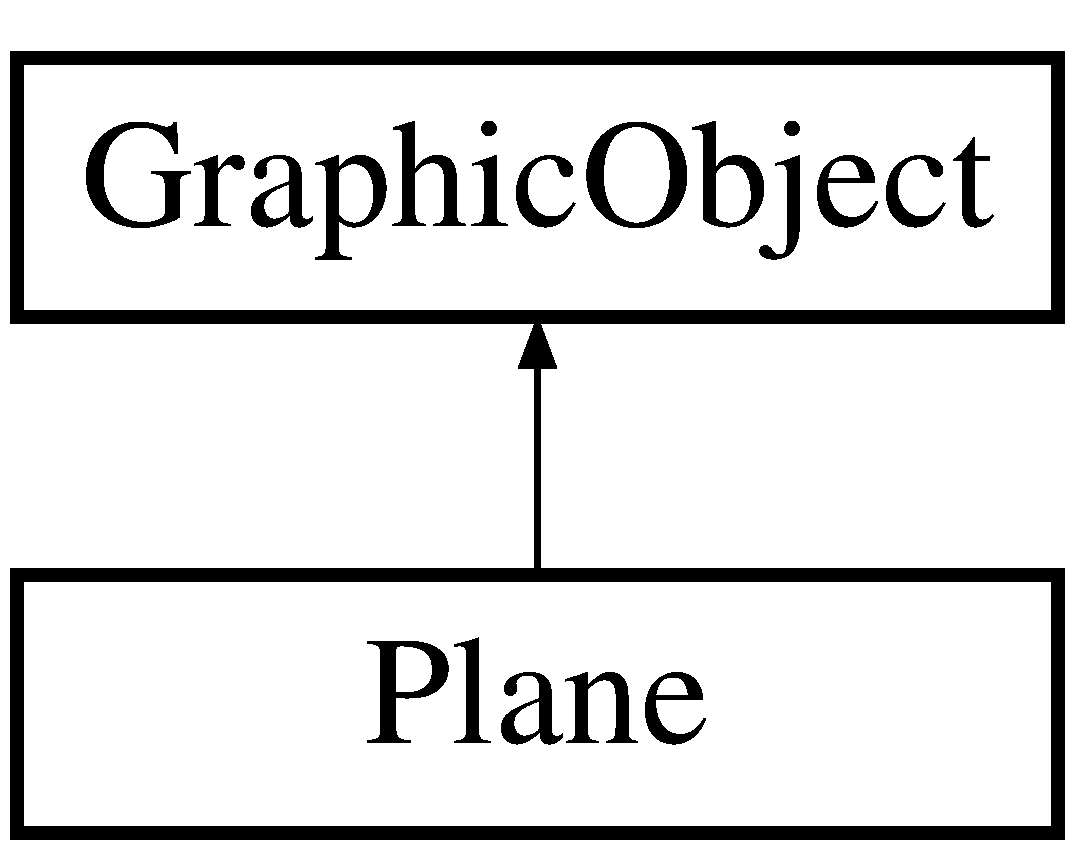
\includegraphics[height=2.000000cm]{classPlane}
\end{center}
\end{figure}
\subsection*{Public Member Functions}
\begin{DoxyCompactItemize}
\item 
\hypertarget{classPlane_a63651155afec5a2c904a80ec9b87335c}{}{\bfseries Plane} (float x, float y, float z, float width, float height, float repeat\+Width, float repeat\+Height, std\+::string const \&vertex\+Shader, std\+::string const \&frag\+Shader, std\+::string const \&texture)\label{classPlane_a63651155afec5a2c904a80ec9b87335c}

\item 
void \hyperlink{classPlane_ac046dce6b4226e86fbcaf850fa7e30fd}{draw} (glm\+::mat4 \&projection, glm\+::mat4 \&modelview)
\begin{DoxyCompactList}\small\item\em Displays the graphic object. \end{DoxyCompactList}\item 
\hypertarget{classPlane_a6dc72a0c50fad122fabfbd0bd73e6b75}{}virtual void {\bfseries load} ()\label{classPlane_a6dc72a0c50fad122fabfbd0bd73e6b75}

\item 
\hypertarget{classPlane_a678ea174d88d8615e89d2b5e03f9b537}{}int {\bfseries nb\+Texture\+Bytes} ()\label{classPlane_a678ea174d88d8615e89d2b5e03f9b537}

\end{DoxyCompactItemize}
\subsection*{Protected Attributes}
\begin{DoxyCompactItemize}
\item 
\hypertarget{classPlane_a876de2b83e6c8c6d3b36c8bccee28bd0}{}std\+::vector$<$ float $>$ {\bfseries texture\+Coord\+\_\+}\label{classPlane_a876de2b83e6c8c6d3b36c8bccee28bd0}

\item 
\hypertarget{classPlane_ae18aab7f950602d3d1ee3d30405dfe11}{}std\+::shared\+\_\+ptr$<$ \hyperlink{classTexture}{Texture} $>$ {\bfseries texture\+\_\+}\label{classPlane_ae18aab7f950602d3d1ee3d30405dfe11}

\end{DoxyCompactItemize}


\subsection{Detailed Description}
The \hyperlink{classPlane}{Plane} class. 

A plane is a simple flat 2 dimensional surface. Uses the Flyweight pattern with a shared texture pool 

\subsection{Member Function Documentation}
\hypertarget{classPlane_ac046dce6b4226e86fbcaf850fa7e30fd}{}\index{Plane@{Plane}!draw@{draw}}
\index{draw@{draw}!Plane@{Plane}}
\subsubsection[{draw}]{\setlength{\rightskip}{0pt plus 5cm}void Plane\+::draw (
\begin{DoxyParamCaption}
\item[{glm\+::mat4 \&}]{projection, }
\item[{glm\+::mat4 \&}]{modelview}
\end{DoxyParamCaption}
)\hspace{0.3cm}{\ttfamily [virtual]}}\label{classPlane_ac046dce6b4226e86fbcaf850fa7e30fd}


Displays the graphic object. 


\begin{DoxyParams}{Parameters}
{\em projection} & The Open\+G\+L projection matrix \\
\hline
{\em modelview} & The Open\+G\+L modelview matrix, which is the product of the model matrix and the view matrix, in this order \\
\hline
\end{DoxyParams}


Implements \hyperlink{classGraphicObject_aacdc39f9e0b36ebb5c815e8bba717d7e}{Graphic\+Object}.



The documentation for this class was generated from the following files\+:\begin{DoxyCompactItemize}
\item 
\hyperlink{Plane_8h}{Plane.\+h}\item 
Plane.\+cpp\end{DoxyCompactItemize}

\hypertarget{classScene}{}\section{Scene Class Reference}
\label{classScene}\index{Scene@{Scene}}


The \hyperlink{classScene}{Scene} class.  




{\ttfamily \#include $<$Scene.\+h$>$}

\subsection*{Public Member Functions}
\begin{DoxyCompactItemize}
\item 
\hypertarget{classScene_aeb61892e50f410db3fd84be5037a1e3c}{}{\bfseries Scene} (std\+::string window\+Title, int window\+Width, int window\+Height, bool oculus\+Render, bool fullscreen, std\+::string texture\+Name, unsigned long objects\+Count, int size, int octant\+Size, int octants\+Drawn\+Count, std\+::string filename, int random\+Percentage, int clustering\+Percentage, bool is\+Multi\+Thread, bool render\+Type\+Simplified)\label{classScene_aeb61892e50f410db3fd84be5037a1e3c}

\item 
\hypertarget{classScene_ab81ad242d6c35a24cfffb693b343cd20}{}void \hyperlink{classScene_ab81ad242d6c35a24cfffb693b343cd20}{main\+Loop} ()\label{classScene_ab81ad242d6c35a24cfffb693b343cd20}

\begin{DoxyCompactList}\small\item\em The main loop of the application. \end{DoxyCompactList}\item 
\hypertarget{classScene_ae0a213f3b0461622c7a5124362975603}{}void \hyperlink{classScene_ae0a213f3b0461622c7a5124362975603}{main\+Loop\+Test} ()\label{classScene_ae0a213f3b0461622c7a5124362975603}

\begin{DoxyCompactList}\small\item\em The main loop to test the application. \end{DoxyCompactList}\item 
\hypertarget{classScene_a4ddf2d16f371ee9533b3faf1dd5ddfb1}{}void \hyperlink{classScene_a4ddf2d16f371ee9533b3faf1dd5ddfb1}{render} ()\label{classScene_a4ddf2d16f371ee9533b3faf1dd5ddfb1}

\begin{DoxyCompactList}\small\item\em The graphical rendering. \end{DoxyCompactList}\item 
void \hyperlink{classScene_a693d39c8c9c53dfd6307fcd3293506da}{render} (glm\+::mat4 \&M\+V, glm\+::mat4 \&proj)
\begin{DoxyCompactList}\small\item\em The graphical rendering. \end{DoxyCompactList}\item 
\hypertarget{classScene_ae20240e6c189eb8088ae92b4be5625f8}{}S\+D\+L\+\_\+\+Window $\ast$ {\bfseries window} () const \label{classScene_ae20240e6c189eb8088ae92b4be5625f8}

\item 
\hypertarget{classScene_a9ce2dab07ddcb400a08953f9faebfdf5}{}int {\bfseries window\+Width} () const \label{classScene_a9ce2dab07ddcb400a08953f9faebfdf5}

\item 
\hypertarget{classScene_acf77d9dc5f53f98f506e1ffc0636662d}{}void {\bfseries set\+Window\+Width} (int window\+Width)\label{classScene_acf77d9dc5f53f98f506e1ffc0636662d}

\item 
\hypertarget{classScene_ad899521bb92f8a0818d263e255bde87d}{}int {\bfseries window\+Height} () const \label{classScene_ad899521bb92f8a0818d263e255bde87d}

\item 
\hypertarget{classScene_a8e81e065002b9a95c575b94f9129bb35}{}void {\bfseries set\+Window\+Height} (int window\+Height)\label{classScene_a8e81e065002b9a95c575b94f9129bb35}

\item 
bool \hyperlink{classScene_aec8cd9d85f671a8c2c1f45b373fc90b7}{is\+Random\+Point} (int n)
\begin{DoxyCompactList}\small\item\em is\+Random\+Point \end{DoxyCompactList}\end{DoxyCompactItemize}


\subsection{Detailed Description}
The \hyperlink{classScene}{Scene} class. 

The Open\+G\+L scene. It contains the graphical objects, the camera, the input, etc. 

\subsection{Member Function Documentation}
\hypertarget{classScene_aec8cd9d85f671a8c2c1f45b373fc90b7}{}\index{Scene@{Scene}!is\+Random\+Point@{is\+Random\+Point}}
\index{is\+Random\+Point@{is\+Random\+Point}!Scene@{Scene}}
\subsubsection[{is\+Random\+Point}]{\setlength{\rightskip}{0pt plus 5cm}bool Scene\+::is\+Random\+Point (
\begin{DoxyParamCaption}
\item[{int}]{n}
\end{DoxyParamCaption}
)}\label{classScene_aec8cd9d85f671a8c2c1f45b373fc90b7}


is\+Random\+Point 

\hyperlink{classScene_aec8cd9d85f671a8c2c1f45b373fc90b7}{Scene\+::is\+Random\+Point} Return true in n\% of the time.

\begin{DoxyReturn}{Returns}

\end{DoxyReturn}

\begin{DoxyParams}{Parameters}
{\em n} & \\
\hline
\end{DoxyParams}
\begin{DoxyReturn}{Returns}

\end{DoxyReturn}
\hypertarget{classScene_a693d39c8c9c53dfd6307fcd3293506da}{}\index{Scene@{Scene}!render@{render}}
\index{render@{render}!Scene@{Scene}}
\subsubsection[{render}]{\setlength{\rightskip}{0pt plus 5cm}void Scene\+::render (
\begin{DoxyParamCaption}
\item[{glm\+::mat4 \&}]{M\+V, }
\item[{glm\+::mat4 \&}]{proj}
\end{DoxyParamCaption}
)}\label{classScene_a693d39c8c9c53dfd6307fcd3293506da}


The graphical rendering. 


\begin{DoxyParams}{Parameters}
{\em The} & modelview matrix \\
\hline
{\em The} & projection matrix \\
\hline
\end{DoxyParams}


The documentation for this class was generated from the following files\+:\begin{DoxyCompactItemize}
\item 
\hyperlink{Scene_8h}{Scene.\+h}\item 
Scene.\+cpp\end{DoxyCompactItemize}

\hypertarget{classShader}{}\section{Shader Class Reference}
\label{classShader}\index{Shader@{Shader}}


The \hyperlink{classShader}{Shader} class.  




{\ttfamily \#include $<$Shader.\+h$>$}

\subsection*{Public Member Functions}
\begin{DoxyCompactItemize}
\item 
\hypertarget{classShader_a2676488e17d2c7adde4caa1b76c2d8f7}{}{\bfseries Shader} (\hyperlink{classShader}{Shader} const \&copy)\label{classShader_a2676488e17d2c7adde4caa1b76c2d8f7}

\item 
\hypertarget{classShader_a59b1b61c30690647dca39952ed58a277}{}{\bfseries Shader} (std\+::string const \&vertex\+Source, std\+::string const \&fragment\+Source)\label{classShader_a59b1b61c30690647dca39952ed58a277}

\item 
\hypertarget{classShader_a04809b02b4cd13ca28baeb911c1924c4}{}\hyperlink{classShader}{Shader} \& {\bfseries operator=} (\hyperlink{classShader}{Shader} const \&copy)\label{classShader_a04809b02b4cd13ca28baeb911c1924c4}

\item 
bool \hyperlink{classShader_aa9413a27c7e5247d67c624a561e31d3e}{load} ()
\begin{DoxyCompactList}\small\item\em Reads the shader source files, compiles them and links them. \end{DoxyCompactList}\item 
bool \hyperlink{classShader_aee927a450e958f2b6f38442bde03114e}{compile} (G\+Luint \&shader, G\+Lenum type, std\+::string const \&file\+Source)
\begin{DoxyCompactList}\small\item\em Reads the shader source file and compiles it. \end{DoxyCompactList}\item 
\hypertarget{classShader_a3168baec42843f55afee3e06f6a5932a}{}G\+Luint {\bfseries program\+I\+D} () const \label{classShader_a3168baec42843f55afee3e06f6a5932a}

\item 
\hypertarget{classShader_a0526dd74a934803b9a897b42677de029}{}void {\bfseries set\+Program\+I\+D} (const G\+Luint \&program\+I\+D)\label{classShader_a0526dd74a934803b9a897b42677de029}

\item 
\hypertarget{classShader_ab731456d17dd27d97b56210c96b4b9eb}{}std\+::string {\bfseries vertex\+Source} () const \label{classShader_ab731456d17dd27d97b56210c96b4b9eb}

\item 
\hypertarget{classShader_ae69b940a8db2b13fa1b24a16a0e21223}{}void {\bfseries set\+Vertex\+Source} (const std\+::string \&vertex\+Source)\label{classShader_ae69b940a8db2b13fa1b24a16a0e21223}

\item 
\hypertarget{classShader_a2c1ac0c77fc4d8123bf7c9368a532a17}{}std\+::string {\bfseries fragment\+Source} () const \label{classShader_a2c1ac0c77fc4d8123bf7c9368a532a17}

\item 
\hypertarget{classShader_acaa19c547d8bb3bc2efd189f4b4843b8}{}void {\bfseries set\+Fragment\+Source} (const std\+::string \&fragment\+Source)\label{classShader_acaa19c547d8bb3bc2efd189f4b4843b8}

\end{DoxyCompactItemize}


\subsection{Detailed Description}
The \hyperlink{classShader}{Shader} class. 

Manages the shader resources 

\subsection{Member Function Documentation}
\hypertarget{classShader_aee927a450e958f2b6f38442bde03114e}{}\index{Shader@{Shader}!compile@{compile}}
\index{compile@{compile}!Shader@{Shader}}
\subsubsection[{compile}]{\setlength{\rightskip}{0pt plus 5cm}bool Shader\+::compile (
\begin{DoxyParamCaption}
\item[{G\+Luint \&}]{shader, }
\item[{G\+Lenum}]{type, }
\item[{std\+::string const \&}]{file\+Source}
\end{DoxyParamCaption}
)}\label{classShader_aee927a450e958f2b6f38442bde03114e}


Reads the shader source file and compiles it. 

Works on vertex and fragment shaders 
\begin{DoxyParams}{Parameters}
{\em shader} & The Open\+G\+L shader id \\
\hline
{\em type} & \hyperlink{classShader}{Shader} type\+: vertex or fragment \\
\hline
{\em file\+Source} & The shader source file \\
\hline
\end{DoxyParams}
\begin{DoxyReturn}{Returns}

\end{DoxyReturn}
\hypertarget{classShader_aa9413a27c7e5247d67c624a561e31d3e}{}\index{Shader@{Shader}!load@{load}}
\index{load@{load}!Shader@{Shader}}
\subsubsection[{load}]{\setlength{\rightskip}{0pt plus 5cm}bool Shader\+::load (
\begin{DoxyParamCaption}
{}
\end{DoxyParamCaption}
)}\label{classShader_aa9413a27c7e5247d67c624a561e31d3e}


Reads the shader source files, compiles them and links them. 

\begin{DoxyReturn}{Returns}
true if it was successful, else false 
\end{DoxyReturn}


The documentation for this class was generated from the following files\+:\begin{DoxyCompactItemize}
\item 
\hyperlink{Shader_8h}{Shader.\+h}\item 
Shader.\+cpp\end{DoxyCompactItemize}

\hypertarget{classTexture}{}\section{Texture Class Reference}
\label{classTexture}\index{Texture@{Texture}}


The \hyperlink{classTexture}{Texture} class.  




{\ttfamily \#include $<$Texture.\+h$>$}

\subsection*{Public Member Functions}
\begin{DoxyCompactItemize}
\item 
\hypertarget{classTexture_a6c275e3f186675ff6ed73ccf970e552f}{}\hyperlink{classTexture_a6c275e3f186675ff6ed73ccf970e552f}{Texture} ()\label{classTexture_a6c275e3f186675ff6ed73ccf970e552f}

\begin{DoxyCompactList}\small\item\em Default constructor. \end{DoxyCompactList}\item 
\hyperlink{classTexture_a93d4d7c41898028b54b1ea8d09e4eb4d}{Texture} (std\+::string const \&file)
\begin{DoxyCompactList}\small\item\em Constructor. \end{DoxyCompactList}\item 
\hyperlink{classTexture_a1c6655d1e07186cb84e30528a8a5e4e6}{Texture} (\hyperlink{classTexture}{Texture} const \&texture)
\begin{DoxyCompactList}\small\item\em Copy constructor. \end{DoxyCompactList}\item 
\hyperlink{classTexture}{Texture} \& \hyperlink{classTexture_ab67757726d23554fc006316b2643dd6a}{operator=} (\hyperlink{classTexture}{Texture} const \&texture)
\begin{DoxyCompactList}\small\item\em operator = \end{DoxyCompactList}\item 
\hypertarget{classTexture_a09c4bcb7462f64c1d20fa69dba3cee8a}{}\hyperlink{classTexture_a09c4bcb7462f64c1d20fa69dba3cee8a}{$\sim$\+Texture} ()\label{classTexture_a09c4bcb7462f64c1d20fa69dba3cee8a}

\begin{DoxyCompactList}\small\item\em Destructor. \end{DoxyCompactList}\item 
bool \hyperlink{classTexture_ae432f108267f5e56b0104ddd91dd2f6b}{load} ()
\begin{DoxyCompactList}\small\item\em Reads the image file. \end{DoxyCompactList}\item 
\hypertarget{classTexture_a861a4436c37bc1c36192d1f8186dd375}{}G\+Luint {\bfseries id} () const \label{classTexture_a861a4436c37bc1c36192d1f8186dd375}

\item 
\hypertarget{classTexture_a110cb9bab034a04fa97a9f40267c3942}{}void {\bfseries set\+File} (const std\+::string \&file)\label{classTexture_a110cb9bab034a04fa97a9f40267c3942}

\item 
\hypertarget{classTexture_a59d6cc03b8eff939e5fec54656caa30c}{}const std\+::string \& {\bfseries file} () const \label{classTexture_a59d6cc03b8eff939e5fec54656caa30c}

\item 
S\+D\+L\+\_\+\+Surface $\ast$ \hyperlink{classTexture_a7ebd087e2501ecae2b37d8d6d69b47cf}{invert\+Pixels} (S\+D\+L\+\_\+\+Surface $\ast$source) const 
\begin{DoxyCompactList}\small\item\em Inverts the pixels of the texture image to comply to the Open\+G\+L format. \end{DoxyCompactList}\end{DoxyCompactItemize}


\subsection{Detailed Description}
The \hyperlink{classTexture}{Texture} class. 

Manages the textures resources 

\subsection{Constructor \& Destructor Documentation}
\hypertarget{classTexture_a93d4d7c41898028b54b1ea8d09e4eb4d}{}\index{Texture@{Texture}!Texture@{Texture}}
\index{Texture@{Texture}!Texture@{Texture}}
\subsubsection[{Texture}]{\setlength{\rightskip}{0pt plus 5cm}Texture\+::\+Texture (
\begin{DoxyParamCaption}
\item[{std\+::string const \&}]{file}
\end{DoxyParamCaption}
)}\label{classTexture_a93d4d7c41898028b54b1ea8d09e4eb4d}


Constructor. 


\begin{DoxyParams}{Parameters}
{\em file} & The image file we read from \\
\hline
\end{DoxyParams}
\hypertarget{classTexture_a1c6655d1e07186cb84e30528a8a5e4e6}{}\index{Texture@{Texture}!Texture@{Texture}}
\index{Texture@{Texture}!Texture@{Texture}}
\subsubsection[{Texture}]{\setlength{\rightskip}{0pt plus 5cm}Texture\+::\+Texture (
\begin{DoxyParamCaption}
\item[{{\bf Texture} const \&}]{texture}
\end{DoxyParamCaption}
)}\label{classTexture_a1c6655d1e07186cb84e30528a8a5e4e6}


Copy constructor. 


\begin{DoxyParams}{Parameters}
{\em texture} & The texture to copy \\
\hline
\end{DoxyParams}


\subsection{Member Function Documentation}
\hypertarget{classTexture_a7ebd087e2501ecae2b37d8d6d69b47cf}{}\index{Texture@{Texture}!invert\+Pixels@{invert\+Pixels}}
\index{invert\+Pixels@{invert\+Pixels}!Texture@{Texture}}
\subsubsection[{invert\+Pixels}]{\setlength{\rightskip}{0pt plus 5cm}S\+D\+L\+\_\+\+Surface $\ast$ Texture\+::invert\+Pixels (
\begin{DoxyParamCaption}
\item[{S\+D\+L\+\_\+\+Surface $\ast$}]{source}
\end{DoxyParamCaption}
) const}\label{classTexture_a7ebd087e2501ecae2b37d8d6d69b47cf}


Inverts the pixels of the texture image to comply to the Open\+G\+L format. 


\begin{DoxyParams}{Parameters}
{\em source} & The image in memory in S\+D\+L format \\
\hline
\end{DoxyParams}
\begin{DoxyReturn}{Returns}
The image in memory in Open\+G\+L format 
\end{DoxyReturn}
\hypertarget{classTexture_ae432f108267f5e56b0104ddd91dd2f6b}{}\index{Texture@{Texture}!load@{load}}
\index{load@{load}!Texture@{Texture}}
\subsubsection[{load}]{\setlength{\rightskip}{0pt plus 5cm}bool Texture\+::load (
\begin{DoxyParamCaption}
{}
\end{DoxyParamCaption}
)}\label{classTexture_ae432f108267f5e56b0104ddd91dd2f6b}


Reads the image file. 

\begin{DoxyReturn}{Returns}
true if the reading is succesful, else false 
\end{DoxyReturn}
\hypertarget{classTexture_ab67757726d23554fc006316b2643dd6a}{}\index{Texture@{Texture}!operator=@{operator=}}
\index{operator=@{operator=}!Texture@{Texture}}
\subsubsection[{operator=}]{\setlength{\rightskip}{0pt plus 5cm}{\bf Texture} \& Texture\+::operator= (
\begin{DoxyParamCaption}
\item[{{\bf Texture} const \&}]{texture}
\end{DoxyParamCaption}
)}\label{classTexture_ab67757726d23554fc006316b2643dd6a}


operator = 


\begin{DoxyParams}{Parameters}
{\em texture} & The texture to affect to \\
\hline
\end{DoxyParams}
\begin{DoxyReturn}{Returns}
The texture with the updated values 
\end{DoxyReturn}


The documentation for this class was generated from the following files\+:\begin{DoxyCompactItemize}
\item 
\hyperlink{Texture_8h}{Texture.\+h}\item 
Texture.\+cpp\end{DoxyCompactItemize}

\hypertarget{classTextureFactory}{}\section{Texture\+Factory Class Reference}
\label{classTextureFactory}\index{Texture\+Factory@{Texture\+Factory}}


The \hyperlink{classTextureFactory}{Texture\+Factory} class.  




{\ttfamily \#include $<$Texture.\+h$>$}

\subsection*{Static Public Member Functions}
\begin{DoxyCompactItemize}
\item 
static std\+::shared\+\_\+ptr$<$ \hyperlink{classTexture}{Texture} $>$ \& \hyperlink{classTextureFactory_a3326fe1ffdcb4c3660ca127f3d87aee2}{create\+Texture} (std\+::string const \&file)
\begin{DoxyCompactList}\small\item\em Gives a pointer to the texture queried by a textured graphical object. \end{DoxyCompactList}\item 
\hypertarget{classTextureFactory_a9ded2336698fbf1a38656d48c527838d}{}static std\+::string {\bfseries to\+String} ()\label{classTextureFactory_a9ded2336698fbf1a38656d48c527838d}

\item 
\hypertarget{classTextureFactory_abb1949776510f478f2bf3203d90d489f}{}static void \hyperlink{classTextureFactory_abb1949776510f478f2bf3203d90d489f}{destroy\+Textures} ()\label{classTextureFactory_abb1949776510f478f2bf3203d90d489f}

\begin{DoxyCompactList}\small\item\em Clears the texture pool. \end{DoxyCompactList}\end{DoxyCompactItemize}


\subsection{Detailed Description}
The \hyperlink{classTextureFactory}{Texture\+Factory} class. 

Implements a shared texture pool use by all graphical textured objects Part of the Flyweight pattern in use by the textured graphical object 

\subsection{Member Function Documentation}
\hypertarget{classTextureFactory_a3326fe1ffdcb4c3660ca127f3d87aee2}{}\index{Texture\+Factory@{Texture\+Factory}!create\+Texture@{create\+Texture}}
\index{create\+Texture@{create\+Texture}!Texture\+Factory@{Texture\+Factory}}
\subsubsection[{create\+Texture}]{\setlength{\rightskip}{0pt plus 5cm}std\+::shared\+\_\+ptr$<$ {\bf Texture} $>$ \& Texture\+Factory\+::create\+Texture (
\begin{DoxyParamCaption}
\item[{std\+::string const \&}]{file}
\end{DoxyParamCaption}
)\hspace{0.3cm}{\ttfamily [static]}}\label{classTextureFactory_a3326fe1ffdcb4c3660ca127f3d87aee2}


Gives a pointer to the texture queried by a textured graphical object. 

Under the hood, it checks wether the texture already exists, i.\+e if it has already been queried for use by a textured graphical object. If it is the case, it simply gives a pointer to the existing texture. Else it creates a new texture with the corresponding resource file and adds it to the pool. 
\begin{DoxyParams}{Parameters}
{\em file} & The resource texture file, which uniquely identifies it \\
\hline
\end{DoxyParams}
\begin{DoxyReturn}{Returns}
A pointer to the queried texture 
\end{DoxyReturn}


The documentation for this class was generated from the following files\+:\begin{DoxyCompactItemize}
\item 
\hyperlink{Texture_8h}{Texture.\+h}\item 
Texture.\+cpp\end{DoxyCompactItemize}

\chapter{File Documentation}
\hypertarget{Camera_8h}{}\section{Camera.\+h File Reference}
\label{Camera_8h}\index{Camera.\+h@{Camera.\+h}}


\hyperlink{classCamera}{Camera} management.  


{\ttfamily \#include \char`\"{}Include/glm/glm.\+hpp\char`\"{}}\\*
{\ttfamily \#include \char`\"{}Input.\+h\char`\"{}}\\*
{\ttfamily \#include \char`\"{}File.\+h\char`\"{}}\\*
{\ttfamily \#include \char`\"{}Include/\+Octree/octree.\+h\char`\"{}}\\*
{\ttfamily \#include \char`\"{}Graphic\+Object.\+h\char`\"{}}\\*
{\ttfamily \#include $<$memory$>$}\\*
\subsection*{Classes}
\begin{DoxyCompactItemize}
\item 
class \hyperlink{classCamera}{Camera}
\begin{DoxyCompactList}\small\item\em The \hyperlink{classCamera}{Camera} class. \end{DoxyCompactList}\end{DoxyCompactItemize}


\subsection{Detailed Description}
\hyperlink{classCamera}{Camera} management. 

\begin{DoxyAuthor}{Author}
Philippe Gaultier 
\end{DoxyAuthor}
\begin{DoxyVersion}{Version}
1.\+0 
\end{DoxyVersion}
\begin{DoxyDate}{Date}
24/07/14 
\end{DoxyDate}

\hypertarget{Crate_8h}{}\section{Crate.\+h File Reference}
\label{Crate_8h}\index{Crate.\+h@{Crate.\+h}}


\hyperlink{classCrate}{Crate} (i.\+e textured \hyperlink{classCube}{Cube}) management.  


{\ttfamily \#include \char`\"{}Cube.\+h\char`\"{}}\\*
{\ttfamily \#include \char`\"{}Texture.\+h\char`\"{}}\\*
{\ttfamily \#include $<$string$>$}\\*
{\ttfamily \#include $<$memory$>$}\\*
\subsection*{Classes}
\begin{DoxyCompactItemize}
\item 
class \hyperlink{classCrate}{Crate}
\begin{DoxyCompactList}\small\item\em The \hyperlink{classCrate}{Crate} class. \end{DoxyCompactList}\end{DoxyCompactItemize}


\subsection{Detailed Description}
\hyperlink{classCrate}{Crate} (i.\+e textured \hyperlink{classCube}{Cube}) management. 

\begin{DoxyAuthor}{Author}
Philippe Gaultier 
\end{DoxyAuthor}
\begin{DoxyVersion}{Version}
1.\+0 
\end{DoxyVersion}
\begin{DoxyDate}{Date}
25/07/14 
\end{DoxyDate}

\hypertarget{Cube_8h}{}\section{Cube.\+h File Reference}
\label{Cube_8h}\index{Cube.\+h@{Cube.\+h}}


\hyperlink{classCube}{Cube} management.  


{\ttfamily \#include \char`\"{}Include/glm/glm.\+hpp\char`\"{}}\\*
{\ttfamily \#include \char`\"{}Graphic\+Object.\+h\char`\"{}}\\*
{\ttfamily \#include $<$string$>$}\\*
\subsection*{Classes}
\begin{DoxyCompactItemize}
\item 
class \hyperlink{classCube}{Cube}
\begin{DoxyCompactList}\small\item\em The \hyperlink{classCube}{Cube} class. \end{DoxyCompactList}\end{DoxyCompactItemize}


\subsection{Detailed Description}
\hyperlink{classCube}{Cube} management. 

\begin{DoxyAuthor}{Author}
Philippe Gaultier 
\end{DoxyAuthor}
\begin{DoxyVersion}{Version}
1.\+0 
\end{DoxyVersion}
\begin{DoxyDate}{Date}
25/07/14 
\end{DoxyDate}

\hypertarget{GraphicObject_8h}{}\section{Graphic\+Object.\+h File Reference}
\label{GraphicObject_8h}\index{Graphic\+Object.\+h@{Graphic\+Object.\+h}}


Graphic object management.  


{\ttfamily \#include \char`\"{}Include/glm/glm.\+hpp\char`\"{}}\\*
{\ttfamily \#include \char`\"{}Shader.\+h\char`\"{}}\\*
{\ttfamily \#include \char`\"{}Utils.\+h\char`\"{}}\\*
{\ttfamily \#include $<$vector$>$}\\*
{\ttfamily \#include $<$string$>$}\\*
{\ttfamily \#include $<$memory$>$}\\*
\subsection*{Classes}
\begin{DoxyCompactItemize}
\item 
class \hyperlink{classGraphicObject}{Graphic\+Object}
\begin{DoxyCompactList}\small\item\em The \hyperlink{classGraphicObject}{Graphic\+Object} class. \end{DoxyCompactList}\item 
class \hyperlink{classNullGraphicObject}{Null\+Graphic\+Object}
\begin{DoxyCompactList}\small\item\em The \hyperlink{classNullGraphicObject}{Null\+Graphic\+Object} class. \end{DoxyCompactList}\end{DoxyCompactItemize}
\subsection*{Macros}
\begin{DoxyCompactItemize}
\item 
\hypertarget{GraphicObject_8h_a2789ab28bb84a9a9f553c45e4eedbdfd}{}\#define {\bfseries B\+U\+F\+F\+E\+R\+\_\+\+O\+F\+F\+S\+E\+T}(offset)~((char$\ast$)N\+U\+L\+L + (offset))\label{GraphicObject_8h_a2789ab28bb84a9a9f553c45e4eedbdfd}

\end{DoxyCompactItemize}


\subsection{Detailed Description}
Graphic object management. 

\begin{DoxyAuthor}{Author}
Philippe Gaultier 
\end{DoxyAuthor}
\begin{DoxyVersion}{Version}
1.\+0 
\end{DoxyVersion}
\begin{DoxyDate}{Date}
25/07/14 
\end{DoxyDate}

\hypertarget{Input_8h}{}\section{Input.\+h File Reference}
\label{Input_8h}\index{Input.\+h@{Input.\+h}}


\hyperlink{classInput}{Input} management.  


{\ttfamily \#include $<$S\+D\+L2/\+S\+D\+L.\+h$>$}\\*
{\ttfamily \#include \char`\"{}Include/glm/glm.\+hpp\char`\"{}}\\*
{\ttfamily \#include \char`\"{}Oculus.\+h\char`\"{}}\\*
{\ttfamily \#include $<$map$>$}\\*
{\ttfamily \#include $<$memory$>$}\\*
\subsection*{Classes}
\begin{DoxyCompactItemize}
\item 
class \hyperlink{classInput}{Input}
\begin{DoxyCompactList}\small\item\em The \hyperlink{classInput}{Input} class. \end{DoxyCompactList}\end{DoxyCompactItemize}
\subsection*{Enumerations}
\begin{DoxyCompactItemize}
\item 
\hypertarget{Input_8h_a6ae70ce7b1b294c469f11cbabb8f30d6}{}enum \hyperlink{Input_8h_a6ae70ce7b1b294c469f11cbabb8f30d6}{K\+E\+Y} \{ {\bfseries U\+P} = 0, 
{\bfseries D\+O\+W\+N} = 1
 \}\label{Input_8h_a6ae70ce7b1b294c469f11cbabb8f30d6}

\begin{DoxyCompactList}\small\item\em Simple aliasing of the U\+P and D\+O\+W\+N states for a keyboard key or a mouse button to a boolean value. \end{DoxyCompactList}\end{DoxyCompactItemize}


\subsection{Detailed Description}
\hyperlink{classInput}{Input} management. 

\begin{DoxyAuthor}{Author}
Philippe Gaultier 
\end{DoxyAuthor}
\begin{DoxyVersion}{Version}
1.\+0 
\end{DoxyVersion}
\begin{DoxyDate}{Date}
24/07/14 
\end{DoxyDate}

\hypertarget{Oculus_8h}{}\section{Oculus.\+h File Reference}
\label{Oculus_8h}\index{Oculus.\+h@{Oculus.\+h}}


All \hyperlink{classOculus}{Oculus} related features live in here.  


{\ttfamily \#include $<$G\+L/glew.\+h$>$}\\*
{\ttfamily \#include \char`\"{}Include/\+O\+V\+R/\+Lib\+O\+V\+R/\+Include/\+O\+V\+R.\+h\char`\"{}}\\*
{\ttfamily \#include \char`\"{}Include/\+O\+V\+R/\+Lib\+O\+V\+R/\+Src/\+O\+V\+R\+\_\+\+C\+A\+P\+I.\+h\char`\"{}}\\*
{\ttfamily \#include \char`\"{}Include/\+O\+V\+R/\+Lib\+O\+V\+R/\+Src/\+O\+V\+R\+\_\+\+C\+A\+P\+I\+\_\+\+G\+L.\+h\char`\"{}}\\*
{\ttfamily \#include \char`\"{}Include/\+O\+V\+R/\+Lib\+O\+V\+R/\+Src/\+Kernel/\+O\+V\+R\+\_\+\+Math.\+h\char`\"{}}\\*
{\ttfamily \#include \char`\"{}S\+D\+L2/\+S\+D\+L.\+h\char`\"{}}\\*
{\ttfamily \#include \char`\"{}Include/\+G\+L3/gl3.\+h\char`\"{}}\\*
{\ttfamily \#include \char`\"{}Include/glm/glm.\+hpp\char`\"{}}\\*
{\ttfamily \#include \char`\"{}S\+D\+L2/\+S\+D\+L\+\_\+syswm.\+h\char`\"{}}\\*
{\ttfamily \#include \char`\"{}Utils.\+h\char`\"{}}\\*
{\ttfamily \#include \char`\"{}Log\+Cpp/\+Log.\+h\char`\"{}}\\*
{\ttfamily \#include $<$iostream$>$}\\*
{\ttfamily \#include $<$cassert$>$}\\*
{\ttfamily \#include $<$cmath$>$}\\*
{\ttfamily \#include $<$limits$>$}\\*
{\ttfamily \#include $<$string$>$}\\*
{\ttfamily \#include $<$memory$>$}\\*
\subsection*{Classes}
\begin{DoxyCompactItemize}
\item 
class \hyperlink{classGenericOculus}{Generic\+Oculus}
\begin{DoxyCompactList}\small\item\em The \hyperlink{classGenericOculus}{Generic\+Oculus} class. \end{DoxyCompactList}\item 
class \hyperlink{classOculus}{Oculus$<$ T $>$}
\begin{DoxyCompactList}\small\item\em The \hyperlink{classOculus}{Oculus} templated class. \end{DoxyCompactList}\item 
class \hyperlink{classNullOculus}{Null\+Oculus}
\begin{DoxyCompactList}\small\item\em The \hyperlink{classNullOculus}{Null\+Oculus} class. \end{DoxyCompactList}\end{DoxyCompactItemize}
\subsection*{Macros}
\begin{DoxyCompactItemize}
\item 
\hypertarget{Oculus_8h_a513ae87770898727d346eced6be03bdd}{}\#define {\bfseries G\+L3\+\_\+\+P\+R\+O\+T\+O\+T\+Y\+P\+E\+S}~1\label{Oculus_8h_a513ae87770898727d346eced6be03bdd}

\end{DoxyCompactItemize}
\subsection*{Variables}
\begin{DoxyCompactItemize}
\item 
std\+::unique\+\_\+ptr$<$ \hyperlink{classNullOculus}{Null\+Oculus} $>$ \hyperlink{Oculus_8h_afe3fe5730bf529ff0152d674b23c9bb3}{null\+Oculus}
\begin{DoxyCompactList}\small\item\em null\+Oculus \end{DoxyCompactList}\end{DoxyCompactItemize}


\subsection{Detailed Description}
All \hyperlink{classOculus}{Oculus} related features live in here. 

\begin{DoxyAuthor}{Author}
Philippe Gaultier 
\end{DoxyAuthor}
\begin{DoxyVersion}{Version}
1.\+0 
\end{DoxyVersion}
\begin{DoxyDate}{Date}
24/07/14 
\end{DoxyDate}


\subsection{Variable Documentation}
\hypertarget{Oculus_8h_afe3fe5730bf529ff0152d674b23c9bb3}{}\index{Oculus.\+h@{Oculus.\+h}!null\+Oculus@{null\+Oculus}}
\index{null\+Oculus@{null\+Oculus}!Oculus.\+h@{Oculus.\+h}}
\subsubsection[{null\+Oculus}]{\setlength{\rightskip}{0pt plus 5cm}std\+::unique\+\_\+ptr$<${\bf Null\+Oculus}$>$ null\+Oculus}\label{Oculus_8h_afe3fe5730bf529ff0152d674b23c9bb3}


null\+Oculus 

Implements the null object pattern 
\hypertarget{Plane_8h}{}\section{Plane.\+h File Reference}
\label{Plane_8h}\index{Plane.\+h@{Plane.\+h}}


\hyperlink{classPlane}{Plane} management.  


{\ttfamily \#include \char`\"{}Include/glm/glm.\+hpp\char`\"{}}\\*
{\ttfamily \#include \char`\"{}Graphic\+Object.\+h\char`\"{}}\\*
{\ttfamily \#include \char`\"{}Texture.\+h\char`\"{}}\\*
{\ttfamily \#include $<$memory$>$}\\*
\subsection*{Classes}
\begin{DoxyCompactItemize}
\item 
class \hyperlink{classPlane}{Plane}
\begin{DoxyCompactList}\small\item\em The \hyperlink{classPlane}{Plane} class. \end{DoxyCompactList}\end{DoxyCompactItemize}


\subsection{Detailed Description}
\hyperlink{classPlane}{Plane} management. 

\begin{DoxyAuthor}{Author}
Philippe Gaultier 
\end{DoxyAuthor}
\begin{DoxyVersion}{Version}
1.\+0 
\end{DoxyVersion}
\begin{DoxyDate}{Date}
25/07/14 
\end{DoxyDate}

\hypertarget{Scene_8h}{}\section{Scene.\+h File Reference}
\label{Scene_8h}\index{Scene.\+h@{Scene.\+h}}


Open\+G\+L scene.  


{\ttfamily \#include $<$G\+L/glew.\+h$>$}\\*
{\ttfamily \#include \char`\"{}Include/\+G\+L3/gl3.\+h\char`\"{}}\\*
{\ttfamily \#include \char`\"{}Include/glm/glm.\+hpp\char`\"{}}\\*
{\ttfamily \#include \char`\"{}Include/glm/gtx/transform.\+hpp\char`\"{}}\\*
{\ttfamily \#include \char`\"{}Include/glm/gtc/type\+\_\+ptr.\+hpp\char`\"{}}\\*
{\ttfamily \#include \char`\"{}Shader.\+h\char`\"{}}\\*
{\ttfamily \#include \char`\"{}S\+D\+L2/\+S\+D\+L.\+h\char`\"{}}\\*
{\ttfamily \#include \char`\"{}Include/\+Octree/octree.\+h\char`\"{}}\\*
{\ttfamily \#include \char`\"{}File.\+h\char`\"{}}\\*
{\ttfamily \#include \char`\"{}M\+Thread/\+M\+Thread.\+h\char`\"{}}\\*
{\ttfamily \#include $<$iostream$>$}\\*
{\ttfamily \#include $<$string$>$}\\*
{\ttfamily \#include $<$vector$>$}\\*
{\ttfamily \#include $<$memory$>$}\\*
{\ttfamily \#include \char`\"{}Oculus.\+h\char`\"{}}\\*
\subsection*{Classes}
\begin{DoxyCompactItemize}
\item 
class \hyperlink{classScene}{Scene}
\begin{DoxyCompactList}\small\item\em The \hyperlink{classScene}{Scene} class. \end{DoxyCompactList}\end{DoxyCompactItemize}
\subsection*{Macros}
\begin{DoxyCompactItemize}
\item 
\hypertarget{Scene_8h_a513ae87770898727d346eced6be03bdd}{}\#define {\bfseries G\+L3\+\_\+\+P\+R\+O\+T\+O\+T\+Y\+P\+E\+S}~1\label{Scene_8h_a513ae87770898727d346eced6be03bdd}

\item 
\hypertarget{Scene_8h_a498d9f026138406895e9a34b504ac6a6}{}\#define {\bfseries W\+I\+N\+D\+O\+W\+\_\+\+W\+I\+D\+T\+H}~1280\label{Scene_8h_a498d9f026138406895e9a34b504ac6a6}

\item 
\hypertarget{Scene_8h_a5473cf64fa979b48335079c99532e243}{}\#define {\bfseries W\+I\+N\+D\+O\+W\+\_\+\+H\+E\+I\+G\+H\+T}~800\label{Scene_8h_a5473cf64fa979b48335079c99532e243}

\end{DoxyCompactItemize}


\subsection{Detailed Description}
Open\+G\+L scene. 

\begin{DoxyAuthor}{Author}
Philippe Gaultier 
\end{DoxyAuthor}
\begin{DoxyVersion}{Version}
1.\+0 
\end{DoxyVersion}
\begin{DoxyDate}{Date}
24/07/14 
\end{DoxyDate}

\hypertarget{Shader_8h}{}\section{Shader.\+h File Reference}
\label{Shader_8h}\index{Shader.\+h@{Shader.\+h}}


\hyperlink{classShader}{Shader} management.  


{\ttfamily \#include \char`\"{}Include/\+G\+L3/gl3.\+h\char`\"{}}\\*
{\ttfamily \#include $<$iostream$>$}\\*
{\ttfamily \#include $<$string$>$}\\*
{\ttfamily \#include $<$fstream$>$}\\*
\subsection*{Classes}
\begin{DoxyCompactItemize}
\item 
class \hyperlink{classShader}{Shader}
\begin{DoxyCompactList}\small\item\em The \hyperlink{classShader}{Shader} class. \end{DoxyCompactList}\end{DoxyCompactItemize}
\subsection*{Macros}
\begin{DoxyCompactItemize}
\item 
\hypertarget{Shader_8h_a513ae87770898727d346eced6be03bdd}{}\#define {\bfseries G\+L3\+\_\+\+P\+R\+O\+T\+O\+T\+Y\+P\+E\+S}~1\label{Shader_8h_a513ae87770898727d346eced6be03bdd}

\end{DoxyCompactItemize}


\subsection{Detailed Description}
\hyperlink{classShader}{Shader} management. 

\begin{DoxyAuthor}{Author}
Philippe Gaultier 
\end{DoxyAuthor}
\begin{DoxyVersion}{Version}
1.\+0 
\end{DoxyVersion}
\begin{DoxyDate}{Date}
24/07/14 
\end{DoxyDate}

\hypertarget{Texture_8h}{}\section{Texture.\+h File Reference}
\label{Texture_8h}\index{Texture.\+h@{Texture.\+h}}


\hyperlink{classTexture}{Texture} management.  


{\ttfamily \#include \char`\"{}Include/\+G\+L3/gl3.\+h\char`\"{}}\\*
{\ttfamily \#include $<$S\+D\+L2/\+S\+D\+L.\+h$>$}\\*
{\ttfamily \#include $<$S\+D\+L2/\+S\+D\+L\+\_\+image.\+h$>$}\\*
{\ttfamily \#include $<$iostream$>$}\\*
{\ttfamily \#include $<$string$>$}\\*
{\ttfamily \#include $<$vector$>$}\\*
{\ttfamily \#include $<$memory$>$}\\*
\subsection*{Classes}
\begin{DoxyCompactItemize}
\item 
class \hyperlink{classTexture}{Texture}
\begin{DoxyCompactList}\small\item\em The \hyperlink{classTexture}{Texture} class. \end{DoxyCompactList}\item 
class \hyperlink{classTextureFactory}{Texture\+Factory}
\begin{DoxyCompactList}\small\item\em The \hyperlink{classTextureFactory}{Texture\+Factory} class. \end{DoxyCompactList}\end{DoxyCompactItemize}
\subsection*{Macros}
\begin{DoxyCompactItemize}
\item 
\hypertarget{Texture_8h_a513ae87770898727d346eced6be03bdd}{}\#define {\bfseries G\+L3\+\_\+\+P\+R\+O\+T\+O\+T\+Y\+P\+E\+S}~1\label{Texture_8h_a513ae87770898727d346eced6be03bdd}

\end{DoxyCompactItemize}


\subsection{Detailed Description}
\hyperlink{classTexture}{Texture} management. 

\begin{DoxyAuthor}{Author}
Philippe Gaultier 
\end{DoxyAuthor}
\begin{DoxyVersion}{Version}
1.\+0 
\end{DoxyVersion}
\begin{DoxyDate}{Date}
24/07/14 
\end{DoxyDate}

\hypertarget{Utils_8h}{}\section{Utils.\+h File Reference}
\label{Utils_8h}\index{Utils.\+h@{Utils.\+h}}


Gathers utility functions.  


{\ttfamily \#include \char`\"{}Include/glm/glm.\+hpp\char`\"{}}\\*
{\ttfamily \#include \char`\"{}Include/\+O\+V\+R/\+Lib\+O\+V\+R/\+Src/\+Kernel/\+O\+V\+R\+\_\+\+Math.\+h\char`\"{}}\\*
{\ttfamily \#include $<$ostream$>$}\\*
{\ttfamily \#include $<$string$>$}\\*
\subsection*{Namespaces}
\begin{DoxyCompactItemize}
\item 
 \hyperlink{namespaceUtils}{Utils}
\end{DoxyCompactItemize}
\subsection*{Functions}
\begin{DoxyCompactItemize}
\item 
void \hyperlink{namespaceUtils_acc1e31ef959e7b254cb43b47be238af6}{Utils\+::resize\+Window} (int w, int h)
\begin{DoxyCompactList}\small\item\em Resizes the Open\+G\+L viewport when the window is resized. \end{DoxyCompactList}\item 
\hypertarget{namespaceUtils_a8f7c7c4fbf51f5d7aa6ee6fc6dd249b9}{}void \hyperlink{namespaceUtils_a8f7c7c4fbf51f5d7aa6ee6fc6dd249b9}{Utils\+::\+G\+L\+Get\+Error} ()\label{namespaceUtils_a8f7c7c4fbf51f5d7aa6ee6fc6dd249b9}

\begin{DoxyCompactList}\small\item\em Retrieves all the errors from Open\+G\+L. \end{DoxyCompactList}\item 
float \hyperlink{namespaceUtils_aa9b1255584f0bb41fa3795c7d79eff9f}{Utils\+::rad\+To\+Degree} (float value)
\begin{DoxyCompactList}\small\item\em Converts an angle from radians to degrees. \end{DoxyCompactList}\item 
float \hyperlink{namespaceUtils_aa1bf98827f90b3843660995e4efb4c84}{Utils\+::degree\+To\+Rad} (float value)
\begin{DoxyCompactList}\small\item\em Converts an angle from degrees to radians. \end{DoxyCompactList}\item 
float \hyperlink{namespaceUtils_ac77440fa22cefff120355abc5e6f6de8}{Utils\+::clamp} (float phi, float limit=89.\+0f)
\begin{DoxyCompactList}\small\item\em Clamps an angle to a value Clamps (i.\+e limits) an angle to a given value which is both a minimum and a maximum in absolute value. \end{DoxyCompactList}\item 
void \hyperlink{namespaceUtils_ae94cdc204dc2970d2c0cd1680e9d8801}{Utils\+::clamp} (glm\+::vec3 \&vec\+To\+Clamp, glm\+::vec3 const \&clamp\+Min, glm\+::vec3 const \&clamp\+Max)
\begin{DoxyCompactList}\small\item\em Clamps a 3\+D vector to a value Clamps (i.\+e limits) a 3 dimensional vector to a given maximum vector and a minimum vector. \end{DoxyCompactList}\item 
float \hyperlink{namespaceUtils_ae1843c4bace4f7ae8cae0fe9e3e560c2}{Utils\+::is\+Equal} (float a, float b)
\begin{DoxyCompactList}\small\item\em Compares two floats and tells if they are equal The two floats are equal only if their difference is lower than the machine epsilon, which is the lowest value existing between two float values. \end{DoxyCompactList}\item 
glm\+::mat4 \hyperlink{namespaceUtils_a21c9fd68d394fd4148a5a4e7064b7b5a}{Utils\+::ovr2glm\+Mat} (O\+V\+R\+::\+Matrix4f const \&mat)
\begin{DoxyCompactList}\small\item\em Converts a 4 dimensional matrix in \hyperlink{classOculus}{Oculus} S\+D\+K format to a 4 dimensional matrix in G\+L\+M format. \end{DoxyCompactList}\item 
std\+::string \hyperlink{namespaceUtils_aae7fe80e12cf4342629d49803946568d}{Utils\+::to\+String} (glm\+::vec3 const \&vec)
\begin{DoxyCompactList}\small\item\em Converts a 3 dimensional vector to a pretty string ready to be printed. \end{DoxyCompactList}\item 
std\+::string \hyperlink{namespaceUtils_acdcb94896addb3653a7a02721bf93efe}{Utils\+::to\+String} (glm\+::mat4 const \&mat)
\begin{DoxyCompactList}\small\item\em Converts a 4 dimensional matrix to a pretty string ready to be printed. \end{DoxyCompactList}\end{DoxyCompactItemize}


\subsection{Detailed Description}
Gathers utility functions. 

\begin{DoxyAuthor}{Author}
Philippe Gaultier 
\end{DoxyAuthor}
\begin{DoxyVersion}{Version}
1.\+0 
\end{DoxyVersion}
\begin{DoxyDate}{Date}
24/07/14 
\end{DoxyDate}

%--- End generated contents ---

% Index
\backmatter
\newpage
\phantomsection
\clearemptydoublepage
\addcontentsline{toc}{chapter}{Index}
\printindex

\end{document}
